\documentclass{article}

% if you need to pass options to natbib, use, e.g.:
% \PassOptionsToPackage{numbers, compress}{natbib}
% before loading nips_2018

% ready for submission
\PassOptionsToPackage{numbers}{natbib}
\usepackage{nips_2018}
% to compile a preprint version, e.g., for submission to arXiv, add
% add the [preprint] option:
% \usepackage[preprint]{nips_2018}

% to compile a camera-ready version, add the [final] option, e.g.:
% \usepackage[final]{nips_2018}

% to avoid loading the natbib package, add option nonatbib:
% \usepackage[nonatbib]{nips_2018}

\usepackage[utf8]{inputenc} % allow utf-8 input
\usepackage[T1]{fontenc}    % use 8-bit T1 fonts
\usepackage{hyperref}       % hyperlinks
\usepackage{url}            % simple URL typesetting
\usepackage{booktabs}       % professional-quality tables
\usepackage{amsfonts}       % blackboard math symbols
\usepackage{nicefrac}       % compact symbols for 1/2, etc.
\usepackage{microtype}      % microtypography

% ADDED BY AVNER
\usepackage{xcolor}
\usepackage{bbm}
\usepackage{amsmath}
\usepackage{amsthm}
\usepackage{amssymb}
\usepackage[group-separator={,}]{siunitx}
%\usepackage{footnote}
%\makesavenoteenv{tabular}
%\makesavenoteenv{table}

% ADDED BY JIAN
\usepackage{graphicx}
\usepackage{bm}

%\usepackage{graphicx}
%\usepackage{amsmath,amsfonts,amssymb,amsopn,amsbsy,amsthm}
%\usepackage{dsfont,bm,bbm,times,url,verbatim,epstopdf,xspace}
%\usepackage[capitalize]{cleveref}
%\usepackage{placeins}
%\usepackage{amssymb,amsthm}
%\usepackage{bbm,epstopdf}
%\usepackage[group-separator={,}]{siunitx}
%\usepackage[export]{adjustbox}
%\usepackage{hhline}
%\usepackage[hypertexnames=false]{hyperref}
% for footnotes without markers
%\newcommand\blfootnote[1]{%
%  \begingroup
%  \renewcommand\thefootnote{}\footnote{#1}%
%  \addtocounter{footnote}{-1}%
%  \endgroup
%}

% New commands added from Nystrom notes.
\newcommand{\Nystrom}{Nystr\"{o}m }
\newcommand{\NystromNS}{Nystr\"{o}m} % NS means ``no space''
\newcommand{\NystromCaps}{NYSTR\"{O}M }
\newcommand{\NystromCapsNS}{NYSTR\"{O}M} % NS means ``no space''
\newcommand{\Ap}{A^\perp}
\newcommand{\mua}{\mu_A}
\newcommand{\muap}{\mu_{\Ap}}
\newcommand{\bphi}{\bar{\phi}}
\newcommand{\by}{\bar{y}}
%\newcommand{\bw}{\bar{w}}
%\newcommand{\bv}{\bar{v}}
%\newcommand{\bF}{\bar{F}}
%\newcommand{\bg}{\bar{g}}
%\newcommand{\be}{\bar{\eta}}
%\newcommand{\br}{\bar{\rho}}
%\newcommand{\bU}{\bar{U}}
%\newcommand{\bV}{\bar{V}}
%\newcommand{\bLam}{\bar{\Lambda}}
%\newcommand{\bL}{\bar{L}}
\newcommand{\hx}{\hat{x}}
\newcommand{\hb}{\hat{b}}
%\newcommand{\hX}{\hat{X}}
%\newcommand{\hY}{\hat{Y}}
\newcommand{\hp}{\hat{\phi}}
\newcommand{\hK}{\hat{K}}
%\newcommand{\tp}{\tilde{\phi}}
\newcommand{\tk}{\tilde{k}}
%\newcommand{\tC}{\tilde{C}}
\newcommand{\eps}{\epsilon}
\newcommand{\teps}{\tilde{\epsilon}}
\newcommand{\tS}{\tilde{S}}
\newcommand{\tK}{\tilde{K}}
\newcommand{\tA}{\tilde{A}}
\newcommand{\tf}{\tilde{f}}
\newcommand{\tsigma}{\tilde{\sigma}}
\newcommand{\tgamma}{\tilde{\gamma}}
\newcommand{\tlambda}{\tilde{\lambda}}
\newcommand{\hcR}{\hat{\cR}}
\newcommand{\id}{I}
\newcommand{\ulq}{\underline{q}}
\newcommand{\olq}{\overline{q}}
\newcommand*{\QED}{\hfill\ensuremath{\square}}

\newcommand*\conj[1]{\overline{#1}}

% note: I removed the package amsthm because it defines "proof", which is already defined in jmlr2e package
\newcommand{\ie}{i.e.}
\newcommand{\eg}{e.g.}
\newcommand{\etal}{et al.}
\def\ddefloop#1{\ifx\ddefloop#1\else\ddef{#1}\expandafter\ddefloop\fi}
%
%% \bbA, \bbB, ...
\def\ddef#1{\expandafter\def\csname bb#1\endcsname{\ensuremath{\mathbb{#1}}}}
\ddefloop ABCDEFGHIJKLMNOPQRSTUVWXYZ\ddefloop
%
%% \bfA, \bfB, ...
%\def\ddef#1{\expandafter\def\csname bf#1\endcsname{\ensuremath{\mathbf{#1}}}}
%\ddefloop ABCDEFGHIJKLMNOPQRSTUVWXYZabcdefghijklmnopqrstuvwxyz\ddefloop
%
%% \bfalpha, \bfbeta, ...,  \bfGamma, \bfDelta, ...,
%\def\ddef#1{\expandafter\def\csname bf#1\endcsname{\ensuremath{\pmb{\csname #1\endcsname}}}}
%\ddefloop {alpha}{beta}{gamma}{delta}{epsilon}{varepsilon}{zeta}{eta}{theta}{vartheta}{iota}{kappa}{lambda}{mu}{nu}{xi}{pi}{varpi}{rho}{varrho}{sigma}{varsigma}{tau}{upsilon}{phi}{varphi}{chi}{psi}{omega}{Gamma}{Delta}{Theta}{Lambda}{Xi}{Pi}{Sigma}{varSigma}{Upsilon}{Phi}{Psi}{Omega}{ell}\ddefloop
%
%% \cA, \cB, ...
\def\ddef#1{\expandafter\def\csname c#1\endcsname{\ensuremath{\mathcal{#1}}}}
\ddefloop ABCDEFGHIJKLMNOPQRSTUVWXYZ\ddefloop
%
%% \mbf0, \mbf1, ...
%\newcommand\mbf{\ensuremath{\mathbf}}
%
%\DeclareMathOperator*{\argmin}{arg\,min}
%\DeclareMathOperator*{\argmax}{arg\,max}
%
%\newcommand\parens[1]{(#1)}
\newcommand\norm[1]{\|#1\|}
%\newcommand\braces[1]{\{#1\}}
%\newcommand\brackets[1]{[#1]}
%\newcommand\ceil[1]{\lceil#1\rceil}
%\newcommand\abs[1]{|#1|}
%\newcommand\ind[1]{\ensuremath{\mathds{1}\{#1\}}}
\newcommand\dotp[1]{\langle #1 \rangle}
%\newcommand\Parens[1]{\left(#1\right)}
%\newcommand\Norm[1]{\left\|#1\right\|}
%\newcommand\Braces[1]{\left\{#1\right\}}
%\newcommand\Brackets[1]{\left[#1\right]}
%\newcommand\Ceil[1]{\left\lceil#1\right\rceil}
%\newcommand\Abs[1]{\left|#1\right|}
%\newcommand\Ind[1]{\mathds{1}\left\{#1\right\}}
\newcommand\Dotp[1]{\left\langle#1\right\rangle}
%
\newcommand{\RR}{\ensuremath{\bbR}} %real numbers
\newcommand{\Nat}{\ensuremath{\bbN}} %natural numbers 
\newcommand{\CC}{\ensuremath{\bbC}} %complex numbers
%
%\newcommand{\risk}{\ensuremath{R}} % risk
%\newcommand{\loss}{\ensuremath{\ell}} % loss
%\newcommand{\logloss}{\ensuremath{\ell_{\operatorname{log}}}} % logistic loss
%
%\newcommand{\rfm}{\ensuremath{z}} % (random) feature map
%\newcommand{\kfm}{\ensuremath{\phi}} % kernel feature map
%\newcommand{\kernel}{\ensuremath{K}} % kernel function
%
%%\setlength{\marginparwidth}{25mm}
%\usepackage[textsize=tiny]{todonotes}
%%\usepackage[disable]{todonotes}
%\newcommand{\djh}[2][]{\todo[color=red!20!white,#1]{DH: #2}}
%\newcommand{\avner}[2][]{\todo[color=red!20!white,#1]{AM: #2}}
\newcommand\todo[1]{\textcolor{red}{#1}}
\newcommand\avner[1]{\textcolor{red}{AM: #1}}
\newcommand\tri[1]{\textcolor{red}{TD: #1}}
\newcommand\jian[1]{\textcolor{red}{JZ: #1}}
%
%\newcommand{\numtr}{\ensuremath{n_{\operatorname{tr}}}}
%\newcommand{\numho}{\ensuremath{n_{\operatorname{ho}}}}
%\newcommand{\numte}{\ensuremath{n_{\operatorname{te}}}}
%
%\usepackage{tabularx}
%\newcolumntype{Y}{>{\centering\arraybackslash}X}
%\usepackage{multirow}
%
%\usepackage{algorithm}
%\usepackage{algorithmic}
%\usepackage{pdflscape}
%
%% define vector and matrix symbols
%\newcommand{\vct}[1]{\boldsymbol{#1}} % vector
%\newcommand{\mat}[1]{\boldsymbol{#1}} % matrix
%\newcommand{\cst}[1]{\mathsf{#1}}  % constant
%
%%%%% Special math symbols
%\newcommand{\field}[1]{\mathbb{#1}}
%\newcommand{\R}{\field{R}} % real domain
%\newcommand{\C}{\field{C}} % complex domain
%\newcommand{\F}{\field{F}} % functional domain
%%\newcommand{\T}{^{\top}\!\!} % transpose
%\newcommand{\T}{^{\textrm T}} % transpose
%
%%% operator in linear algebra, functional analysis
%\newcommand{\inner}[2]{#1\cdot #2}
%%\newcommand{\norm}[1]{\|#1\|}
%\newcommand{\twonorm}[1]{\left\|#1\right\|_2^2}
%\newcommand{\onenorm}[1]{\|#1\|_1}
%\newcommand{\Map}[1]{\mathcal{#1}}  % operator in functions, maps such as M: domain1 --> domain 2
%
%% operator in probability: expectation, covariance, 
\newcommand{\E}{\mathbb{E}} % Expectation symbol (ADDED BY TRI)
\newcommand{\Prob}{\mathbb{P}}
\newcommand{\ProbOpr}[1]{\mathbb{#1}}
%% independence
%\newcommand\independent{\protect\mathpalette{\protect\independenT}{\perp}}
%\def\independenT#1#2{\mathrel{\rlap{$#1#2$}\mkern2mu{#1#2}}}
%%\newcommand{\ind}[2]{{#1} \independent{#2}}
%\newcommand{\cind}[3]{{#1} \independent{#2}\,|\,#3} % conditional independence
\newcommand{\expect}[2]{%
\ifthenelse{\equal{#2}{}}{\ProbOpr{E}_{#1}}
{\ifthenelse{\equal{#1}{}}{\ProbOpr{E}\left[#2\right]}{\ProbOpr{E}_{#1}\left[#2\right]}}} % Expectation: syntax: E{1}{2} = E_1[2], E{}{2}=E[2], E{1}{} = E_1
%\newcommand{\var}[2]{%
%\ifthenelse{\equal{#2}{}}{\ProbOpr{VAR}_{#1}}
%{\ifthenelse{\equal{#1}{}}{\ProbOpr{VAR}\left[#2\right]}{\ProbOpr{VAR}_{#1}\left[#2\right]}}} % Expectation: syntax: V{1}{2} = V_1[2], V{}{2}=V[2], V{1}{} = V_1
%\newcommand{\cndexp}[2]{\ProbOpr{E}\,[ #1\,|\,#2\,]}  % conditional expectation
%
%% operator in optimization
%%\DeclareMathOperator{\argmax}{arg\,max}
%%\DeclareMathOperator{\argmin}{arg\,min}
%
%% special functions
%\newcommand{\trace}[1]{\operatornamewithlimits{tr}\left\{#1\right\}}
\newcommand{\diag}{\operatornamewithlimits{diag}}
%\newcommand{\sign}{\operatornamewithlimits{sign}}
%\newcommand{\const}{\operatornamewithlimits{const}}
%
%% special display
%\newcommand{\parde}[2]{\frac{\partial #1}{\partial  #2}}
%
%
%% environment
%\newtheorem{thm}{Theorem}
\newtheorem{theorem}{Theorem}
\newtheorem{definition}{Definition}
\newtheorem{lemma}[theorem]{Lemma}
\newtheorem{conjecture}[theorem]{Conjecture}
\newtheorem{proposition}[theorem]{Proposition}
\newtheorem{claim}{Claim}
\newtheorem{corollary}{Corollary}[theorem]

%\newtheorem{thm}{Theorem}
%\newtheorem{theorem}{Theorem}
%\newtheorem{claimcor}{Corollary}[claim]
%\newtheorem{lemma}{Lemma}[theorem]



%% DPP symbols
%\newcommand{\Xt}{{\mathcal{X}_{(t)}}} % X_t
%\newcommand{\Yt}{{Y_{(t)}}} % Y_t
%\newcommand{\Ystart}{{Y^{\star}_{(t)}}} % Y*_t
%\newcommand{\ground}{{\mathcal{Y}}} % ground set
%\newcommand{\groundX}{{\mathcal{X}}} % ground set
%
%
%
%% shorthand
%\newcommand{\vtheta}{\vct{\theta}}
%\newcommand{\vmu}{\vct{\mu}}
%\newcommand{\valpha}{\vct{\alpha}}
%\newcommand{\vc}{\vct{c}}
%\newcommand{\vp}{\vct{p}}
%\newcommand{\vq}{\vct{q}}
%\newcommand{\vx}{{\vct{x}}}
%\newcommand{\vy}{\vct{y}}
%\newcommand{\vz}{{\vct{z}}}
%\newcommand{\vu}{\vct{u}}
%\newcommand{\vo}{{\vct{o}}}
%\newcommand{\va}{\vct{a}}
%\newcommand{\vb}{\vct{b}}
%\newcommand{\vr}{\vct{r}}
%\newcommand{\vt}{\vct{t}}
%\newcommand{\vs}{\vct{s}}
%\newcommand{\vv}{\vct{v}}
%\newcommand{\vw}{\vct{w}}
%\newcommand{\ones}{\vct{1}}
%\newcommand{\mU}{\mat{U}}
%\newcommand{\mA}{\mat{A}}
%\newcommand{\mB}{\mat{B}}
%\newcommand{\mC}{\mat{C}}
%\newcommand{\mW}{\mat{W}}
%\newcommand{\mH}{\mat{H}}
%\newcommand{\mS}{\mat{S}}
%\newcommand{\mJ}{\mat{J}}
%\newcommand{\mM}{\mat{M}}
%\newcommand{\mT}{\mat{T}}
%\newcommand{\mZ}{\mat{Z}}
%\newcommand{\mO}{\mat{O}}
%\newcommand{\mY}{\mat{Y}}
%%\newcommand{\cN}{\cst{N}}
%%\newcommand{\cQ}{\cst{Q}}
%%\newcommand{\cD}{\cst{D}}
%%\newcommand{\cL}{\cst{L}}
%%\newcommand{\cK}{\cst{K}}
%%\newcommand{\cH}{\cst{H}}
%\newcommand{\sQ}{\mathcal{Q}}
%\newcommand{\sS}{\mathcal{S}}
%\newcommand{\mL}{\mat{L}}
%\newcommand{\mI}{\mat{I}}
%\newcommand{\mK}{\mat{K}}
%\newcommand{\mSigma}{\mat{\Sigma}}
%\newcommand{\sF}{\mathcal{F}}
%\newcommand{\vzero}{\vct{0}}
%\newcommand{\vf}{\vct{f}}
%\newcommand{\vF}{\vct{F}}
%\newcommand{\vP}{\vct{P}}
%
%
%\newcommand{\vh}{\vct{h}}
%\newcommand{\vg}{\vct{g}}
%\newcommand{\vphi}{\vct{\phi}}
%\newcommand{\vpsi}{\vct{\psi}}
%\newcommand{\vdelta}{\vct{\delta}}
%\newcommand{\vomega}{\vct{\omega}}
%\newcommand{\mOmega}{\mat{\Omega}}
%
%% 
%\newcommand{\nx}{\tilde{x}}
%\newcommand{\vnx}{{\tilde{\vx}}}
%\newcommand{\vnz}{{\tilde{\vz}}}
%%\newcommand{\deltavx}{(\vnx-\vx)}
%\newcommand{\deltavx}{\delta_\vx}
%\newcommand{\vmx}{\bar{\vx}}
%\newcommand{\vmz}{\bar{\vz}}
%\newcommand{\sigmax}{\mSigma_{\vx}}
%\newcommand{\sigmaz}{\mSigma_{\vz}}
%\newcommand{\no}{\tilde{o}}
%\newcommand{\vno}{{\tilde{\vo}}}
%\newcommand{\nell}{\tilde{\ell}}
%\newcommand{\jacob}{\mat{J}}
%\newcommand{\hess}{\mat{H}}
%\newcommand{\mloss}{\hat{\ell}}
%\newcommand{\vDD}{\vct{\Delta}}
%%
%\newcommand{\eat}[1]{}
%
%\newcommand{\FS}[1]{{\color{blue}FS:#1}}
%
%\newcommand\id{\ensuremath{\mathbbm{1}}}
%\newcommand*{\QED}{\hfill\ensuremath{\square}}
\newcommand{\defeq}{:=}
\newcommand{\eqdef}{=:}
\newcommand{\var}{{\rm Var}} % Variance
\providecommand{\tr}{\mathop{\rm tr}}

%\title{On the Importance of High-Rank Kernel Approximation}
\title{Low Precision Random Fourier Features}

% The \author macro works with any number of authors. There are two
% commands used to separate the names and addresses of multiple
% authors: \And and \AND.
%
% Using \And between authors leaves it to LaTeX to determine where to
% break the lines. Using \AND forces a line break at that point. So,
% if LaTeX puts 3 of 4 authors names on the first line, and the last
% on the second line, try using \AND instead of \And before the third
% author name.

\author{
  David S.~Hippocampus\thanks{Use footnote for providing further
    information about author (webpage, alternative
    address)---\emph{not} for acknowledging funding agencies.} \\
  Department of Computer Science\\
  Cranberry-Lemon University\\
  Pittsburgh, PA 15213 \\
  \texttt{hippo@cs.cranberry-lemon.edu} \\
  %% examples of more authors
  %% \And
  %% Coauthor \\
  %% Affiliation \\
  %% Address \\
  %% \texttt{email} \\
}

\begin{document}
% \nipsfinalcopy is no longer used

\maketitle

\begin{abstract}
% JENNIFER WIDOM
%State the problem, your approach and solution, and the main contributions of the paper. Include little if any background and motivation. Be factual but comprehensive. The material in the abstract should not be repeated later word for word in the paper.

Training high-performance kernel approximation models often requires using a large number of features; as a result, the training bottleneck is frequently the amount of memory needed to store these features. This leads us to investigate how to train kernel approximation models that generalize well under memory constraints. We build on recent theoretical work to define a notion of relative spectral distance between a kernel matrix $K$ and its approximation $\tK$ that guarantees close generalization performance between the true and approximate model. An important property of this metric is that for $\tK$ to be close to $K$, it must have at least a certain rank, regardless of the approximation method used. Thus, to create a high-rank approximation under a fixed memory budget, we propose using \emph{low-precision} random Fourier features (LP-RFFs). We prove a generalization bound for kernel ridge regression models trained on these low-precision features, showing that lowering precision has negligible effect on performance when the quantization noise is small relative to the regularization parameter. Empirically, we demonstrate that LP-RFFs can match the generalization performance of both full-precision random Fourier features and the \Nystrom method, while using 5x-10x and 50x-460x less memory.


%While much of the kernel approximation literature focuses on bounding the reconstruction error between a kernel matrix $K$ and its approximation $\tK$, we argue that a more refined notion of distance is needed, when the goal is a tight bound on generalization performance.  
\end{abstract}

\section{Introduction}
\label{sec:intro}
%What is the problem?
%Why is it interesting and important?
%Why is it hard? (E.g., why do naive approaches fail?)
%Why hasn't it been solved before? (Or, what's wrong with previous proposed solutions? How does mine differ?)
%What are the key components of my approach and results? Also include any specific limitations.

Kernel methods are a powerful family of machine learning methods.  Unfortunately, they do not scale well to large datasets, typically requiring time and memory that are at least quadratic in the number of training points. To address these scalability issues, kernel approximations methods have been proposed. Given a kernel function $k:\RR^d\times\RR^d\rightarrow \RR$, these methods typically construct a finite-dimensional feature map $z: \RR^d \rightarrow \RR^m$ such that $\dotp{z(x),z(x')} \approx k(x,x')$; linear models trained on these features then serve as an approximation to the exact kernel model. In order for the approximate model to generalize well, a very large number of features are often needed \citep{rahimi08kitchen,block16,may2017}. Thus, the memory required to store these features often becomes a bottleneck.

In this paper, we consider training large-scale kernel approximation models in memory-constrained environments using standard mini-batch based algorithms. Our goal is to get the strongest possible generalization performance for these methods, under a fixed memory budget. This approach of comparing kernel approximation methods based on memory utilization differs from the conventional approach of comparing methods based on the number of features $m$. Because some kernel approximation methods are dramatically more memory-intensive than others \textit{per feature}, choosing whether to compare methods based on memory utilization or feature dimensionality can have important implications. For example, while prior work \citep{nysvsrff12} has shown that the \Nystrom method \citep{nystrom} is superior to random Fourier features (RFFs) \citep{rahimi07random} for a fixed number of features, we show that the opposite is true under a fixed memory budget. Strikingly, we observe that RFFs can achieve the same performance as $\num[group-separator={,}]{20000}$ \Nystrom features with 10x less memory on the TIMIT classification task.

In the context of optimizing the performance \textit{per bit} of kernel approximation methods, it is natural to ask: Is it better to have many low-precision features, or few high-precision features? More formally, if we consider each feature to be an infinite-precision real number which we must quantize into $b$ bits, how should $b$ be chosen in order to optimize generalization performance? While there has been much recent work studying the generalization performance for kernel approximation methods \citep{rudi17,avron17,musco17,bach17}, it has not considered the effect of feature quantization.

The key component of our proposed method, \textit{low-precision random Fourier features} (LP-RFFs), is to use $b$ bits per random Fourier feature, instead of 32, thus allowing us to store $32/b$ more features in the same amount of memory. In contrast to \Nystrom features, RFFs are particularly amenable to quantization because their magnitudes are bounded by $O(1/\sqrt{m})$.\footnote{In experiments with the \Nystrom method we observe a large dynamic range of values between -1 and 1 for each \Nystrom feature, making it challenging to design good quantization schemes and prove concentration results.} To analyze LP-RFFs, we define the \textit{relative spectral distance} (Definition~\ref{def:specdist}) between a kernel matrix $K$ and an approximation $\tK$, a metric which bounds the spectrum of $\tK$ relative to that of $K$. We observe empirically that this distance is much more predictive of generalization performance than the Frobenius or spectral norms of $K-\tK$ (Figure~\ref{fig:specdist}). We then build on recent work \citep{avron17,musco17} to bound the generalization performance of $\tK$ using this distance. Using this theoretical framework, we bound the relative spectral distance between the LP-RFF approximation matrix and the true kernel matrix; we show that when the noise introduced by quantization is much smaller than the regularization parameter $\lambda$, using low-precision will have negligible effects on the relative spectral distance, and thus on generalization. This allows for attaining stronger performance under a fixed memory budget using LP-RFFs, by using a larger number of features.

Empirically, we demonstrate across four benchmark datasets (TIMIT, YearPred, CovType, Census) that LP-RFFs consistently outperform full precision RFFs (FP-RFFs), as well as the \Nystrom method, under a fixed memory budget. Specifically, we show that LP-RFFs can achieve the same performance as FP-RFFs and the \Nystrom method with 5x-10x and 50x-460x less memory, respectively. We explain these differences in performance in terms of the theory discussed above. We show that LP-RFFs consistently attain lower relative spectral distance per bit than FP-RFFs and the \Nystrom method. Lastly, we show that the model parameters themselves can be stored in low-precision by using a recently proposed training algorithm \citep{halp18}, with minimal effect on generalization. From a systems perspective, this is a very important detail, as it allows for the operations between the low-precision features and the model to be done using low-precision integer operations.

To summarize, our main contributions are:
\begin{itemize}
	\item We propose using low-precision random Fourier features in order to get better generalization performance per bit, and prove a generalization bound which accounts for the noise introduced by feature quantization.
	\item We empirically demonstrate on four datasets (TIMIT, YearPred, CovType, Census) that LP-RFFs can match the best performance of FP-RFFs and the \Nystrom method, while using 5x-10x and 50x-460x less memory, respectively.
\end{itemize}

The rest of this paper is organized as follows: In Section \ref{sec:prelim} we review the relevant generalization bounds for kernel approximation methods, and provide a brief overview of random Fourier features and the \Nystrom method.  In Section \ref{sec:lprff}, we introduce LP-RFFs, along with the corresponding theory. We present our experiments in Section \ref{sec:experiments}.  We review related work in Section \ref{sec:relwork}, and conclude in Section \ref{sec:conclusion}.



\section{Preliminaries and Notation}
\label{sec:prelim}
\subsection{Notation}
We use $\{(x_i,y_i)\}_{i=1}^n$ to denote a training set, for $x_i \in \RR^d$, and $y_i \in \cY$, where $\cY = \RR$ for regression, $\cY = \{1,\ldots,c\}$ for classification.  We let $K$ denote the kernel matrix corresponding to a kernel function $k:\RR^d\times\RR^d$, and let $\tK$ denote an approximation to $K$. We let $z:\RR^d\rightarrow\RR^m$ denote a feature map for approximation a kernel function, such that $\tK_{ij} = z(x_i)^T z(x_j)$.  We use $s$ to denote the size of the mini-batches during training, $b$ to denote the precision used for the random features, and $\hb$ to denote the precision used for the model.  We let $\|K\|_2$ and $\|K\|_F$ denote the spectral and Frobenius norms of a matrix $K$, respectively; if the subscript is not specified, $\|K\|$ denotes the spectral norm.

\subsection{Random Fourier features (RFFs)}
For shift-invariant kernels ($k(x,x') = \hat{k}(x-x')$), the random Fourier 
feature method \citep{rahimi07random} constructs a random feature representation 
$z(x) \in \RR^m$ such that $\expect{}{z(x)^T z(x')} = k(x,x')$. This construction 
is based on Bochner's Theorem, which states that any positive definite kernels is 
equal to the Fourier transform of a non-negative measure. This allows for performing
Monte Carlo approximations of this Fourier transform in order to approximate the 
function.  The resulting features have the following functional form: 
$z_i(x) = \sqrt{2/m}\cos(w_i^Tx + b_i)$, where $w_i$ is drawn from the inverse Fourier
transform of the kernel function $\hat{k}$, and $b_i$ is drawn uniformly from $[0,2\pi]$. 

%One way of reducing the memory required for storing $W=[w_1;\ldots; w_m]$, is to replace $W$ by a structured matrix; in this work, we let $W$ be a concatenation of many square circulant random matrices (circ-RFFs) \citep{yu15}.

\subsection{\Nystrom method}
The \Nystrom method constructs a finite dimensional feature representation
$z(x) \in \RR^m$ such that $\Dotp{z(x),z(x')} \approx k(x,x')$.  It does this
by picking a set of landmark points $\{\hx_1,\ldots,\hx_m\} \in \cX$,
and taking the SVD $\hK = U\Lambda U^T$ of the $m$ by $m$ 
kernel matrix $\hK$ corresponding to these landmark points 
($\hK_{i,j} = k(\hx_i,\hx_j)$).  The \Nystrom representation for a point $x \in \cX$
is defined as $z(x) = \Lambda^{-1/2} U^T k_x$, where $k_x = [k(x,\hx_1),\ldots,k(x,\hx_m)]^T$.
Letting $K_{m,n} = [k_{x_1},\ldots,k_{x_n}] \in \RR^{m\times n}$, 
the \Nystrom method can be thought of as an efficient low-rank approximation
$K \approx K_{m,n}^T U \Lambda^{-1/2}\Lambda^{-1/2} U^T K_{m,n}$ of the full
$n$ by $n$ kernel matrix $K$ corresponding to the full dataset $\{x_i\}_{i=1}^n$.
One can also consider the lower dimension \Nystrom representation
$z_r(x) = \Lambda_r^{-1/2} U_r^T k_x \in \RR^r$, where only the top $r$ eigenvalues and
eigenvectors of $\hK$ are used, instead of all $m$.

\subsection{Memory utilization}
\label{subsec:memory_utils}
The core resource we optimize for in this work is memory.  As discussed in the introduction, we consider the setting of large-scale mini-batch training for kernel approximation methods.  We summarize the memory utilization of the different parts of the training pipeline in Table \ref{table:mem-usage}, assuming full-precision numbers are stored in 32 bits. We note that unless the number of classes $c$ is large, we can generally use full-precision $\hb = 32$ for the model parameters, given that when $c=1$ the relative gain of using low-precision for the model parameters is minimal. To further reduce memory consumption when the number of class is large, we discuss optionally combining a recent low memory footprint optimizer LM-HALP~\cite{halp18} with LP RFFs in Section~\ref{subsec:method_details}; this can reduce memory consumption of model parameter to $\hb mc$ during training.

\begin{table}
	\caption{Kernel approximation method memory utilization. Let $m$ be the number of kernel approximation features, while $d$ is the number of attributes of a datum. Given mini-batch size $s$, and the number of classes $c$ in a linear classification model, kernel approximation approaches demonstrate significantly different memory utilization.}
	\label{table:mem-usage}
	\centering
	\begin{tabular}{llll}
		\toprule
		Approximation Method & Feature generation & Mini-batch storage & Learned parameters \\
		\midrule
		\Nystrom \citep{nystrom} & $32(md + m^2)$ & $32ms$ & $32mc$ \\
		RFFs \citep{rahimi07random} &  $32md$ & $32ms$ & $32mc$ \\
		Circulant RFFs \citep{yu15} & $32m$ & $32ms$ & $32mc$ \\
		Low-precision RFFs (ours)& $32m$ & $bms$ & $\hb mc$ \\
		\bottomrule
	\end{tabular}
\end{table}

\subsection{Fixed design kernel ridge regression}
In fixed design linear regression, one is given a set of labeled points $\{(x_i,y_i)\}_{i=1}^n$, where $x_i \in \RR^d$, $y_i = \by_i + \eps_i \in \RR$, and the $\eps_i$ are uncorrelated random variables with shared variance $\sigma^2 > 0$.  Given such a sample, the goal is to learn a regressor $f(x) = \beta^T x$ such that $\cR(f) = \expect{\eps}{\frac{1}{n}\sum_{i=1}^n (f(x_i) - \by_i)^2}$ is small. Note that for a fixed learning method the learned regressor $f$ seen as a random function, based on the random label noise $\eps_i$.

One approach to solving this problem is kernel ridge regression (KRR).  In kernel ridge regression, one chooses a kernel function $k:\RR^d\times\RR^d\rightarrow \RR$, and a regularizing constant $\lambda$, and learns a function of the form $f(x) = \sum_i \alpha_i k(x,x_i)$.  Letting $K\in\RR^{n\times n}$ denote the kernel matrix such that $K_{ij} = k(x_i,x_j)$, and $y = (y_1,\ldots,y_n)$, the closed form solution for this problem is $\alpha = (K+\lambda I)^{-1}y$. It can then be shown that the expected error of this regressor $f_K$, under the fixed design setting, is:
\begin{eqnarray}
\cR(f_K) = \frac{1}{n}\lambda^2 \by^T(K+\lambda I)^{-2}\by + \frac{1}{n}\sigma^2 Tr\Big(K^2(K+\lambda \id)^{-2}\Big),
\end{eqnarray}
where $\by = (\by_1,\ldots,\by_n)$ is the vector of ``noiseless labels.'' See Appendix \todo{X} for derivation.

\subsection{Generalization bounds}
\label{sec:genbound}
Our goal in this section is to present bounds on the expected loss $\cR(f_{\tK})$ of a kernel ridge regression model $f_{\tK}$ learned using an approximate kernel matrix $\tK$, in place of the exact kernel matrix $K$; our observation on the bounds provides motivation for our proposed method, low-precision random Fourier features, which generates a high-rank approximation to a kernel matrix, under a fixed memory budget.
 Specifically, we leverage the following notion of distance between $K$ and $\tK$:

\begin{definition}
	Given a kernel matrix $K$ and an approximation to it $\tK$, we define the \textbf{$\lambda$-spectral distance} $D_{\lambda}(K,\tK)\geq 0$ between $K$ and $\tK$ as:
	$$D_{\lambda}(K,\tK) = \min \Big\{\Delta \in \RR_{+} \;\;\Big|\;\; \frac{1}{1+\Delta}(K+\lambda I) \preceq \tK + \lambda I \preceq (1+\Delta)(K+\lambda I)\Big\}.$$
	We note that this definition is tightly related to the notion of $\Delta$-spectral approximation from \citet{avron17}.\footnote{\citet{avron17} define $\tK+\lambda I$ to be a $\Delta$-spectral approximation of $K+\lambda I$ if $(1-\Delta)(K+\lambda I) \preceq \tK + \lambda I \preceq (1+\Delta)(K+\lambda I)$. This differs from our definition in two important ways. First, we define the distance as the \textit{minimum} value of $\Delta$ satisfying the bound.  Second of all, we use $(1+\Delta)^{-1}(K+\lambda I)$ in place of $(1-\Delta)(K+\lambda I)$. The definition using $(1-\Delta)$ has the unusual property that the maximum value of $\Delta$ for the ``left inequality'' is 1, while the maximum value is $+\infty$ for the ``right inequality.'' Empirically, this asymmetry results in $\Delta$ only correlating strongly with generalization performance for small values of $\Delta$, at which $1-\Delta\approx (1+\Delta)^{-1}$; our definition, on the other hand, correlates strongly for all $\Delta$, as we show in Section \ref{sec:experiments}.  From a theoretical perspective, our definition also allows us to cleanly extend the generalization bounds to values of $\Delta > 1$.}
\end{definition}

%\begin{definition}{Adapted from \citep{avron17}:}
%A matrix $A$ is a \textbf{$\Delta$-spectral approximation} of another matrix $B$ if 
%\begin{eqnarray}
%\frac{1}{1+\Delta}B \preceq A \preceq (1+\Delta)B.
%\end{eqnarray}
%We can then define the \textbf{$\lambda$-spectral distance} $D_{\lambda}(K,\tK)\geq 0$ between $K$ and $\tK$ to be the minimum value of $\Delta \geq 0$ for which $\tK+\lambda I$ is a $\Delta$-spectral approximation of $K+\lambda I$:
%$$D_{\lambda}(K,\tK) = \min \Big\{\Delta \;\;\Big|\;\; \frac{1}{1+\Delta}(K+\lambda I) \preceq \tK + \lambda I \preceq (1+\Delta)(K+\lambda I)\Big\}.$$
%Thus, $D_{\lambda}(K,\tK) \leq \Delta$ is equivalent to stating that $\tK+\lambda I$ is a $\Delta$-spectral approximation of $K+\lambda I$.
%\end{definition}

Following \citet{avron17}, if we then define 
$$\hcR(f_K) = \frac{1}{n}\lambda \by^T(K+\lambda I)^{-1}\by + \frac{1}{n}\sigma^2 Tr\Big(K(K+\lambda)^{-1}\Big) \geq \cR(f_K),$$ 
we can bound the expected loss of $f_{\tK}$ as follows:

\begin{proposition}{Adapted from \citep{avron17}:}
%Suppose $\tK+\lambda I$ is a $\Delta$-spectral approximation of $K+\lambda I$ for some $\Delta \geq 0$, and $f_{K}$ and $f_{\tK}$ are the KRR estimators learned using these matrices, with regularizing constant $\lambda$ and label noise variance $\sigma^2$. Then the following bound holds:
Suppose $\tK$ is an approximation to a kernel matrix $K$, and $f_{K}$ and $f_{\tK}$ are the KRR estimators learned using these matrices, with regularizing constant $\lambda$ and label noise variance $\sigma^2$. Then the following bound holds:
\begin{eqnarray}
\cR(f_{\tK}) \leq \Big(1+D_{\lambda}(K,\tK)\Big)\cdot \hcR(f_K) + \frac{D_{\lambda}(K,\tK)}{1+D_{\lambda}(K,\tK)}\cdot \frac{rank(\tK)}{n}\cdot\sigma^2.
\end{eqnarray}
\end{proposition}
We include a proof in Appendix \ref{sec:lprff_theory_appendix}. \avner{Include proof.}

An important consequence of the above definitions, is that if $\tK$ is a rank $r$ matrix, 
%in order for $\tK+\lambda I$ to be a $\Delta$-spectral approximation of $K+\lambda I$, 
in order for $D_{\lambda}(K,\tK) \leq \Delta$, it must hold that $\lambda_{r+1}(K) \leq \Delta \lambda$, where $\lambda_i(K)$ denote the $i^{th}$ largest eigenvalues of $A$.  This follows from $A\preceq B \Rightarrow \lambda_i(A) \leq \lambda_i(B)$, $(\lambda_i(K) + \lambda)/(1+\Delta) \leq \lambda_i(\tK) + \lambda$, and $\lambda_{r+1}(\tK) = 0$.  This sets a lower bound on the rank necessary for $D_{\lambda}(K,\tK) \leq \Delta$, which holds regardless of the approximation method used.  
%This observation provides motivation for our proposed method, low-precision random Fourier features, which generates a high-rank approximation to a kernel matrix, under a fixed memory budget.
Motivated by this observation, we discuss our proposed low-precision random Fourier features in the next section, which can generates a high-rank approximation to a kernel matrix, under a fixed memory budget.

\avner{Should we add a section about low-precision training? LM-HALP?}


\section{Low-Precision Random Fourier Features (LP-RFFs)}
\label{sec:lprff}
\documentclass[12pt]{article}
\usepackage{setspace}
\usepackage{latexsym}
\usepackage{amssymb,amsmath}
\usepackage[pdftex]{graphics}
\usepackage{graphicx}
\usepackage{amsthm}


\topmargin = -0.5in \textwidth=6.5in \textheight=9in

\oddsidemargin = 0in \evensidemargin = 0in

\DeclareMathSizes{12}{10}{7}{5}
\newcommand{\bphi}{\bar{\phi}}
\newcommand{\bw}{\bar{w}}
\newcommand{\bv}{\bar{v}}
\newcommand{\bF}{\bar{F}}
\newcommand{\bg}{\bar{g}}
\newcommand{\be}{\bar{\eta}}
\newcommand{\br}{\bar{\rho}}
\newcommand{\bmu}{\bar{\mu}}
\newcommand{\bx}{\bar{x}}
\newcommand{\bS}{\bar{S}}
\newcommand{\bT}{\bar{T}}
\newcommand{\sq}{\sqrt{2}}
\newcommand{\hk}{\hat{k}}
\newcommand{\hr}{\hat{r}}
\newcommand{\hy}{\hat{y}}
\newcommand{\hY}{\hat{Y}}
\newcommand{\tx}{\tilde{x}}
\newcommand{\tW}{\tilde{W}}
\newcommand{\tb}{\tilde{b}}
\newcommand{\tg}{\tilde{g}}
\newcommand{\tz}{\tilde{z}}
\newcommand{\eps}{\epsilon}
\newcommand{\teps}{\tilde{\epsilon}}
\newcommand{\tS}{\tilde{S}}
\newcommand{\tA}{\tilde{A}}
\newcommand{\tsigma}{\tilde{\sigma}}
\newcommand{\tlambda}{\tilde{\lambda}}
\newcommand{\ulq}{\underline{q}}
\newcommand{\olq}{\overline{q}}
\newcommand{\ulr}{\underline{r}}
\newcommand{\olr}{\overline{r}}
\newcommand{\Exp}{\ProbOpr{E}}
%\usepackage{graphicx}
%\usepackage{amsmath,amsfonts,amssymb,amsopn,amsbsy,amsthm}
%\usepackage{dsfont,bm,bbm,times,url,verbatim,epstopdf,xspace}
%\usepackage[capitalize]{cleveref}
%\usepackage{placeins}
%\usepackage{amssymb,amsthm}
%\usepackage{bbm,epstopdf}
%\usepackage[group-separator={,}]{siunitx}
%\usepackage[export]{adjustbox}
%\usepackage{hhline}
%\usepackage[hypertexnames=false]{hyperref}
% for footnotes without markers
%\newcommand\blfootnote[1]{%
%  \begingroup
%  \renewcommand\thefootnote{}\footnote{#1}%
%  \addtocounter{footnote}{-1}%
%  \endgroup
%}

% New commands added from Nystrom notes.
\newcommand{\Nystrom}{Nystr\"{o}m }
\newcommand{\NystromNS}{Nystr\"{o}m} % NS means ``no space''
\newcommand{\NystromCaps}{NYSTR\"{O}M }
\newcommand{\NystromCapsNS}{NYSTR\"{O}M} % NS means ``no space''
\newcommand{\Ap}{A^\perp}
\newcommand{\mua}{\mu_A}
\newcommand{\muap}{\mu_{\Ap}}
\newcommand{\bphi}{\bar{\phi}}
\newcommand{\by}{\bar{y}}
%\newcommand{\bw}{\bar{w}}
%\newcommand{\bv}{\bar{v}}
%\newcommand{\bF}{\bar{F}}
%\newcommand{\bg}{\bar{g}}
%\newcommand{\be}{\bar{\eta}}
%\newcommand{\br}{\bar{\rho}}
%\newcommand{\bU}{\bar{U}}
%\newcommand{\bV}{\bar{V}}
%\newcommand{\bLam}{\bar{\Lambda}}
%\newcommand{\bL}{\bar{L}}
\newcommand{\hx}{\hat{x}}
\newcommand{\hb}{\hat{b}}
%\newcommand{\hX}{\hat{X}}
%\newcommand{\hY}{\hat{Y}}
\newcommand{\hp}{\hat{\phi}}
\newcommand{\hK}{\hat{K}}
%\newcommand{\tp}{\tilde{\phi}}
\newcommand{\tk}{\tilde{k}}
%\newcommand{\tC}{\tilde{C}}
\newcommand{\eps}{\epsilon}
\newcommand{\teps}{\tilde{\epsilon}}
\newcommand{\tS}{\tilde{S}}
\newcommand{\tK}{\tilde{K}}
\newcommand{\tA}{\tilde{A}}
\newcommand{\tf}{\tilde{f}}
\newcommand{\tsigma}{\tilde{\sigma}}
\newcommand{\tgamma}{\tilde{\gamma}}
\newcommand{\tlambda}{\tilde{\lambda}}
\newcommand{\hcR}{\hat{\cR}}
\newcommand{\id}{I}
\newcommand{\ulq}{\underline{q}}
\newcommand{\olq}{\overline{q}}
\newcommand*{\QED}{\hfill\ensuremath{\square}}

\newcommand*\conj[1]{\overline{#1}}

% note: I removed the package amsthm because it defines "proof", which is already defined in jmlr2e package
\newcommand{\ie}{i.e.}
\newcommand{\eg}{e.g.}
\newcommand{\etal}{et al.}
\def\ddefloop#1{\ifx\ddefloop#1\else\ddef{#1}\expandafter\ddefloop\fi}
%
%% \bbA, \bbB, ...
\def\ddef#1{\expandafter\def\csname bb#1\endcsname{\ensuremath{\mathbb{#1}}}}
\ddefloop ABCDEFGHIJKLMNOPQRSTUVWXYZ\ddefloop
%
%% \bfA, \bfB, ...
%\def\ddef#1{\expandafter\def\csname bf#1\endcsname{\ensuremath{\mathbf{#1}}}}
%\ddefloop ABCDEFGHIJKLMNOPQRSTUVWXYZabcdefghijklmnopqrstuvwxyz\ddefloop
%
%% \bfalpha, \bfbeta, ...,  \bfGamma, \bfDelta, ...,
%\def\ddef#1{\expandafter\def\csname bf#1\endcsname{\ensuremath{\pmb{\csname #1\endcsname}}}}
%\ddefloop {alpha}{beta}{gamma}{delta}{epsilon}{varepsilon}{zeta}{eta}{theta}{vartheta}{iota}{kappa}{lambda}{mu}{nu}{xi}{pi}{varpi}{rho}{varrho}{sigma}{varsigma}{tau}{upsilon}{phi}{varphi}{chi}{psi}{omega}{Gamma}{Delta}{Theta}{Lambda}{Xi}{Pi}{Sigma}{varSigma}{Upsilon}{Phi}{Psi}{Omega}{ell}\ddefloop
%
%% \cA, \cB, ...
\def\ddef#1{\expandafter\def\csname c#1\endcsname{\ensuremath{\mathcal{#1}}}}
\ddefloop ABCDEFGHIJKLMNOPQRSTUVWXYZ\ddefloop
%
%% \mbf0, \mbf1, ...
%\newcommand\mbf{\ensuremath{\mathbf}}
%
%\DeclareMathOperator*{\argmin}{arg\,min}
%\DeclareMathOperator*{\argmax}{arg\,max}
%
%\newcommand\parens[1]{(#1)}
\newcommand\norm[1]{\|#1\|}
%\newcommand\braces[1]{\{#1\}}
%\newcommand\brackets[1]{[#1]}
%\newcommand\ceil[1]{\lceil#1\rceil}
%\newcommand\abs[1]{|#1|}
%\newcommand\ind[1]{\ensuremath{\mathds{1}\{#1\}}}
\newcommand\dotp[1]{\langle #1 \rangle}
%\newcommand\Parens[1]{\left(#1\right)}
%\newcommand\Norm[1]{\left\|#1\right\|}
%\newcommand\Braces[1]{\left\{#1\right\}}
%\newcommand\Brackets[1]{\left[#1\right]}
%\newcommand\Ceil[1]{\left\lceil#1\right\rceil}
%\newcommand\Abs[1]{\left|#1\right|}
%\newcommand\Ind[1]{\mathds{1}\left\{#1\right\}}
\newcommand\Dotp[1]{\left\langle#1\right\rangle}
%
\newcommand{\RR}{\ensuremath{\bbR}} %real numbers
\newcommand{\Nat}{\ensuremath{\bbN}} %natural numbers 
\newcommand{\CC}{\ensuremath{\bbC}} %complex numbers
%
%\newcommand{\risk}{\ensuremath{R}} % risk
%\newcommand{\loss}{\ensuremath{\ell}} % loss
%\newcommand{\logloss}{\ensuremath{\ell_{\operatorname{log}}}} % logistic loss
%
%\newcommand{\rfm}{\ensuremath{z}} % (random) feature map
%\newcommand{\kfm}{\ensuremath{\phi}} % kernel feature map
%\newcommand{\kernel}{\ensuremath{K}} % kernel function
%
%%\setlength{\marginparwidth}{25mm}
%\usepackage[textsize=tiny]{todonotes}
%%\usepackage[disable]{todonotes}
%\newcommand{\djh}[2][]{\todo[color=red!20!white,#1]{DH: #2}}
%\newcommand{\avner}[2][]{\todo[color=red!20!white,#1]{AM: #2}}
\newcommand\todo[1]{\textcolor{red}{#1}}
\newcommand\avner[1]{\textcolor{red}{AM: #1}}
\newcommand\tri[1]{\textcolor{red}{TD: #1}}
\newcommand\jian[1]{\textcolor{red}{JZ: #1}}
%
%\newcommand{\numtr}{\ensuremath{n_{\operatorname{tr}}}}
%\newcommand{\numho}{\ensuremath{n_{\operatorname{ho}}}}
%\newcommand{\numte}{\ensuremath{n_{\operatorname{te}}}}
%
%\usepackage{tabularx}
%\newcolumntype{Y}{>{\centering\arraybackslash}X}
%\usepackage{multirow}
%
%\usepackage{algorithm}
%\usepackage{algorithmic}
%\usepackage{pdflscape}
%
%% define vector and matrix symbols
%\newcommand{\vct}[1]{\boldsymbol{#1}} % vector
%\newcommand{\mat}[1]{\boldsymbol{#1}} % matrix
%\newcommand{\cst}[1]{\mathsf{#1}}  % constant
%
%%%%% Special math symbols
%\newcommand{\field}[1]{\mathbb{#1}}
%\newcommand{\R}{\field{R}} % real domain
%\newcommand{\C}{\field{C}} % complex domain
%\newcommand{\F}{\field{F}} % functional domain
%%\newcommand{\T}{^{\top}\!\!} % transpose
%\newcommand{\T}{^{\textrm T}} % transpose
%
%%% operator in linear algebra, functional analysis
%\newcommand{\inner}[2]{#1\cdot #2}
%%\newcommand{\norm}[1]{\|#1\|}
%\newcommand{\twonorm}[1]{\left\|#1\right\|_2^2}
%\newcommand{\onenorm}[1]{\|#1\|_1}
%\newcommand{\Map}[1]{\mathcal{#1}}  % operator in functions, maps such as M: domain1 --> domain 2
%
%% operator in probability: expectation, covariance, 
\newcommand{\E}{\mathbb{E}} % Expectation symbol (ADDED BY TRI)
\newcommand{\Prob}{\mathbb{P}}
\newcommand{\ProbOpr}[1]{\mathbb{#1}}
%% independence
%\newcommand\independent{\protect\mathpalette{\protect\independenT}{\perp}}
%\def\independenT#1#2{\mathrel{\rlap{$#1#2$}\mkern2mu{#1#2}}}
%%\newcommand{\ind}[2]{{#1} \independent{#2}}
%\newcommand{\cind}[3]{{#1} \independent{#2}\,|\,#3} % conditional independence
\newcommand{\expect}[2]{%
\ifthenelse{\equal{#2}{}}{\ProbOpr{E}_{#1}}
{\ifthenelse{\equal{#1}{}}{\ProbOpr{E}\left[#2\right]}{\ProbOpr{E}_{#1}\left[#2\right]}}} % Expectation: syntax: E{1}{2} = E_1[2], E{}{2}=E[2], E{1}{} = E_1
%\newcommand{\var}[2]{%
%\ifthenelse{\equal{#2}{}}{\ProbOpr{VAR}_{#1}}
%{\ifthenelse{\equal{#1}{}}{\ProbOpr{VAR}\left[#2\right]}{\ProbOpr{VAR}_{#1}\left[#2\right]}}} % Expectation: syntax: V{1}{2} = V_1[2], V{}{2}=V[2], V{1}{} = V_1
%\newcommand{\cndexp}[2]{\ProbOpr{E}\,[ #1\,|\,#2\,]}  % conditional expectation
%
%% operator in optimization
%%\DeclareMathOperator{\argmax}{arg\,max}
%%\DeclareMathOperator{\argmin}{arg\,min}
%
%% special functions
%\newcommand{\trace}[1]{\operatornamewithlimits{tr}\left\{#1\right\}}
\newcommand{\diag}{\operatornamewithlimits{diag}}
%\newcommand{\sign}{\operatornamewithlimits{sign}}
%\newcommand{\const}{\operatornamewithlimits{const}}
%
%% special display
%\newcommand{\parde}[2]{\frac{\partial #1}{\partial  #2}}
%
%
%% environment
%\newtheorem{thm}{Theorem}
\newtheorem{theorem}{Theorem}
\newtheorem{definition}{Definition}
\newtheorem{lemma}[theorem]{Lemma}
\newtheorem{conjecture}[theorem]{Conjecture}
\newtheorem{proposition}[theorem]{Proposition}
\newtheorem{claim}{Claim}
\newtheorem{corollary}{Corollary}[theorem]

%\newtheorem{thm}{Theorem}
%\newtheorem{theorem}{Theorem}
%\newtheorem{claimcor}{Corollary}[claim]
%\newtheorem{lemma}{Lemma}[theorem]



%% DPP symbols
%\newcommand{\Xt}{{\mathcal{X}_{(t)}}} % X_t
%\newcommand{\Yt}{{Y_{(t)}}} % Y_t
%\newcommand{\Ystart}{{Y^{\star}_{(t)}}} % Y*_t
%\newcommand{\ground}{{\mathcal{Y}}} % ground set
%\newcommand{\groundX}{{\mathcal{X}}} % ground set
%
%
%
%% shorthand
%\newcommand{\vtheta}{\vct{\theta}}
%\newcommand{\vmu}{\vct{\mu}}
%\newcommand{\valpha}{\vct{\alpha}}
%\newcommand{\vc}{\vct{c}}
%\newcommand{\vp}{\vct{p}}
%\newcommand{\vq}{\vct{q}}
%\newcommand{\vx}{{\vct{x}}}
%\newcommand{\vy}{\vct{y}}
%\newcommand{\vz}{{\vct{z}}}
%\newcommand{\vu}{\vct{u}}
%\newcommand{\vo}{{\vct{o}}}
%\newcommand{\va}{\vct{a}}
%\newcommand{\vb}{\vct{b}}
%\newcommand{\vr}{\vct{r}}
%\newcommand{\vt}{\vct{t}}
%\newcommand{\vs}{\vct{s}}
%\newcommand{\vv}{\vct{v}}
%\newcommand{\vw}{\vct{w}}
%\newcommand{\ones}{\vct{1}}
%\newcommand{\mU}{\mat{U}}
%\newcommand{\mA}{\mat{A}}
%\newcommand{\mB}{\mat{B}}
%\newcommand{\mC}{\mat{C}}
%\newcommand{\mW}{\mat{W}}
%\newcommand{\mH}{\mat{H}}
%\newcommand{\mS}{\mat{S}}
%\newcommand{\mJ}{\mat{J}}
%\newcommand{\mM}{\mat{M}}
%\newcommand{\mT}{\mat{T}}
%\newcommand{\mZ}{\mat{Z}}
%\newcommand{\mO}{\mat{O}}
%\newcommand{\mY}{\mat{Y}}
%%\newcommand{\cN}{\cst{N}}
%%\newcommand{\cQ}{\cst{Q}}
%%\newcommand{\cD}{\cst{D}}
%%\newcommand{\cL}{\cst{L}}
%%\newcommand{\cK}{\cst{K}}
%%\newcommand{\cH}{\cst{H}}
%\newcommand{\sQ}{\mathcal{Q}}
%\newcommand{\sS}{\mathcal{S}}
%\newcommand{\mL}{\mat{L}}
%\newcommand{\mI}{\mat{I}}
%\newcommand{\mK}{\mat{K}}
%\newcommand{\mSigma}{\mat{\Sigma}}
%\newcommand{\sF}{\mathcal{F}}
%\newcommand{\vzero}{\vct{0}}
%\newcommand{\vf}{\vct{f}}
%\newcommand{\vF}{\vct{F}}
%\newcommand{\vP}{\vct{P}}
%
%
%\newcommand{\vh}{\vct{h}}
%\newcommand{\vg}{\vct{g}}
%\newcommand{\vphi}{\vct{\phi}}
%\newcommand{\vpsi}{\vct{\psi}}
%\newcommand{\vdelta}{\vct{\delta}}
%\newcommand{\vomega}{\vct{\omega}}
%\newcommand{\mOmega}{\mat{\Omega}}
%
%% 
%\newcommand{\nx}{\tilde{x}}
%\newcommand{\vnx}{{\tilde{\vx}}}
%\newcommand{\vnz}{{\tilde{\vz}}}
%%\newcommand{\deltavx}{(\vnx-\vx)}
%\newcommand{\deltavx}{\delta_\vx}
%\newcommand{\vmx}{\bar{\vx}}
%\newcommand{\vmz}{\bar{\vz}}
%\newcommand{\sigmax}{\mSigma_{\vx}}
%\newcommand{\sigmaz}{\mSigma_{\vz}}
%\newcommand{\no}{\tilde{o}}
%\newcommand{\vno}{{\tilde{\vo}}}
%\newcommand{\nell}{\tilde{\ell}}
%\newcommand{\jacob}{\mat{J}}
%\newcommand{\hess}{\mat{H}}
%\newcommand{\mloss}{\hat{\ell}}
%\newcommand{\vDD}{\vct{\Delta}}
%%
%\newcommand{\eat}[1]{}
%
%\newcommand{\FS}[1]{{\color{blue}FS:#1}}
%
%\newcommand\id{\ensuremath{\mathbbm{1}}}
%\newcommand*{\QED}{\hfill\ensuremath{\square}}
\newcommand{\defeq}{:=}
\newcommand{\eqdef}{=:}
\newcommand{\var}{{\rm Var}} % Variance
\providecommand{\tr}{\mathop{\rm tr}}
\begin{document}


\title{Low-Precision Random Fourier Features (LP-RFF)}
\author{Avner May, Jian Zhang}
\onehalfspacing
\maketitle

\section{Spark notes}
In this work we will analyze, empirically and theoretically, the performance of low-precision random features.  Specifically, we will consider quantizing the features of the form $z_i(x) = \sqrt{\frac{2}{m}} \cos(w_i^Tx+b_i)$ into $b$-bits, through some form of quantization scheme (simplest: random rounding).  We will generally assume we are using the $(\delta,b)$ low-precision format from the HALP paper, where the numbers representable are $\delta\cdot (-2^{b-1},\ldots,-1,0,1,2^{b-1}-1)$.  To simplify analysis, and make the domain of representable values symmetric around 0, we will often consider the shifted domain $\delta \cdot (-2^{b-1} + \frac{1}{2}, -2^{b-1} + \frac{3}{2},\ldots, -\frac{1}{2},\frac{1}{2},\ldots, 2^{b-1}-\frac{3}{2}, 2^{b-1}-\frac{1}{2})$.  \\

\noindent Main questions
\begin{itemize}
	\item Can we analyze the variance of these low-precision features, in their approximation of the kernel?  Concentration inequalities?
	\item Can we analyze the generalization performance of these features?
	\item How should model training be performed on top of these low-precision features? Can we train in low-precision, and if so, what would the effects of such a training scheme be on the performance of the model?
\end{itemize}

I will now present some initial theoretical results.  In the section below, assume that $Q_b:\RR\rightarrow\RR$ is a random quantization function which quantizes the interval $[-\sq,\sq]$ into $b$ bits, representing the values $\frac{2\sq}{2^b-1} \cdot (-2^{b-1} + \frac{1}{2}, -2^{b-1} + \frac{3}{2},\ldots, -\frac{1}{2},\frac{1}{2},\ldots, 2^{b-1}-\frac{3}{2}, 2^{b-1}-\frac{1}{2})$, with the property that $\expect{}{Q_b(z)} = z \; \forall b,z$.  Given this quantization, we will define a ``quantization interval'' to be the set of points between two consecutive quantized values.
For $z\in [-\sq,\sq]$, let $\ulq(z)$ be the ``bottom'' of the quantization interval containing $z$, let $\olq(z)$ denote the ``top'' of this interval.

\subsection{Initial Theoretical Results}
\begin{itemize}
%	\item \noindent\textbf{Definitions}: For $z \in [a,c]$, let $X_z^{a,c}$ be the random variable which with probability $\frac{z-a}{c-a}$ equals $c-z$, and with probability $\frac{c-z}{c-a}$ equals $a-z$. Furthermore, let $Q^{a,c}(z) = z + X_z^{a,c} \in \{a,c\}$ be the ``quantized'' version of $z$, corresponding to randomized rounding to $a$ or $c$.
	\item \textbf{Proposition 1} (Variance of LP-RFF **OUTDATED**):  For $x,y\in\cX$ fixed, let $S=Z_x Z_y$, $T = Q_b(Z_x)Q_b(Z_y)$, with $\expect{}{S}=\expect{}{T} = k(x,y)$, and $\expect{S}{(S-k(x,y))^2} = \sigma^2$, $\expect{Q_b}{(Q_b(z_x)Q_b(z_y)-z_x z_y)^2} = \tsigma_b^2$, for $z_x,z_y$ fixed.  Now, let $(S_1,\ldots,S_n)$, $(T_1,\ldots,T_n)$ be a random sequence of i.i.d. draws from $S$ and $T$ respectively.  Define $\bar{S}_n = \frac{1}{n}\sum_{i=1}^n S_i$, and $\bar{T}_n =  \frac{1}{n}\sum_{i=1}^n T_i$, to be the empirical mean of these draws.  It follows that $\expect{}{\bS_n} = \expect{}{\bT_n} = k(x,y)$, and that
	$\var{}{\bS_n} = \frac{\sigma^2}{n}$, and $\var{}{\bT_n} = \frac{\sigma^2 + \tsigma_b^2}{n}$.
	Furthermore, $\tsigma_b^2 = (z_x-\ulq(z_x))(\olq(z_x)-z_x)(z_y-\ulq(z_y))(\olq(z_y)-z_y) \leq \frac{1}{4}(\frac{2\sq}{2^b-1})^2= \frac{2}{(2^b-1)^2}$.
	
	
%	$r = \frac{2\sq}{2^b-1}$. 
%	Thus, from Lemma 1 (see footnote) the quantization error $\tsigma_b^2 \leq r^2/4 = \frac{2}{(2^b-1)^2}$. 
	\item \textbf{Proposition 2} (Concentration bounds for LP-RFF): For a fixed $x,y\in\cX$, let $S$ be any random variable with the property that $\expect{}{S} = k(x,y)$, and $S \in [-2,2]$.\footnote{$S=Q_b(\sq\cos(w^Tx+b))Q_b(\sq\cos(w^Ty+b))$ satisfies these conditions.}  Let $(S_1,\ldots,S_n)$, be a random sequence of i.i.d. draws from $S$, and let $\bS_n = \frac{1}{n}\sum_{i=1}^n S_i$ be the empirical mean of this sequence.  Then, it follows directly from Hoeffding's inequality that $\Prob{\big[|\bS_n - k(x,y)| \geq \epsilon\big]} \leq 2\exp(-n\eps^2/8)$.
	\item \textbf{Proposition 3} (Generalization bounds for LP-RFF: extending Theorem 1 of $[4]$ to LP-RFF):
	Let $\phi:\cX\times\Omega\rightarrow\RR$ be a set of feature functions such that $\sup_{x,w}|\phi(x;w)| \leq 1$. Assume there exists a family of deterministic quantization functions $\{Q_{\theta}:\RR\rightarrow\RR \;|\; \theta\in\Theta \}$, parameterized by some parameter $\theta\in\Theta$.  Let $p_{\Theta}$ be a probability distribution over $\Theta$, $p_{\Omega}$ be a probability distribution over $\Omega$, and define $p(w,\theta) = p_{\Omega}(w)p_{\Theta}(\theta)$.
	Define the quantized feature functions as $\phi'(x;w,\theta) = Q_{\theta}(\phi(x;w))$, and define
	$$\cF_p = \bigg\{f(x) = \int_{\Omega\times\Theta} \alpha(w,\theta) \phi'(x;w,\theta)dwd\theta \;\;\bigg|\;\; |\alpha(w,\theta)| \leq Cp(w,\theta)\bigg\}.$$
	Suppose the cost function $c(y,y') = c(yy')$, with $c(yy')$ $L$-Lipschitz.  Then for any $\delta > 0$, if the training data $\{x_i,y_i\}_{i=1}^n$ are drawn iid from some distribution $P$, Algorithm \ref{alg:lprff}  returns a function $\hat{f}$ that satisfies:
	$$R[\hat{f}] - \min_{f\in\cF_p}R[f] \leq O\Bigg(\bigg(\frac{1}{\sqrt{n}} + \frac{1}{\sqrt{m}}\bigg)LC \sqrt{\log\frac{1}{\delta}}\Bigg)$$
	with probability at least $1-2\delta$ over the training dataset and the choice of the parameters $w_i,\theta_i$.
	(Here, $R[F] = \expect{(x,y)\sim P}{c(f(x),y)}$)
	%with the property that $\expect{\theta}{Q_{\theta}(z)} = z$, where this expectation is taken with respect to some probability distribution over $\theta$.
\end{itemize}

\begin{algorithm}
	\caption{%
		Low-Precision Weighted Sum of Random Kitchen Sinks Training (adapted from $[4]$)%
	}
	\label{alg:lprff}
	\begin{algorithmic}[1]
		\renewcommand{\algorithmicrequire}{\textbf{Input}}
		\REQUIRE
		A dataset $\{x_i,y_i\}_{i=1}^n$ of $n$ points, a family of bounded feature functions $|\phi(x;w)|\leq 1$ parameterized by $w\in\Omega$, a family of bounded quantization functions $|Q(z;\theta)| \leq 1$ parameterized by $\theta \in \Theta$, an integer $m$, a scalar $C$, probability distributions  $p_{\Omega}$ and $p_{\Theta}$ over $\Omega$ and $\Theta$.
		\renewcommand{\algorithmicrequire}{\textbf{Output}}
		\REQUIRE
		A function $\hat{f}(x) = \sum_{i=1}^m Q(\phi(x;w_i);\theta_i) \alpha^*_i$.
		\STATE Draw $w_1,\ldots,w_m$ from $p_{\Omega}$, and $\theta_1,\ldots,\theta_m$ from $p_{\Theta}$.
		\STATE Featurize the input: $z_i \leftarrow [Q(\phi(x_i;w_1);\theta_1),\ldots,Q(\phi(x_i;w_m);\theta_m)]^T$.
		\STATE With the $w_i$ and $\theta_i$ fixed, solve the empirical risk minimization problem:
		\begin{eqnarray*}
			\alpha* =\argmin_{\alpha\in\RR^m} \frac{1}{n}\sum_{i=1}^n c(\alpha^T z_i,y_i)\\
			s.t. \|\alpha\|_\infty < C/m
		\end{eqnarray*}
		\RETURN $\hat{f}(x) = \sum_{i=1}^m Q(\phi(x;w_i);\theta_i) \alpha^*_i$.
	\end{algorithmic}
\end{algorithm}

\subsubsection{Remarks}
\begin{enumerate}
\item To better understand Proposition 1, we now plot upper bounds for $\frac{\sigma^2}{n}$ and $\frac{\sigma^2 + \tsigma^2}{n}$, using $\sigma^2\leq 1$, and $\tsigma^2 \leq  \frac{2}{(2^b-1)^2}$; we use a log-log plot, and plot these upper bounds for various values of $b$ and $n$.\\
**OUTDATED**
\begin{center}
	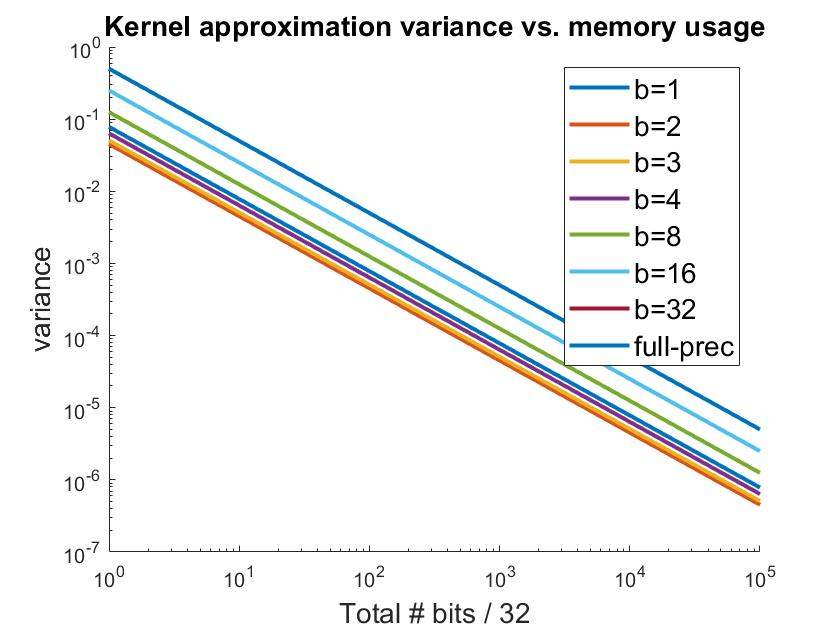
\includegraphics[width=0.6\textwidth]{lprff_variance_figure_numbits.jpg}
\end{center}
As you can see, lowering the precision helps reduce the variance by approximately a full order of magnitude ($10\times$ smaller variance) for a fixed number of bits, with $b=2$ giving the lowest variance, and $b=32$ variance matching the full-precision line (they are overlapping in the figure).  In the plot below, we show the kernel approximation variance as a function of the number of features.  As you can see, using $1$ bit per feature gives a noticeable jump in variance, but all other higher precision features perform comparably to the full-precision random features.
**OUTDATED**
\begin{center}
	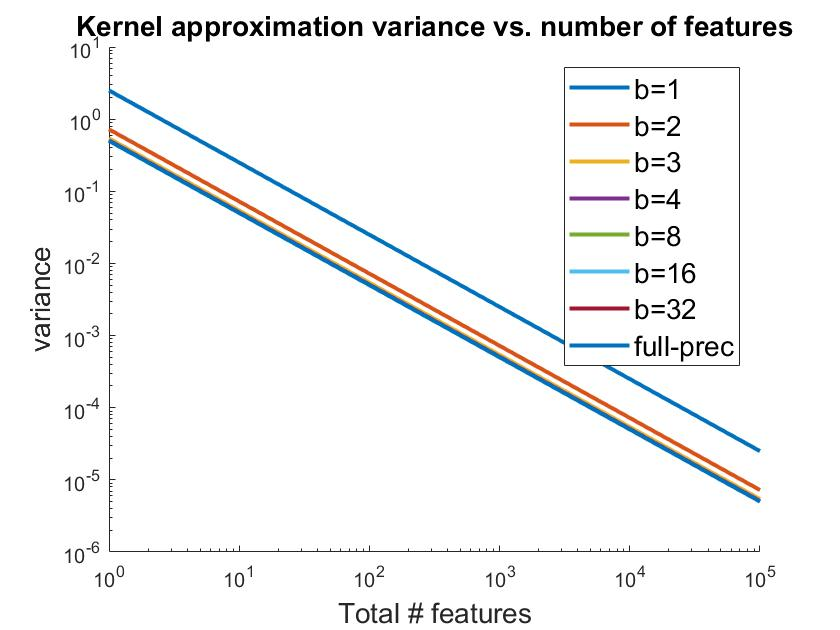
\includegraphics[width=0.6\textwidth]{lprff_variance_figure_numfeat.jpg}
\end{center}
% FIGURES
%figure; hold on;
%n = 1:100000;
%for b = [1,2,3,4,8,16,32]
%plot(n,(  (1/2) + 2/(2^(2*b)-2^(b+1)+1)  ) ./ n,'LineWidth',2)
%end
%plot(n,0.5./n,'LineWidth',2)
%lgd = legend('b=1','b=2','b=3','b=4','b=8','b=16','b=32','full-prec');
%lgd.FontSize = 14;
%xlabel('Total # features','FontSize',14)
%ylabel('variance','FontSize',14)
%title('Kernel approximation variance vs. number of features','FontSize',14)
%set(gca,'yscale','log')
%set(gca,'xscale','log')
%
%figure; hold on;
%n = 1:100000;
%for b = [1,2,3,4,8,16,32]
%plot(n,(  (1/2) + 2/(2^(2*b)-2^(b+1)+1)  ) ./ ((32/b) * n),'LineWidth',2)
%end
%plot(n,0.5./n,'LineWidth',2)
%lgd = legend('b=1','b=2','b=3','b=4','b=8','b=16','b=32','full-prec');
%lgd.FontSize = 14;
%xlabel('Total # bits / 32','FontSize',14)
%ylabel('variance','FontSize',14)
%title('Kernel approximation variance vs. memory usage','FontSize',14)
%set(gca,'yscale','log')
%set(gca,'xscale','log')
%



\item It is important to note that Propositions 2 and 3 hold as a function of the number of low-precision features, and \textit{match} the bounds for the \textit{same number} of high-precision features.\footnote{Some care is needed for Proposition 3, because the set of functions $\cF_p$ we are considering is different than the one in the original.  I believe I can show that for a properly defined set of quantization functions, our $\cF_p$ is a superset of the original, though I may need to update the constant $C$.}  This is pretty amazing!
\end{enumerate}

\subsection{Open Questions}
\begin{enumerate}
	\item Can we extend Claim 1 (Uniform convergence of Fourier features) from $[5]$ (Rahimi and Recht, 2007) to low-precision features $z(x)$, to prove that the probability that there exists $x,y\in\cX$ such that $|z(x)^Tz(y) -k(x,y)| \geq \eps$ is small?
	\item Can we perform training in such a way that the learned weights are also low-precision?  What guarantees can we get with a training algorithm of this form?
	\item How does the family of functions $\cF_p$ defined in Proposition 3 compare to the one in $[4]$ (Rahimi and Recht, 2008)?	
	%\item What can we say about the spectrum of the low-precision features relative to the full-precision features, and the exact kernel?  Results here would allow us to apply the ``fixed design'' linear regression analysis (from my other notes) here.
	\item Can we use low-precision for $x$,$w$, and $b$ in the features $z(x) = \sq\cos(w^Tx+b)$?  What can we prove about this?
\end{enumerate}

\section{Motivation}
Random Fourier features are an effective way of scaling kernel methods to large datasets.  Unfortunately, this method often requires a very large number of features in order to attain strong performance.  For example, in my work in speech recognition, increasing the number of features from 100k to 400k continued to give meaningful improvements.  At this scale, the amount of memory and computation time required to train models becomes a big bottleneck. For example, the size of a GPU's global memory can limit the number of random features which can be used, if one would like to train the model fully on a single GPU.  

Furthermore, in my work comparing random Fourier features and the \Nystrom method, I observed that using \textit{many} random Fourier features allows for approximating a larger portion of the kernel's spectrum, which appears to be important for attaining strong performance. This is in contrast to the \Nystrom method, which under a similar computational budget, computes fewer more expensive features; although these features approximate the kernel matrix very well, they are inherently limited in how many of the kernel's eigenvalues they can approximate.  The take-away here appears to be: many cheap features is better than fewer expensive features, even if those expensive features approximate the kernel matrix very well.

In light of the computational bottleneck which arises when training models with very many random features, as well as the observation that using a large number of features is important for downstream performance (even if they have higher variance when approximating the kernel), I propose using \textit{low-precision} as a way to further scale these random feature methods.
Some challenges involved in implementing and analyzing this idea are as follows:

\begin{enumerate}
	\item What are the trade-offs in deciding the number of bits of precision which should be used for the data, the random projection matrix, the random features, and the model parameters?  Can we effectively learn models on single-bit random features?
	\item If the model is stored in low-precision, what optimization algorithm should be used during training in order to make this possible?
	\item Will the final model be low-precision or high-precision?  Another way of asking this is: Is low-precision a trick to speed up the training of a full-precision model (as in HALP), or will the entire system be low-precision at both train and test time?
	\item How can we formalize the way the additional noise caused by quantization will affect the training of the model?  Can we use variance reduction techniques like SVRG to deal with this, like in HALP?
	\item Can we somehow use this additional randomness in the feature generation process in order to generate ``error bars'' in the estimates of the trained model (\eg, by evaluating the model on several random draws of the randomly quantized features for the same data point, in order to produce a distribution of predictions)?
\end{enumerate}

I will now discuss a few ideas related to two aspects of this project: (1) computing the random features, and (2) training a model with these features.

\section{Computing the low-precision random features}
Here, I will discuss different ways of computing $\tz(x)$, the quantized version of $z(x) = \sqrt{\frac{2}{m}} \cos(W^T x + b) \in \RR^m$, where $x\in \RR^d$, $W\in \RR^{d\times m}$, $b \in \RR^m$, and $\cos(\cdot)$ is the element-wise cosine non-linearity. Note that below I will ignore the factor of $\sqrt{\frac{2}{m}}$, as it can be stored separately as the ``scale'' parameter $\delta$ of the $b$-bit low-precision representation $(\delta,b)$.
\begin{itemize}
	\item Compute $\cos(W^Tx + b)$ using full precision (where $W$ can be a structured random matrix to save time/space), and then quantize the output.
	\item First, quantize $x$, $W$, and $b$, as $\tx$, $\tW$, $\tb$.  Then, compute $\tW^T \tx + \tb$, pass this 
	through the cosine function, and quantize the output.
	\item Use low-precision floating point operations (eg, 16-bit) for all of the operations.
\end{itemize}
One important thing to note is that quantizing $x$,$W$, and $b$ in such a way that $\expect{\tx,\tW,\tb}{\tW^T\tx + \tb} = W^Tx+b$ does \textit{not} mean that $\expect{\tx,\tW,\tb}{\cos(\tW^T\tx + \tb)} = \cos(W^Tx + b)$.  Thus, features generated in this way would not necessarily produce unbiased estimates of the kernel function, which satisfy $\expect{}{z(x)^Tz(y)} = k(x,y)$.
For this reason, I think the first option above is likely the best path forward.

In the case of 1-bit random features, we could quantize as follows: Let $z_i'(x) = \cos(w_i^T x + b_i)$ be the unnormalized $i^{th}$ feature of $z(x)$, and let $\tz_i'(x)$ be its quantized version, which we are discussing.  
In order for $\expect{}{\tz_i'(x)} = z_i'(x)$, we could set $\tz_i'(x) = +1$ with probability $\frac{1 + z_i'(x)}{2}$, and $\tz_i'(x) = -1$ with probability $\frac{1 - z_i'(x)}{2}$.  Here, we were using $\tz_i'(x) \in \{-1,+1\}$.
Note that one can simulate storing a vector $x \in \{-1,+1\}^d$ as a binary vector $\hat{x}\in \{0,1\}^d$ by noticing that 
$\dotp{x,y}= 2 \dotp{\hat{x},\hat{y}} - d$.

\section{Training a model using low-precision random features}
In this section, we address the question of how to train a model using low-precision random features as input.  Essentially, this comes down to training a linear model on top of random features $\tz$ such that $\expect{}{\tz} = z$.  One potentially
great option is to use ``LM-HALP'', the version of HALP designed for learning linear models, presented as Algorithm 4 in the
recent submission.  One potential down-side to this approach is that it would mean that the learned model would be
full-precision, which may or may not be desirable (for example, computing the full-precision gradient over the entire dataset
could be prohibitively expensive, and perhaps even impossible in the case where the full-precision model doesn't fit in
memory).  Note that any of the options below which use low-precision for both train/test would be inherently limited in terms of
how close to the global optimum they could get, as discussed in the HALP paper.  Perhaps, however, the error introduced by this
quantization could be more than made-up for by the ability to learn a model in a higher-dimensional, more expressive, feature
space.  We present some alternative options to LM-HALP below:
\begin{itemize}
	\item \textbf{Perceptron updates}: We could use the perceptron algorithm for model updates, 
	which would ensure that all operations could be done in integer arithmetic.
	\item\textbf{ Quantized SGD updates (``LP-SGD'')}: Consider the full-precision SGD update of
	the form $w_{t+1} = w_t + g_t z_t$, where $z_t = z(x_t) \in \RR^m$ is the random
	feature representation corresponding to the randomly chosen training point $x_t$ at
	time $t$.  We could replace this update by updates of the form 
	$w_{t+1} = w_t + \tg_t \tz_t$, where $\expect{}{\tg_t} = g_t$, and $\tg_t$ is stored in
	low-precision format.  For example, in the case of logistic regression, 
	$g_t = \eta \big(y_t - p_t\big)$, where $y_t\in\{0,1\}$ is the label for $x_t$, $\eta \in \RR$ is the learning
	rate, and $p_t = p(Y_t=1|z_t,w_t) = (1+\exp(-w_t^Tz_t))^{-1}$.  So in the case where $y_t = 1$,
	$\tg_t$ could be equal to $1$ with probably $1-p_t$, and 0 otherwise; and in the case
	where $y_t = 0$, $\tg_t$ could be equal to $-1$ with probability $p_t$, and 0
	otherwise.  Here, I am assuming that $\eta$ is stored in the scale factor $\delta$
	of the low-precision format $(\delta,b)$ for $\tg_t$.	
	If $\tg_t$ is in $(\delta,b)$ low-precision format, and $\tz_t$ is in
	$(\delta',b')$ format, then $w_t$ would be in $(\delta\delta',b+b')$ format.
	Note also that computing $p_t$ requires using the $\exp(\cdot)$
	and $(\cdot)^{-1}$ operations, which would probably need to be done as floating point
	operations.
	\item \textbf{LP-SVRG}: We could directly use LP-SVRG.
	\item \textbf{Update dual variables instead of primal}: In terms of the dual variables $\alpha_i$, the
	model becomes $f(x) = \sum_{i=1}^n \alpha_i z(x_i)^T z(x)$. Letting 
	$Z\in \RR^{n\times m}$ be the matrix whose $i^{th}$ row is $z(x_i)$, this can be
	rewritten as $\alpha^T (Z z(x))$.  If the random features are binary, $Zz(x)$ 
	can be implemented very efficiently, and its output is an integer vector (note that for huge $Z$,
	this operation can be distributed across a cluster of machines).
	If $\alpha$ is stored in low-precision format (as it would be if updates of the form described above
	for perceptron or LP-SGD are used), this dot-product could be performed using low-precision
	integer arithmetic, which can also be implemented fast.  As far as updating the values of
	the dual parameters $\alpha_i$ during training, we can simply simulate the primal updates of the form 
	$w_{t+1} = w_t + \tg_t z_t$ by using $\alpha_t = \alpha_t + \tg_t$, where here I am using 
	$\alpha_t$ to denote the dual parameter corresponding to the random point $x_t$ chosen at time $t$.
	\item \textbf{Distributed optimization}: We could also consider large-scale distribution optimization algorithms (\eg, $[1,2]$) in order to speed up training.
\end{itemize}

\section{Kernel Approximation Variance Analysis for Low-Precision RFF}
\noindent\textbf{Definitions}: For $z \in [a,c]$, let $X_z^{a,c}$ be the random variable which with probability $\frac{z-a}{c-a}$ equals $c-z$, and with probability $\frac{c-z}{c-a}$ equals $a-z$. Furthermore, let $Q^{a,c}(z) = z + X_z^{a,c} \in \{a,c\}$ be the ``quantized'' version of $z$, corresponding to randomized rounding to $a$ or $c$. \\

\noindent\textbf{Lemma 1}: Using the definitions above, it follows that $\expect{}{X_z^{a,c}} = 0$, $\var{}{X_z^{a,c}} = (z-a)(c-z)$, $\expect{}{Q^{a,c}(z)} = z$, and $\var{}{Q^{a,c}(z)} = (z-a)(c-z) \leq \frac{(c-a)^2}{4}$.\\

\noindent\textbf{Proposition 1}: For $x,y\in\cX$, assume we have random variables $Z_x,Z_y$ satisfying $\expect{}{Z_xZ_y} = k(x,y)$, and $\var{}{Z_x} = \sigma^2$, and that $k(x,x) = k(y,y) = 1$.\footnote{For example, one specific instance of the random variables $Z_x,Z_y$ is given by random Fourier features, where $z_x = \sq\cos(w^Tx+b),z_y = \sq\cos(w^Ty+b)$, $z_x,z_y\in[-\sq,\sq]$, for random $w,b$.}  For any unbiased random quantization function $Q$ with bounded variance $\var{}{Q(z)} \leq \tsigma^2$ for any $z$, it follows that $\expect{}{Q(Z_x)Q(Z_y)} = k(x,y)$, and that $\var{}{Q(Z_x)Q(Z_y)} \leq 2\tsigma^2 + \tsigma^4 + \sigma^2$.\\

\noindent\textit{proof}: Let $Q(Z_x) = Z_x + \eps_x$, and $Q(Z_y) = Z_y + \eps_y$, where $\expect{}{\eps_x} =\expect{}{\eps_y} = 0$ and $\expect{}{\eps_x^2} \leq \tsigma^2$, $\expect{}{\eps_y^2} \leq \tsigma^2$.

\begin{eqnarray*}
\expect{}{Q(Z_x)Q(Z_y)} &=& \expect{}{(Z_x + \eps_x)(Z_y + \eps_y)} \\
&=& \expect{}{Z_xZ_y + Z_y \eps_x + Z_x \eps_y + \eps_x \eps_y} \\
&=& \expect{}{Z_xZ_y} \\
&=& k(x,y).
\end{eqnarray*}
\begin{eqnarray*}
\var{}{Q(Z_x)Q(Z_y)} &=&  \expect{}{\Big(Q(Z_x)Q(Z_y) - k(x,y)\Big)^2} \\
&=& \expect{}{\Big((Z_x + \eps_x)(Z_y + \eps_y) - k(x,y)\Big)^2} \\
&=& \expect{}{\Big(Z_y \eps_x + Z_x\eps_y + \eps_x \eps_y +  Z_xZ_y - k(x,y)\Big)^2} \\
&=& \expect{}{\Big(Z_y \eps_x + Z_x\eps_y + \eps_x \eps_y\Big)^2} +  \expect{}{\Big(Z_xZ_y - k(x,y)\Big)^2} \\
&=& \expect{}{Z_y^2 \eps_x^2 + Z_x^2\eps_y^2 + \eps_x^2 \eps_y^2} +  \sigma^2 \\
&\leq& k(y,y) \tsigma^2 + k(x,x) \tsigma^2 + \tsigma^4 +  \sigma^2 \\
&\leq& 2\tsigma^2 + \tsigma^4 +  \sigma^2. 
\end{eqnarray*}

\noindent\textbf{Proposition 2}: Let $Q$ be any unbiased quantization function with bounded variance ($\expect{}{Q(z)} = z$, $\var{}{Q(z)} \leq \tsigma^2$ for any $z$).  Let $S=Z_x Z_y$, $T = Q(Z_x)Q(Z_y)$, and $(S_1,\ldots,S_n)$, $(T_1,\ldots,T_n)$ be a random sequence of i.i.d. draws from $S$ and $T$ respectively.  Define $\bar{S}_n = \frac{1}{n}\sum_{i=1}^n S_i$, and $\bar{T}_n =  \frac{1}{n}\sum_{i=1}^n T_i$, to be the empirical mean of these draws.  It follows that $\expect{}{\bS_n} = \expect{}{\bT_n} = k(x,y)$, and that
$\var{}{\bS_n} = \frac{\sigma^2}{n}$, and $\var{}{\bT_n} \leq \frac{2\tsigma^2 + \tsigma^4 +  \sigma^2}{n}$.\\

Now, let's analyze the variance of using $\bS_n$ to approximate $k(x,y)$, relative to $\bT_{n*(32/b)}$.  This corresponds to comparing the variance of using $n$ ``full precision''  features (which we will assume are 32-bit), relative to using $n*(32/b)$ $b$-bit low-precision features. Note that both of these feature representations use the same total number of bits.  We will in this case assume we are using random Fourier features, and thus that
$z_x,z_y \in [-\sq,\sq]$.  We will upper bound $\sigma^2$ in this context by $1$, given the results in $[3]$ for the RBF kernel.  Furthermore, it is important to note that the quantization noise $\tsigma^2$ is very much tied to the number of bits used to quantize the features $z_x$.  We will thus use $\tsigma_b^2$ to denote the variance introduced by quantizing into $b$-bits.  In this case, we divide the interval $[-\sq,\sq]$ into $2^b-1$ sub-intervals of equal size, and quantization is performed within each of these intervals; each interval is of size $r = \frac{2\sq}{2^b-1}$. 
Thus, from Lemma 1 (see footnote) the quantization error $\tsigma_b^2 \leq r^2/4 = \frac{2}{(2^b-1)^2}$.  This allows us to perform the comparison discussed above:

\begin{eqnarray*}
	\var{}{\bS_n} &=& \frac{\sigma^2}{n} \\
	&\leq& \frac{1}{n}. \\
	\var{}{\bT_{n*(32/b)}} &\leq& \frac{2\tsigma_b^2 + \tsigma_b^4 +  \sigma^2}{n*(32/b)} \\
	&\leq& \frac{2\frac{2}{(2^b-1)^2}  + \big(\frac{2}{(2^b-1)^2}\big)^2+ 1}{n*(32/b)}\\
	&\leq& \frac{\frac{4}{(2^b-1)^2} + \frac{4}{(2^b-1)^4} +  1}{n*(32/b)}\\
\end{eqnarray*}

We now plot these two upper bounds on a log-log plot, for various values of $b$ and $n$.\\
**OUTDATED**
\begin{center}
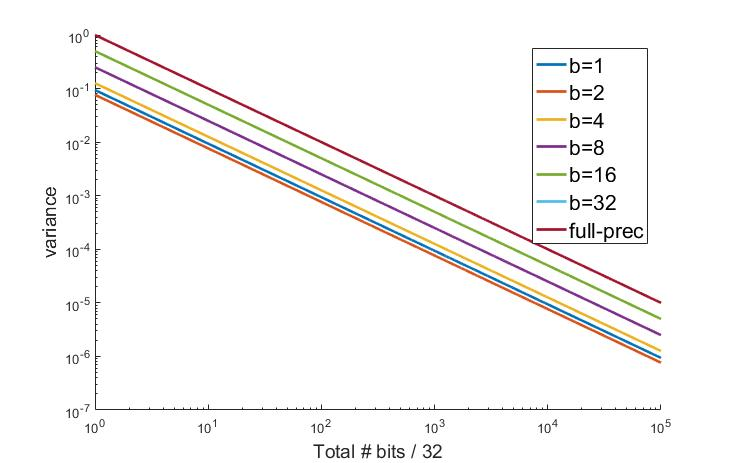
\includegraphics[width=0.6\textwidth]{lprff_variance_figure.jpg}
\end{center}
As you can see, lowering the precision helps reduce the variance by approximately a full order of magnitude ($10\times$ smaller variance), with $b=2$ giving the lowest variance, and $b=32$ variance matching the full-precision line (they are overlapping in the figure).

I will now discuss a concentration bound for these low-precision random features:\\
\textbf{Proposition 2}: For a fixed $x,y\in\cX$, let $S$ be any random variable with the property that $\expect{}{S} = k(x,y)$, and $S \in [-2,2]$.  Let $(S_1,\ldots,S_n)$, be a random sequence of i.i.d. draws from $S$, and let $\bS_n = \frac{1}{n}\sum_{i=1}^n S_i$ be the empirical mean of this sequence.  Then, it follows directly from Hoeffding's inequality that $\Prob{\big[|\bS_n - k(x,y)| \geq \epsilon\big]} \leq 2\exp(-n\eps^2/8)$.

\textbf{Open Question}: Can Claim 1 from Rahimi and Recht (2007) be adapted to this low-precision setting?  The most obvious obstacle here is that the randomness depends on the data; in other words, each $x \in \RR$ has a unique quantization noise distribution.  In other words, with the current definition, there is no way to draw all the random feature parameters upfront, in such a way that given these parameters, the feature functions are deterministic.  Can we somehow switch the quantization scheme for it to be deterministic?  For example, splitting the interval $[-\sq,\sq]$ into $r$ sub-intervals---then, for interval

\section{Variance introduced at test time}
Assume we have learned a model $w$ over an RFF representation (low precision or full precision, doesn't matter).  We now consider the expected value for $(w^T z(x) - y)^2$, relative to $(w^T (z(x) + \eps_x) -y)^2$, where $z(x)$ denotes the full precision RFF representation for $x$, and $z(x) + \eps_x$ represents the randomly quantized representation.
\begin{eqnarray*}
	\expect{}{(w^T (z(x) + \eps_x) -y)^2} &=& \expect{}{(w^T z(x) + w^T \eps_x -y)^2} \\
	&=& \expect{}{(w^T z(x) - y)^2)} + \expect{}{(w^T \eps_x)^2} \\
	&=& \expect{}{(w^T z(x) - y)^2)} + \expect{}{\Big(\sum_i w_i \eps_{x,i}\Big)^2} \\
	&=& \expect{}{(w^T z(x) - y)^2)} + \sum_i w_i^2 \expect{}{\eps_{x,i}^2} \\
	&=& \expect{}{(w^T z(x) - y)^2)} + \|w\|^2\expect{}{\eps_{x,1}^2} \\
	&\leq& \expect{}{(w^T z(x) - y)^2)} + \|w\|^2\cdot\frac{1}{4}\bigg(\frac{2\sqrt{2/d}}{2^b-1}\bigg)^2\\
	&=& \expect{}{(w^T z(x) - y)^2)} + \|w\|^2\cdot\frac{2}{d(2^b-1)^2}.
\end{eqnarray*}

In other words, our expected error on a test point $(x,y)$, if we use quantized features at test time, is in expectation $\|w\|^2\cdot\frac{2}{d(2^b-1)^2}$ larger than the expected error if we used the full precision features at test time.  This suggests that it could be desirable, in certain contexts, to train using low precision (to speed up training), but use full precision features at test time.

\section{``Deterministic'' Quantization Functions}
In Proposition 3, we defined a set of deterministic quantization functions
$\{Q_{\theta}:\RR\rightarrow\RR \;|\; \theta\in\Theta \}$, parameterized by some parameter $\theta\in\Theta$.
We now discuss how to construct these.  The idea is simple: For every quantization interval $[a,c]$, we choose a threshold value $t \in [a,c]$ uniformly at random.  Then if a certain unquantized feature $z$ falls in this interval, we will set $Q_t(z)= a$ if $z \leq t$, and $Q_t(z) = c$ if $z > t$.  It is easy to show that $\expect{t}{Q_t(z)} = z$:
\begin{eqnarray*}
	\expect{t}{Q_t(z)} &=& a \cdot \Prob[z \leq t] + c \cdot \Prob[z > t]  \\
	&=& a \cdot \frac{c-z}{c-a} + c\cdot \frac{z-a}{c-a} \\
	&=& \frac{ac - az + cz - ac}{c-a} \\
	&=& z.
\end{eqnarray*}
Thus, if for every quantization interval we draw a random threshold $t_i$ as described, and concatenate these thresholds as $\theta = (t_1,\ldots,t_{2^b-1})$, we have successfully constructed a set of unbiased and deterministic quantization functions, as desired.


%We now discuss how to apply the result from Theorem 1 of Rahimi and Recht's 2008 paper to this low-precision setting [4].  That theorem assumes that there is a set of (deterministic) basis functions $\phi: \cX \times \Omega \rightarrow \RR$.  It then argues that if $\{w_1,\ldots,w_K\}$ are drawn independently from some distribution $p$ on $\Omega$, then the generalization performance of the model trained on the features $\phi(\;\cdot\;;w_i)$ is close to the best possible generalization performance of any model in the set $\cF_p = \{f(x) = \int_\Omega \alpha(w)\phi(x;w)dw | |\alpha(x)| \leq Cp(w)\}$.  Unfortunately, our randomly quantized features currently do not fit nicely into this framework, because the basis functions themselves are random, even for a fixed $x$ and $w$.  The purpose of the section below is to construct a parametrized set of basis functions $\phi(x;w,b,\theta)$ which quantize $\cos(w^Tx+b)$ in a deterministic way, given the parameters $\theta$.  

\section{Why low-precision spectra are elevated}
\label{sec:elevate_spectrum}
In this section, we explain our empirical observation that the spectra of our kernel approximation matrices are much higher than the actual spectrum of the exact kernel matrix, in the case where we use 1, 2, or 4 bits to quantize our features.  If we consider the $n$ by $d$ RFF matrix $Z$, whose $i^{th}$ row is $z(x_i)$, and let $C$ denote the zero mean random quantization noise which is added to $Z$, it is easy to see that the kernel approximation matrix $(Z+C)(Z+C)^T$ has an elevated spetrum $\tlambda$, because:
\begin{eqnarray*} 
\expect{}{\sum_i \tlambda_i} &=& \expect{}{trace[(Z+C)(Z+C)^T]} \\
&=& \expect{}{trace[ZZ^T] + trace[ZC^T] + trace[CZ^T] + trace[CC^T]}\\
&=& trace[ZZ^T] + \expect{}{trace[CC^T]} \\
&>& trace[ZZ^T] \\
&=& \expect{}{\sum_i \lambda_i}
\end{eqnarray*}
Notice that the spectrum $\tlambda$ of $(Z+C)(Z+C)^T$ relates to the spectrum $\tsigma$ of $(Z+C)$ via $\tlambda_i = \tsigma_i^2$.  Thus, letting $\sigma$ denote the spectrum of $Z$, we have shown that
$\expect{}{\sum_i \tsigma_i^2} > \sum_i \sigma_i^2$.  In other words, adding zero mean noise of any kind to a matrix elevates the $\ell_2$ norm of its spectrum.  This is intuitive because the noise will always increase the total weight on the diagonal of $ZZ^T$.
More interestingly, however, we can also show that if we take two random draws $C$ and $D$ of the quantization noise, the spectrum of $(Z+C)(Z+D)^T$ is also elevated relative to $ZZ^T$, even though the expected value of the entries of the diagonal of this matrix are \textit{equal} to the entries of the $ZZ^T$ diagonal.  This is because we can write $(Z+C)(Z+D)^T = ZZ^T + CZ^T + ZD^T + CD^T = ZZ^T + N$, where $N = CZ^T + ZD^T + CD^T$ is zero mean noise.  Thus, just like the spectrum of $Z+C$ was higher than that of $Z$ because we added zero mean noise $C$ to it, the spectrum of $(Z+C)(Z+D)^T$ will be higher than that of $ZZ^T$ because we are adding zero mean noise $N$ to it.  We show this in more detail below:

\begin{eqnarray*}
	A &=& ZZ^T \\
	&=& USU^T \\ %= \sum_i \lambda_i u_i u_i^T \\
	trace(A^T A) &=& trace( USU^T U S U^T)\\
	&=& trace( US^2 U^T) \\
	&=& \sum_i{\lambda_i^2}\\
	\tA &=& (Z+C)(Z+D)^T \\
	%	    &=& VTV^T \\
	\tA^T\tA &=& (Z+D)(Z+C)^T(Z+C)(Z+D)^T \\
	&=& ZZ^TZZ^T + ZC^TCZ^T + DZ^TZD^T + DC^TCD^T + \text{zero-mean}\\ 
	&=& A^TA + ZC^TCZ^T + DZ^TZD^T + DC^TCD^T + \text{zero-mean}\\ 
\end{eqnarray*}
\begin{eqnarray*}
	trace(\tA^T\tA) &=& trace(A^TA) + trace(ZC^TCZ^T) + trace(DZ^TZD^T) + trace(DC^TCD^T) + trace(\text{zero-mean})\\ 
	&=& \sum_i \tilde{\lambda_i}^2\\
	\expect{}{\sum_i \tilde{\lambda_i}^2} &=& \expect{}{trace(\tA^T\tA)} \\
	&=& trace(A^TA) + \expect{}{trace(ZC^TCZ^T) + trace(DZ^TZD^T) + trace(DC^TCD^T)} + \expect{}{trace(\text{zero-mean})}\\
	&=& trace(A^TA) + \expect{}{trace(ZC^TCZ^T) + trace(DZ^TZD^T) + trace(DC^TCD^T)}\\	
	&\geq& trace(A^TA) \\
	&=&  \sum_i{\lambda_i^2}. \\
	%\expect{}{z^T \tA^T\tA z} &=& z^TA^TAz + \expect{}{z^T(ZC^TCZ^T + DZ^TZD^T + DC^TCD^T)z} + %\expect{}{z^T\text{zero-mean}z}\\ 
	%&\geq& z^TA^TAz 
\end{eqnarray*}
%So taking $z = u_i$, we get $\|\tA u_i\|^2 \geq \|Au_i\|^2 = \lambda_i^2$.
%Can we show $\tA-A$ is PSD?

Now, we ask the following question: How large is the expected gap between $\expect{}{\sum_i \tilde{\lambda_i}^2}$ and $\sum_i{\lambda_i^2}$? To answer this, we consider the magnitude of 
$\expect{}{trace(ZC^TCZ^T) + trace(DZ^TZD^T) + trace(DC^TCD^T)}$, relative to the magnitude of
$\expect{}{trace[ZZ^TZZ^T]}$.  We begin by simply getting a simpler expression for $trace[AB^TBA^T]$ for
arbitrary matrices $A$ and $B$.\\

\noindent\textbf{Lemma}: $trace[AB^TBA^T] = \sum_{i,j=1}^n \sum_{k,\hk=1}^d a_{jk}a_{j\hk}b_{ik}b_{i\hk}$.\\

\noindent \textbf{Proposition}:  $\expect{}{trace[ZZ^TZZ^T]} = n + \frac{n^2-n}{d}$, while 
$\expect{}{trace(ZC^TCZ^T) + trace(DZ^TZD^T) + trace(DC^TCD^T)} = \frac{4n^2}{d(2^b-1)^2} + \frac{4n^2}{d(2^b-1)^4} = \frac{4n^2}{d}\Big(\frac{1}{(2^b-1)^2} + \frac{1}{(2^b-1)^4}\Big)$. \\

\noindent \textit{Proof}:  We will use the above Lemma to compute expected values for $trace[ZZ^TZZ^T]$, $trace(ZC^TCZ^T)$, $trace(DZ^TZD^T)$, and $trace(DC^TCD^T)$.  This will directly prove the proposition.

\begin{itemize}
\item Case 1: $A=B=Z$.
\begin{eqnarray*}
\expect{}{trace[ZZ^TZZ^T]} &=& \sum_{i,j=1}^n \sum_{k,\hk=1}^d \expect{}{z_{jk}z_{j\hk}z_{ik}z_{i\hk}}\\
&=& \sum_{i=1}^n \sum_{k,\hk=1}^d \expect{}{z_{ik}^2}\expect{}{z_{i\hk}^2} + \sum_{i\neq j} \sum_{k=1}^d \expect{}{z_{jk}^2}\expect{}{z_{ik}^2}\\
&=& \sum_{i=1}^n \sum_{k,\hk=1}^d \frac{1}{d^2} + \sum_{i\neq j} \sum_{k=1}^d \frac{1}{d^2}\\
&=& nd^2\frac{1}{d^2} + (n^2-n)d\frac{1}{d^2}\\
&=& n + \frac{n^2-n}{d}.
\end{eqnarray*}
Above, we used the fact that $\expect{}{z_{ik}^2} = \expect{w_k,b_k}{\frac{2}{d}\cos(w_k^T x_i + b_k)^2} = \frac{k(x_i,x_i)}{d} = \frac{1}{d}$.
\item Case 2: $A=Z$, $B=C$ (or $A=D$ and $B=Z$).
\begin{eqnarray*}
\expect{}{trace[ZC^TCZ^T]} &=& \sum_{i,j=1}^n \sum_{k,\hk=1}^d \expect{}{z_{jk}z_{j\hk}c_{ik}c_{i\hk}}\\	
&=& \sum_{i,j=1}^n \sum_{k=1}^d \expect{}{z_{jk}^2}\expect{}{c_{ik}^2}\\	
&\leq& \sum_{i,j=1}^n \sum_{k=1}^d \frac{1}{d}\cdot \frac{1}{4}\bigg(\frac{2\sqrt{2/d}}{2^b-1}\bigg)^2\\	
&=& n^2d \cdot \frac{1}{d}\cdot \frac{1}{4}\cdot \frac{8}{d(2^b-1)^2}\\	
&=& \frac{2n^2}{d(2^b-1)^2} \\
&=& O\Big(\frac{n^2}{d\cdot 2^{2b}}\Big).
%&\approx& \frac{2n^2}{d2^{2b}} \\
%&=& \frac{n^2}{d}\Big(2^{-2b+1}\Big) \\
\end{eqnarray*}
Above, we use the fact that $\expect{}{c_{ik}^2} \leq \frac{1}{4}\bigg(\frac{2\sqrt{2/d}}{2^b-1}\bigg)^2 = \frac{2}{d(2^b-1)^2}$, and that $\expect{}{z_{ik}^2} = \frac{1}{d}$.  Note that this bound also holds when $A=D$ and $B=Z$.
\item Case 3: $A=C$, $B=D$.
\begin{eqnarray*}
\expect{}{trace[CD^TDC^T]} &=& \sum_{i,j=1}^n \sum_{k,\hk=1}^d \expect{}{c_{jk}c_{j\hk}d_{ik}d_{i\hk}}\\
&=& \sum_{i,j=1}^n \sum_{k=1}^d \expect{}{c_{jk}^2}\expect{}{d_{ik}^2}\\
&=& \sum_{i,j=1}^n \sum_{k=1}^d \bigg(\frac{2}{d(2^b-1)^2}\bigg)^2\\
&=& n^2d \cdot\frac{4}{d^2(2^b-1)^4}\\
&=& \frac{4n^2}{d(2^b-1)^4}\\
&=& O\Big(\frac{n^2}{d \cdot 2^{4b}}\Big).
\end{eqnarray*}
\end{itemize}
This concludes the proof.
In this section, we compare the performance of LP-RFFs with full-precision RFFs (FP-RFFs), circulant FP-RFFs, and the \Nystrom method, on the TIMIT, YearPred, CovType, and Census datasets, showing that we can attain compression ratios of at least 2.4x relative to these methods, without hurting generalization performance. We then perform a more careful analysis of these results on the Census dataset and a sub-sampled version of the CovType dataset, where we plot the generalization performance of these approximation methods relative to their relative spectral distances. We observe on both datasets that the relative spectral distance appears much more predictive of generalization performance than more standard metrics like the Frobenius and spectral norms of $K-\tK$.  We note that in our experiments, in order to avoid the risk of numerical precision issues (kernel ridge regression requires matrix inversion), we do all our full-precision experiments in 64 bits.  Nonetheless, we calculate the memory utilization of these experiments as if we used 32 bits, to avoid inflating the relative gains of our method over the full precision approaches.

For all our experiments, we use the Gaussian kernel with the kernel width value recommended by~\citet{may2017}, and compute the memory utilization as described in Section~\ref{subsec:memory_utils}. To evaluate the performance of these kernel models, we measure the classification error for classification tasks, and the mean squared error (MSE) for regression tasks ($\frac{1}{n}\sum_{i=1}^n (f_{\tK}(x_i) - y_i)^2$), on the heldout set. We include more details about our datasets, experimental protocols, and hyperparameter choices in Appendix~\ref{sec:exp_details}.

\subsection{Empirical evaluation of LP-RFFs}
We compare the generalization performance of LP-RFFs to FP-RFFs, circulant FP-RFFs, and \Nystrom features, across four datasets, for various memory budgets.  We sweep the following hyperparameters: For LP-RFFs, we choose the precision $b \in \{1,2,4,8,16\}$. For \NystromNS, we use $m \in \{1250, 2500, 5000, 10000, 20000\}$.  For the RFF-based methods, we use $m\in \{1250, 2500, 5000, 10000, 20000, 50000, 100000, 200000, 400000\}$. We choose these limits differently because $\num[group-separator={,}]{20000}$ \Nystrom features have roughly the same memory footprint as $\num[group-separator={,}]{400000}$ FP-RFFs. For all experiments, we use a mini-batch size of $250$. We avoid the prohibitively large computational expense of performing a grid search to tune the initial learning rate, the regularizer, the learning rate decay, and the number of training epochs, by using the heldout set in order to determine learning rate decay \citep{morgan1990generalization,sainath2013b,sainath2013low}. The scheme works as follows: at the end of each epoch, we decay the learning rate in half if the heldout performance is less than $1\%$ better relative to the previous best model, using MSE for regression and cross entropy for classification. Furthermore, if the model performs \textit{worse} than the previous best, we revert the model. The training terminates after the learning rate has been decayed 10 times. Early stopping can be seen as a form of regularization \citep{zhang2005boosting,wei2017early}.  We use a single initial learning rate per dataset across all experiments, which we tune via grid search using $20\text{k}$ \Nystrom features. We choose to use \Nystrom features to tune the initial learning rate in order to avoid biasing the results in favor of RFF-based approaches. 

In Figure \ref{fig:generalization_col}, we plot the generalization performance for all these experiments, as a function of the amount of memory used, as well as the number of features $m$. We show across all four datasets that LP-RFFs show systematically better generalization performance than the full precision baselines under various memory budgets. Importantly, we see that the \Nystrom method has observably better generalization performance than LP-RFF and FP-RFF-based baselines under the same number of features. However, when we instead consider performance as a function of memory utilization, the opposite it true, with the RFF-based methods demonstrating superior generalization performance. This observation further validates the practical importance of comparing kernel approximation methods under memory budgets.

In Table~\ref{tab:mem_saving} we present the compression ratios we achieve with LP-RFFs, relative to the baselines, while still attaining generalization performance within $10^{-4}$ of the full-precision baseline.  We measure this as follows: For each baseline (FP-RFFs, circulant FP-RFFs, \Nystrom), we find the best performing (as well as median) model. We then find the smallest LP-RFF model, as well as the smallest baseline model, which attains within $10^{-4}$ relative performance to the best performing baseline.  We report the ratio of the memory used by these two models (baseline/LP-RFF), that are both within $10^{-4}$ of the best baseline. We compute this ratio across three independent runs using different random seeds, and report the average.  We can see that LP-RFFs demonstrate significant memory saving over FP-RFFs and circulant FP-RFFs, showing 2.9x-10.3x and 2.4x-15.6x compression ratios respectively. On the TIMIT dataset, there are 147 classes, and thus the full-precision learned parameters occupy a large portion of the total memory across all methods. Nonetheless, even though these LP-RFF experiments only quantize the feature mini-batches, they still attain 5.1x and 2.4x compression ratios relative to FP-RFF and circulant FP-RFF.

\begin{figure}
	\centering
	\begin{small}
	\begin{tabular}{@{\hskip -0.05in}c@{\hskip -0.1in}c@{\hskip -0.1in}c@{\hskip -0.1in}c@{\hskip -0.05in}}
%		\subfigure[YearPred MSE vs. Mem.]{\label{fig:year_pred_mem} 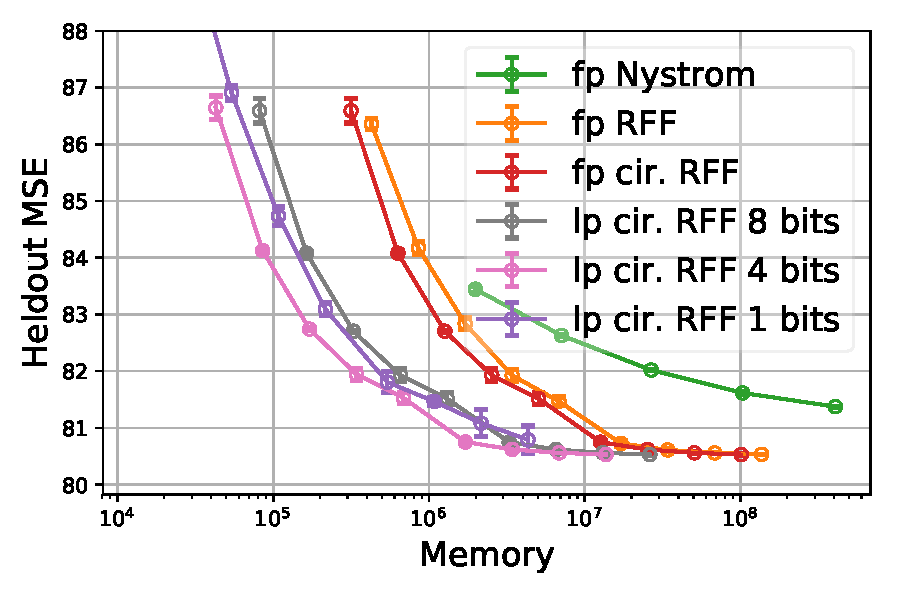
\includegraphics[width=0.27\linewidth]{figures/yearpred_MSE_vs_n_memory.pdf} } \hfill
%		\subfigure[TIMIT Err. vs. Mem.]{\label{fig:year_pred_mem} 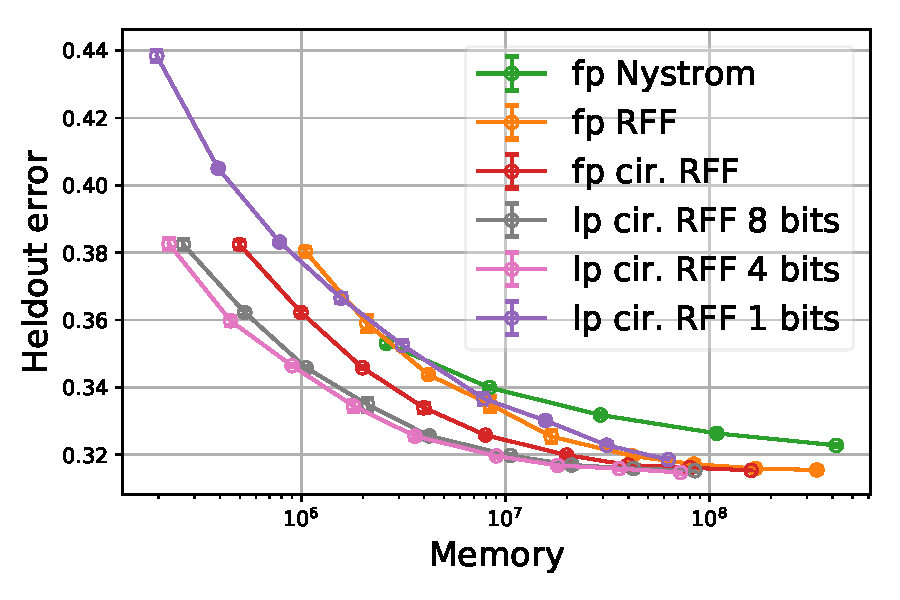
\includegraphics[width=0.27\linewidth]{figures/timit_error_vs_n_memory.pdf} } \hfill
%		\subfigure[YearPred MSE vs. Feat.]{\label{fig:year_pred_feat}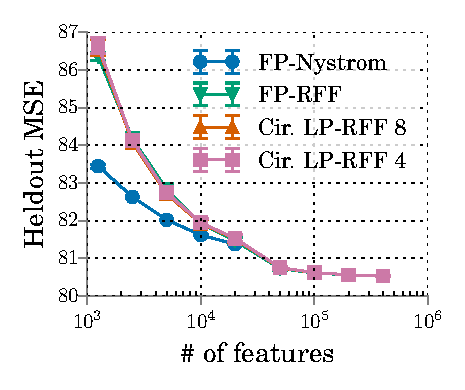
\includegraphics[width=0.27\linewidth]{figures/yearpred_MSE_vs_n_feat.pdf} } \hfill
%		\subfigure[TIMIT Err vs. Feat.]{\label{fig:year_pred_feat}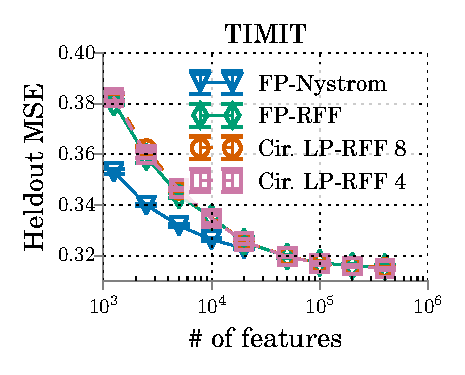
\includegraphics[width=0.27\linewidth]{figures/timit_error_vs_n_feat.pdf} } \hfill
		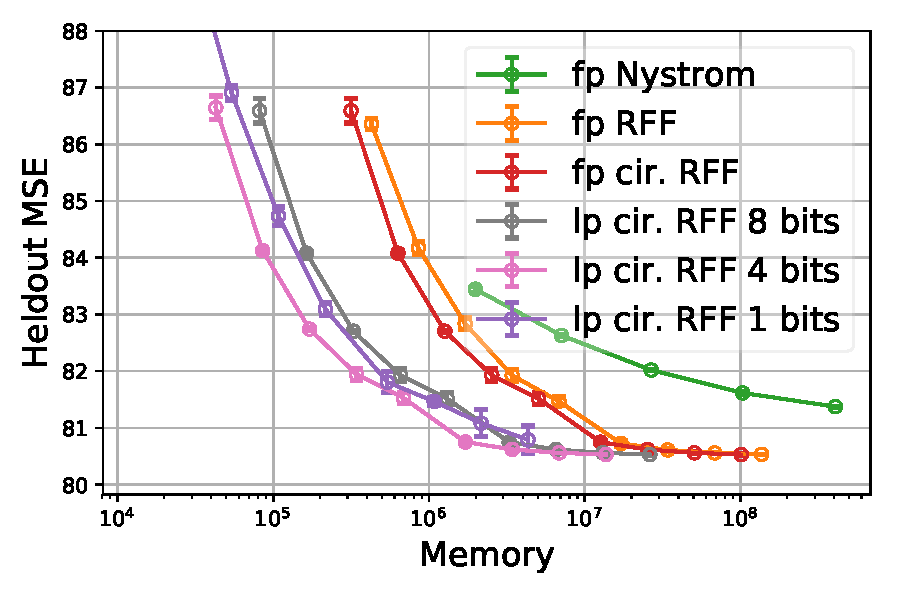
\includegraphics[width=0.27\linewidth]{figures/yearpred_MSE_vs_n_memory.pdf} &
		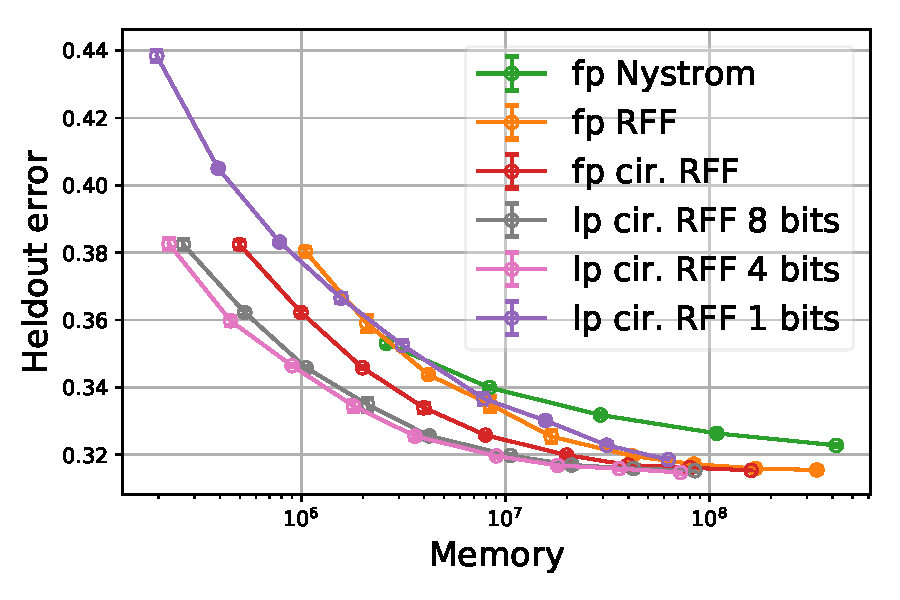
\includegraphics[width=0.27\linewidth]{figures/timit_error_vs_n_memory.pdf} &
		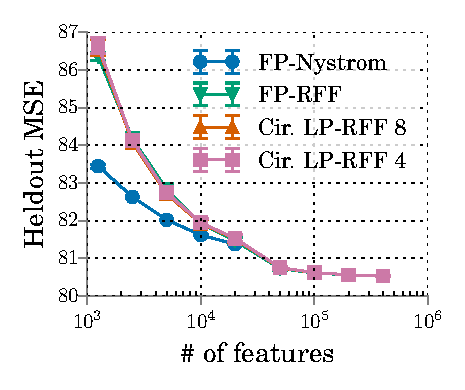
\includegraphics[width=0.27\linewidth]{figures/yearpred_MSE_vs_n_feat.pdf} &
		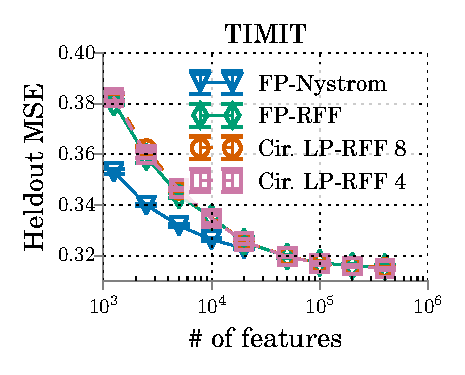
\includegraphics[width=0.27\linewidth]{figures/timit_error_vs_n_feat.pdf} \\
		(a) YearPred MSE vs. Mem. & (b) TIMIT Err. vs. Mem. & (c) YearPred MSE vs. Feat. & (d) TIMIT Err vs. Feat.\\
%		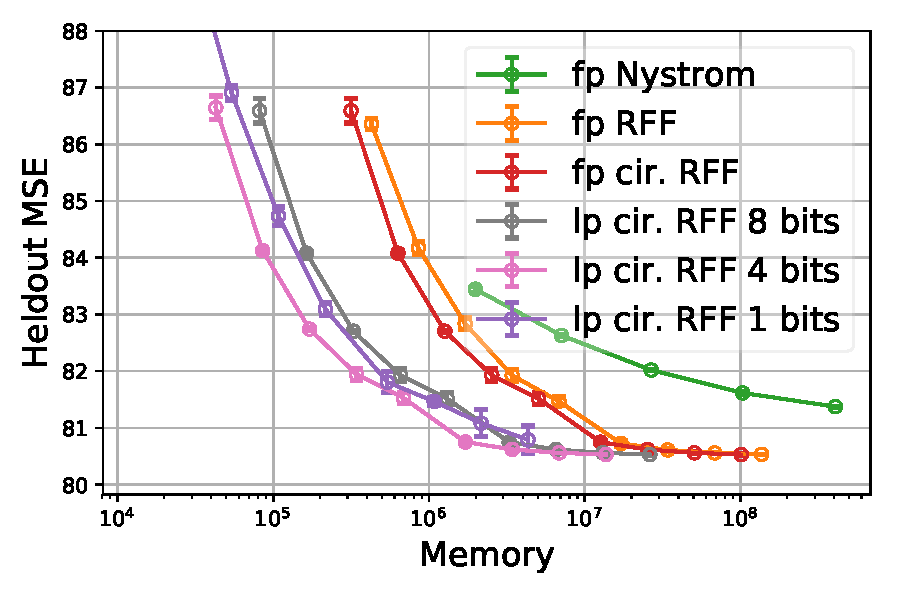
\includegraphics[width=0.3\linewidth]{figures/yearpred_MSE_vs_n_memory.pdf} &
%		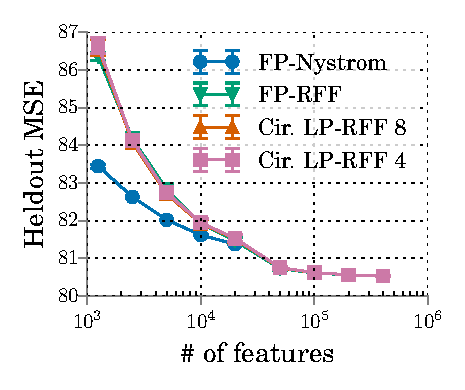
\includegraphics[width=0.3\linewidth]{figures/yearpred_MSE_vs_n_feat.pdf} &
%		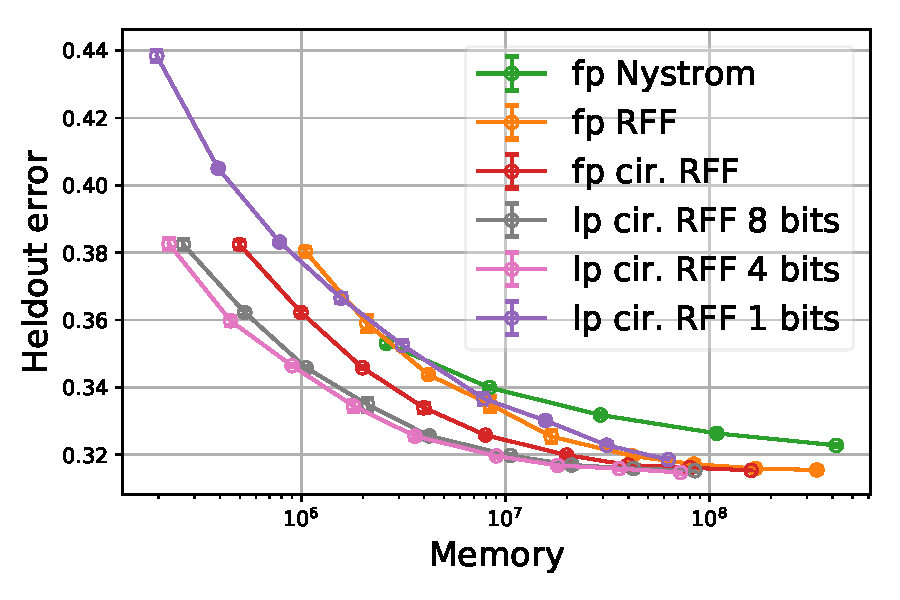
\includegraphics[width=0.3\linewidth]{figures/timit_error_vs_n_memory.pdf} &
%		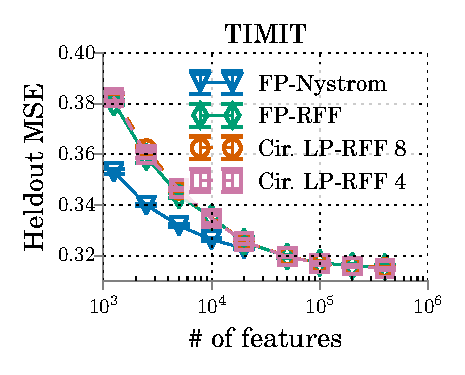
\includegraphics[width=0.3\linewidth]{figures/timit_error_vs_n_feat.pdf} \\
%		(a) Census & (b) YearPred & (c) Covtype & (d) TIMIT \\
%		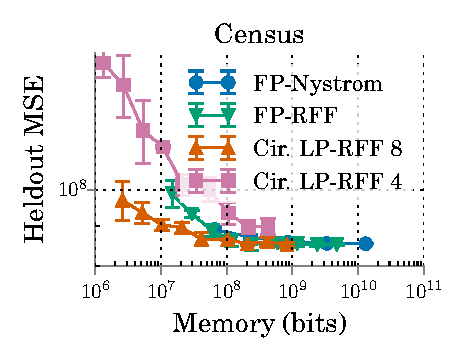
\includegraphics[width=0.3\linewidth]{figures/census_MSE_vs_n_memory.pdf} &
%		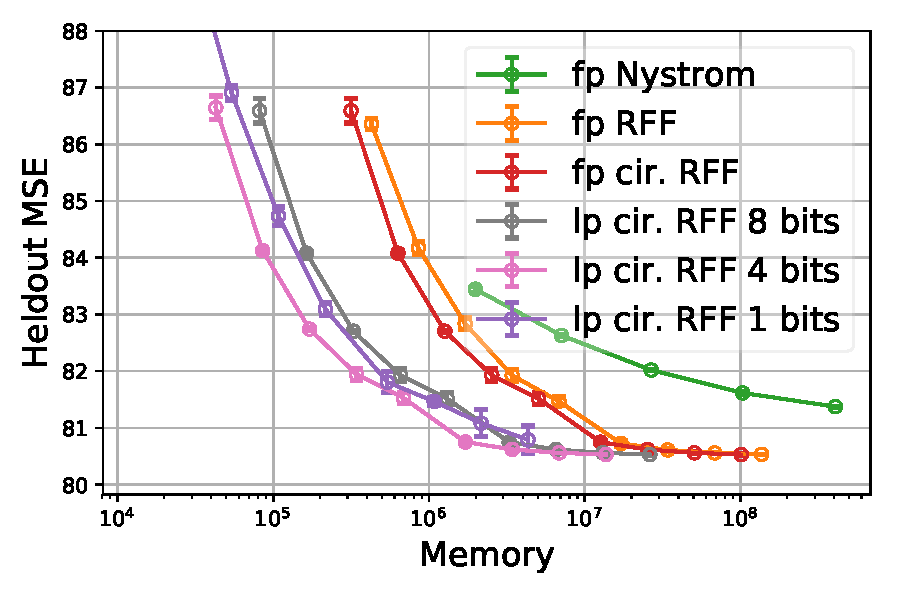
\includegraphics[width=0.3\linewidth]{figures/yearpred_MSE_vs_n_memory.pdf} &
%		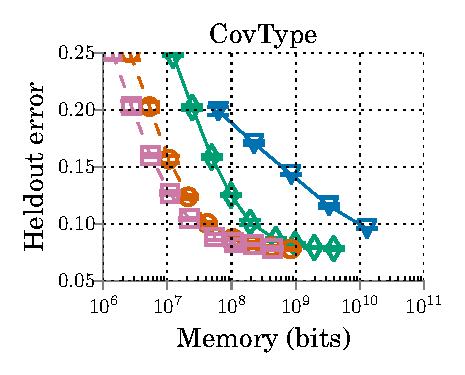
\includegraphics[width=0.3\linewidth]{figures/covtype_error_vs_n_memory.pdf} &
%		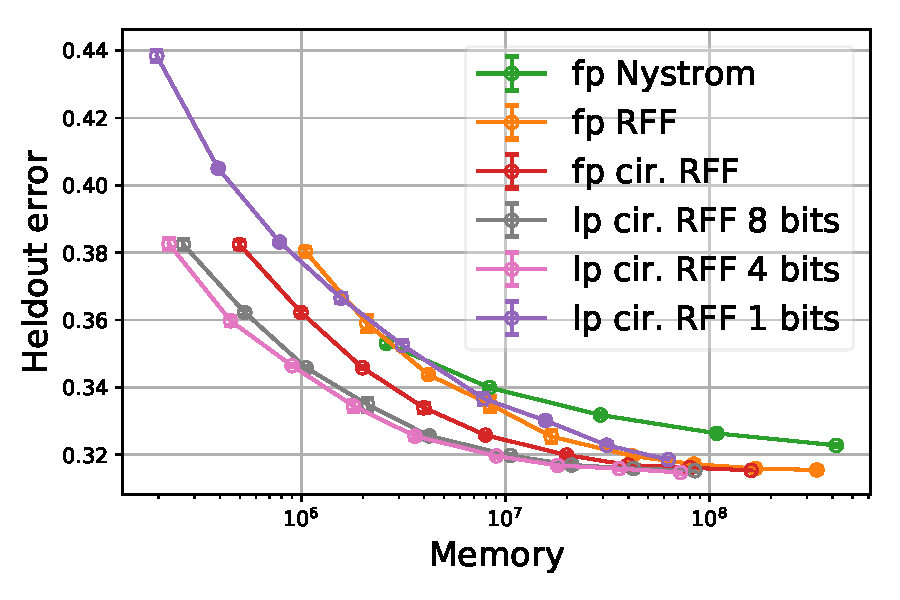
\includegraphics[width=0.3\linewidth]{figures/timit_error_vs_n_memory.pdf} \\
%		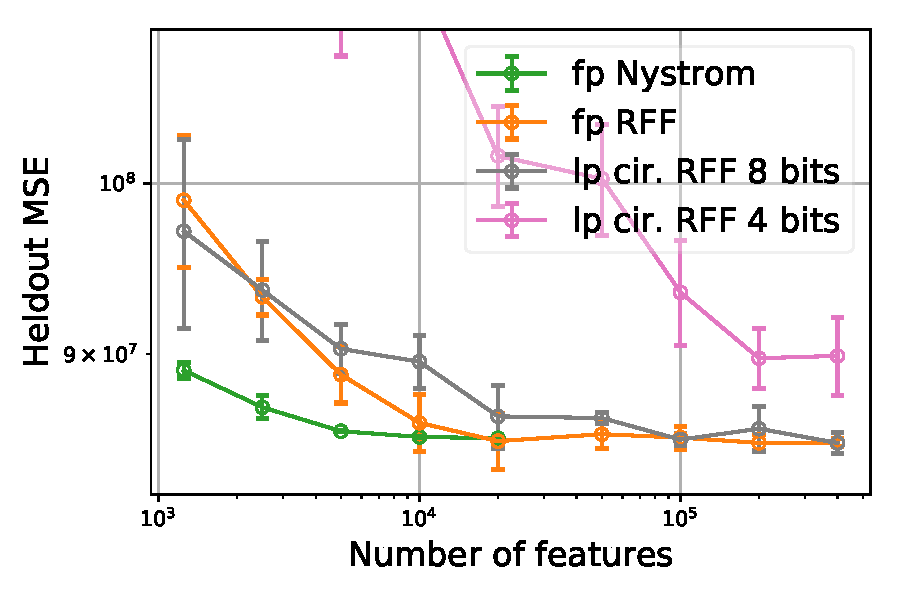
\includegraphics[width=0.3\linewidth]{figures/census_MSE_vs_n_feat.pdf} &
%		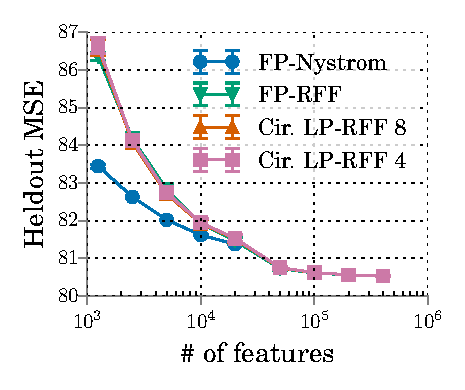
\includegraphics[width=0.3\linewidth]{figures/yearpred_MSE_vs_n_feat.pdf} &
%		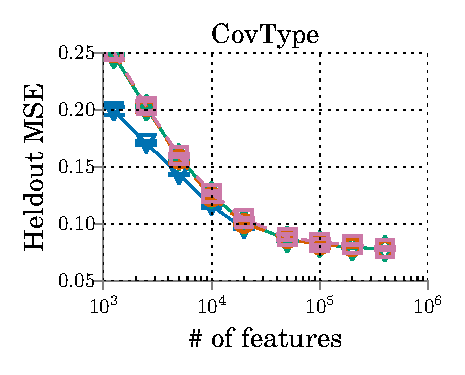
\includegraphics[width=0.3\linewidth]{figures/covtype_error_vs_n_feat.pdf} &
%		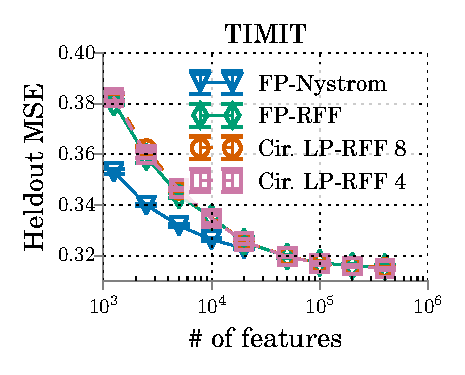
\includegraphics[width=0.3\linewidth]{figures/timit_error_vs_n_feat.pdf} \\
%		(a) Census & (b) YearPred & (c) Covtype & (d) TIMIT \\
	\end{tabular}
	\end{small}
	\caption{Generalization performance of LP-RFFs, FP-RFFs, and \Nystrom with respect to memory budgets (top) and number of features (bottom), on TIMIT and YearPred datasets.  LP-RFFs demonstrate better generalization performance than the full precision methods, under a memory budget. It is also informative to observe that while the \Nystrom method attains the best generalization performance with respect to the number of features, it is the worst performance method as a function of memory.
	For results on the CovType and Census datasets, please see Figure~\ref{fig:generalization_col_app} in Appendix~\ref{sec:exp_details}
}
	\label{fig:generalization_col}
\end{figure}

%% version with out model memory
%\begin{table}
%	\centering
%	\begin{tabular}{c c c c}
%		\hline
%		& FP RFF & FP circulant RFF & \Nystrom \\
%		\hline
%		\hline
%		Census & 5.56x & 30.32x & 122.52x \\
%		YearPred & 19.35x & 14.30x & 829.15x \\ 
%		Covtype & 9.17x & 7.57x & 460.80x \\ 
%		TIMIT & 70.42x & 25.68x & 843.41x \\ 
%		\hline
%	\end{tabular}
%	\caption{The memory savings from LP RFF to achieve within $1e^{-4}$ relative difference from the best generalization performance of baselines. We measure heldout L2 loss and heldout accuracy as the generalization performance respectively for regression and classification problems.}
%	\label{fig:mem_saving}
%\end{table}

% version with model memory
\begin{table}[ht]
\begin{minipage}{.6\linewidth}
\centering
	\begin{tabular}{c c c c}
		\hline
		& FP-RFFs & Cir. FP-RFFs & \Nystrom \\
		\hline
		\hline
%		Census & 2.8x / 1.13x & 30.7x / 7.7x & 62.2x / 4.09x \\
%		YearPred & 10.0x / 7.3x & 14.7x / 10.8x & 436.9x / 78.0x \\ 
%		Covtype & 4.6x / 4.6x & 7.6x / 7.6x & 230.4x / 75.3x \\ 
%		TIMIT & 5.1x / 2.0x & 3.9x / 3.6x & 50.6x / 8.9x \\ 
%		Census & 2.9x / 1.15x & 15.6x / 3.9x & 63.2x / 4.2x \\
%		YearPred & 10.3x / 7.7x & 7.6x / 5.7x & 461.6x / 80.3x \\ 
%		Covtype & 4.7x / 4.7x & 3.9x / 3.9x & 237.2x / 77.5x \\ 
%		TIMIT & 5.1x / 2.0x & 2.4x / 2.2x & 50.9x / 8.9x \\ 
		Census & 2.9x & 15.6x & 63.2x \\
		YearPred & 10.3x & 7.6x & 461.6x \\ 
		Covtype & 4.7x & 3.9x & 237.2x \\ 
		TIMIT & 5.1x & 2.4x & 50.9x \\ 
		\hline
	\end{tabular}
	\caption{The compression ratios achieved by LP-RFF relative to the best performing configurations for each baseline (FP-RFFs, circulant FP-RFFs, \NystromNS). For each baseline method, we find the best performing configuration as the reference performance, then record the memory consumption of the smallest LP-RFF and baseline models that are within $10^{-4}$ relative performance to this reference. The memory saving is reported as the ratio between the two recorded memory consumption.}
	\label{tab:mem_saving}
\end{minipage}
\begin{minipage}{0.05\linewidth}	
\end{minipage}
\begin{minipage}{0.35\linewidth}
	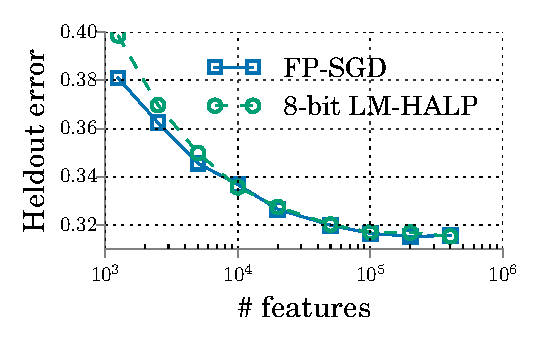
\includegraphics[width=\linewidth]{figures/timit_error_vs_n_feat_lm_halp.pdf}
	\caption{figure}{Low precision training using 8-bit HALP on TIMIT using 8-bit LP RFFs. Low precision training with HALP can demonstrate similar generalization performance as full precision training with SGD.}	
	\label{fig:halp}
\end{minipage}
\end{table}


\subsubsection{Low precision training for LP-RFFs}
\label{sec:halp}
In this section, we demonstrate that LP-RFFs can be trained using 8-bit low precision HALP training algorithm. The generalization performance from 8-bit HALP training can closely match the performance from full-precision SGD training. We use the same learning rate schedule as the one in the SGD-based experiments. We sweep the $\mu$ parameter, which determines the value of the quantization scale in HALP, using grid search over $\{0.001, 0.01, 0.1, 1.0\}$. For each number of LP-RFFs $m$, we choose the value of $\mu$ attaining lowest heldout classification error, and report this as the error. In Figure~\ref{fig:halp}, we can see that for 8-bit LP-RFFs, the generalization performance of the models trained with HALP can closely match the results from full-precision SGD, once the number of features exceed 10k. This shows, in scenarios where large numbers of kernel approximation features are required, we can safely train LP-RFFs with low precision training algorithms to reduce the memory footprint of training.
%\label{sec:lptrain}
%\begin{figure}
%\centering
%	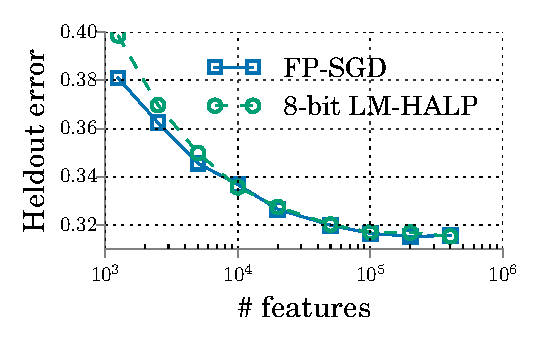
\includegraphics[width=.6\linewidth]{figures/timit_error_vs_n_feat_lm_halp.pdf}
%\label{fig:halp}
%\caption{Low precision training using HALP can demonstrate similar generalization performance as full precision training with SGD.}	
%\end{figure}

\subsection{Heldout performance vs. relative spectral distance}
In this section, our goal is to dig deeper into the strong generalization performance of LP-RFFs, by seeing whether these results can be understood in terms of the theory presented in Sections \ref{sec:genbound} and \ref{sec:lprff}.  In particular, the theory we presented bounds the generalization performance of the kernel approximation models using the relative spectral distance between the kernel approximation matrix, and the exact kernel matrix.  Although the theory as presented only applies to fixed design linear regression, in this section we ask whether relative spectral distance is predictive of generalization performance for non-fixed design kernel ridgre regression, as well as for kernel logistic regression.

We run experiments on the Census dataset, as well as on a sub-sampled version of the CovType dataset, where we select $20k$ training and heldout points at random.  The reason we use these smaller datasets is because computing the relative spectral distance is an expensive operation, which requires instantiating the kernel matrices fully, and performing singular value decompositions, which are expensive operations. For the Census dataset, we use the closed form solution for the kernel ridge regression estimator.  For CovType, because there is no closed form solution for logistic regression, we train the models with SGD using mini-batches of size 250; we pick the best initial learning rate, as well as regularization parameter, by using $20k$ \Nystrom features as a proxy for the exact kernel (note that because there are only $20k$ training points, this \Nystrom approximation is exact). For CovType, we pick the initial learning rate from the set $\{5, 10, 50, 100\}$, and for both tasks we pick the regularization parameter $\lambda \in \{1e^{-5}, 5e^{-5}, 1e^{-4}, 1e^{-3}, 5e^{-3}, 1e^{-2}, 5e^{-2}, 1e^{-1}\}$ which gives the best performance on the heldout set. We report the average $D_{\lambda}(K,\tK)$ and the average generalization performance, along with standard deviations, using 5 different random seeds.

In Figure~\ref{fig:specdist} (leftmost plots), we observe that LP-RFFs can achieve significantly smaller relative spectral distance $D_{\lambda}(K,\tK)$ than FP-RFFs and the \Nystrom method. Specifically, the 8 bit and 4 bit versions of LP-RFF attain the best relative spectral distance for Census and Covtype respectively. In this figure, we also show generalization performance vs. relative spectral distance (middle), as well as vs. the Frobenius norm of $K-\tK$ (right).  We can see that there is a strong correspondence between relative spectral distance and generalization performance across these methods, whereas for the Frobenius norm, the $\Nystrom$ method does not align well with the RFF-based methods. We observe a similar result with the spectral norm, and include these results in Appendix \todo{X}.

\begin{figure}
	\centering
%	\begin{tabular}{c c c}
%		\subfigure[MSE and relative spectral distance]{\label{fig:census_delta} 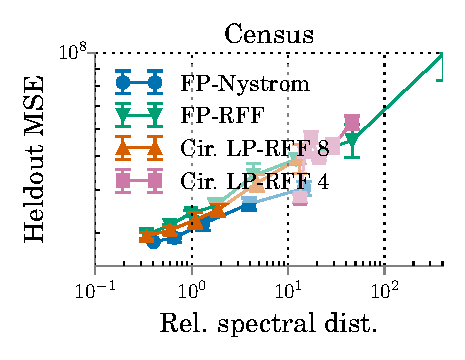
\includegraphics[width=0.33\linewidth]{figures/regression_l2_vs_delta.pdf} } \hfill
%		\subfigure[MSE and Frobenius norm]{\label{fig:census_f_norm} 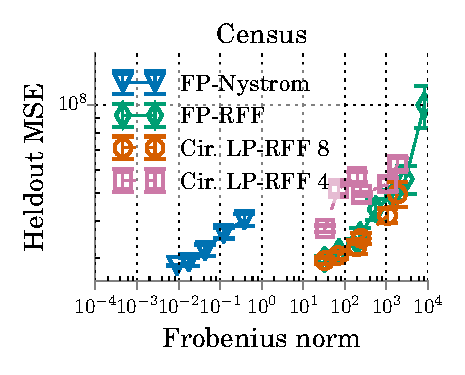
\includegraphics[width=0.33\linewidth]{figures/regression_l2_vs_f_norm.pdf} } \hfill
%		\subfigure[relative spectral distance and memory]{\label{fig:census_s_norm}  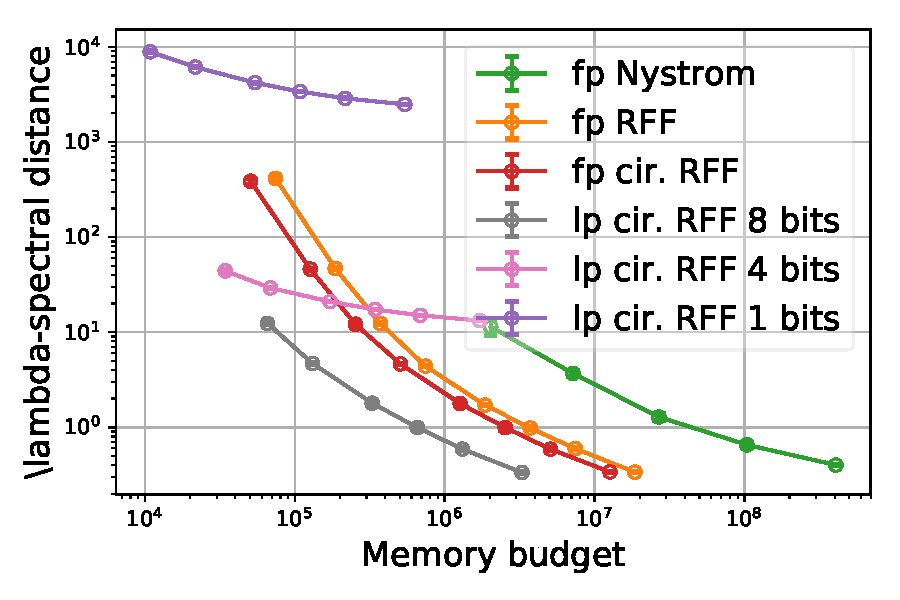
\includegraphics[width=0.33\linewidth]{figures/regression_delta_vs_mem.pdf} } \hfill \\
%		\subfigure[MSE and relative spectral distance]{\label{fig:covtype_delta} 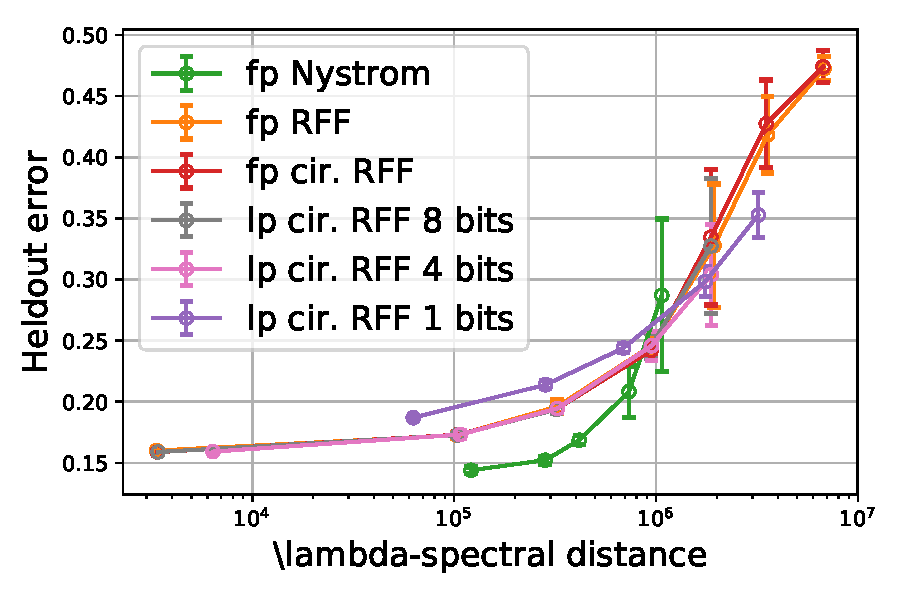
\includegraphics[width=0.33\linewidth]{figures/classification_acc_vs_delta.pdf} } \hfill
%		\subfigure[Error and Frobenius norm]{\label{fig:covtype_f_norm} 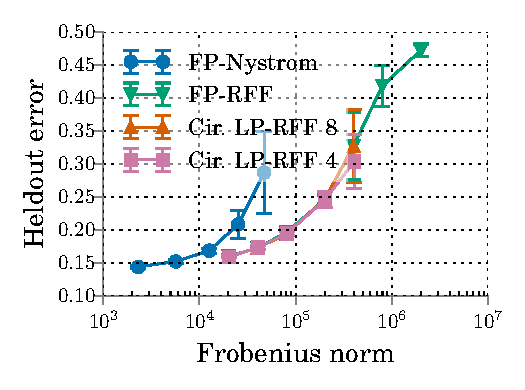
\includegraphics[width=0.33\linewidth]{figures/classification_acc_vs_f_norm.pdf} } \hfill
%		\subfigure[relative spectral distance and memory]{\label{fig:covtype_s_norm} 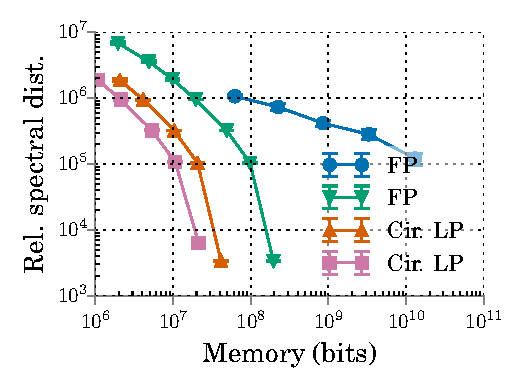
\includegraphics[width=0.33\linewidth]{figures/classification_delta_vs_mem.pdf}} \hfill
	\begin{tabular}{@{\hskip -0.1in}c@{\hskip -0.1in}c@{\hskip -0.1in}c@{\hskip -0.1in}}
		\subfigure[Census: $D_{\lambda}(K,\tK)$ vs. memory]{\label{fig:census_s_norm}  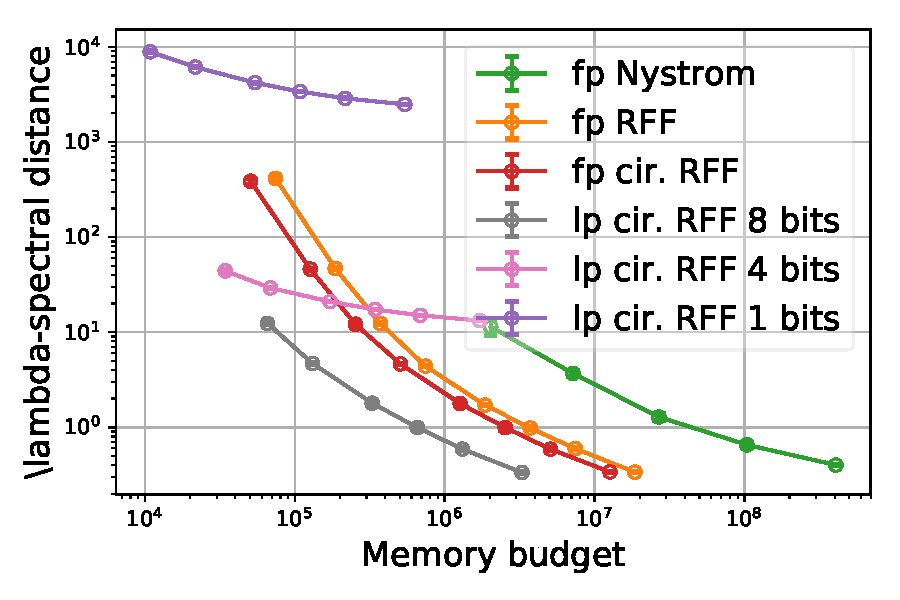
\includegraphics[width=0.33\linewidth]{figures/regression_delta_vs_mem.pdf} } \hfill 
		\subfigure[Census: MSE vs. $D_{\lambda}(K,\tK)$]{\label{fig:census_delta} 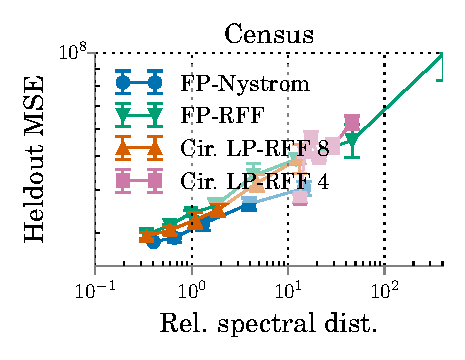
\includegraphics[width=0.33\linewidth]{figures/regression_l2_vs_delta.pdf} } \hfill
		\subfigure[Census: MSE vs. Frob. norm]{\label{fig:census_f_norm} 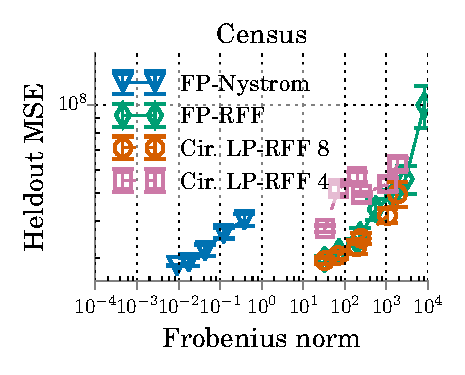
\includegraphics[width=0.33\linewidth]{figures/regression_l2_vs_f_norm.pdf} } \hfill \\
		\subfigure[CovType: $D_{\lambda}(K,\tK)$ vs. mem.]{\label{fig:covtype_s_norm} 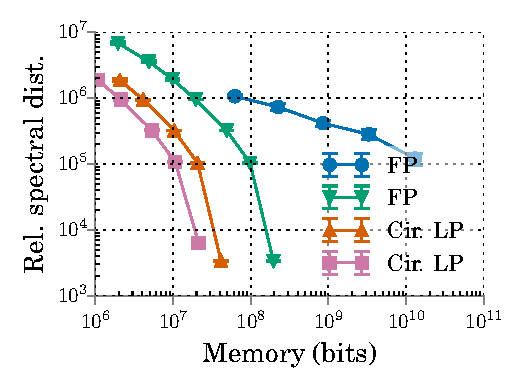
\includegraphics[width=0.33\linewidth]{figures/classification_delta_vs_mem.pdf}} \hfill
		\subfigure[CovType: MSE vs. $D_{\lambda}(K,\tK)$]{\label{fig:covtype_delta} 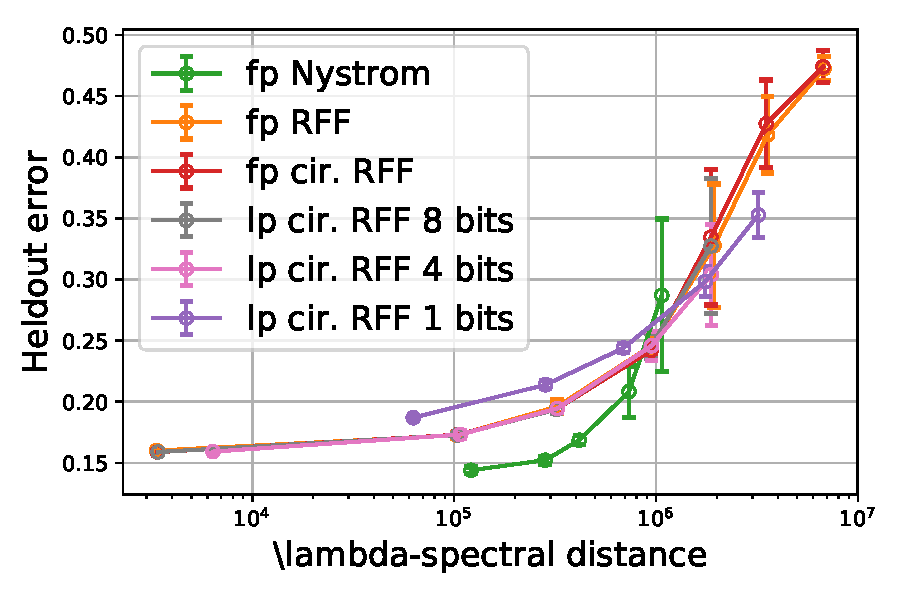
\includegraphics[width=0.33\linewidth]{figures/classification_acc_vs_delta.pdf} } \hfill
		\subfigure[CovType: Error vs. Frob. norm]{\label{fig:covtype_f_norm} 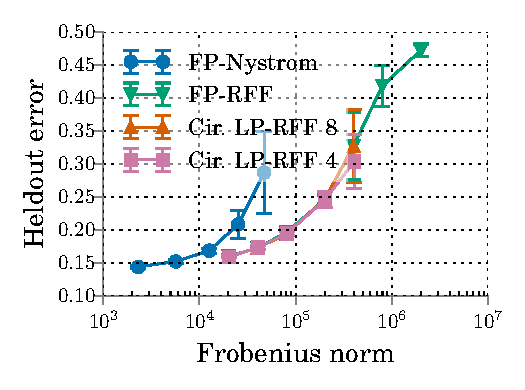
\includegraphics[width=0.33\linewidth]{figures/classification_acc_vs_f_norm.pdf} } \hfill
	\end{tabular}
	\caption{Analysis of generalization performance for Census and sub-sampled CovType. We measure the relative spectral distance $D_{\lambda}(K,\tK)$ for LP-RFFs, FP-RFFs, and \Nystrom, as a function of the memory utilization, and observe that LP-RFFs attain lower relative spectral distance per bit (rightmost plot). We then plot generalization performance as a function of relative spectral distance (middle), and Frobenius norm of $K - \tK$ (right). We observe a tigher correspondance between the generalization performance and relative spectral distance, relative to the Frobenius norm, on both datasets.}
	\label{fig:specdist}
\end{figure}

%\begin{figure}
%	\centering
%	\begin{tabular}{c c c}
%		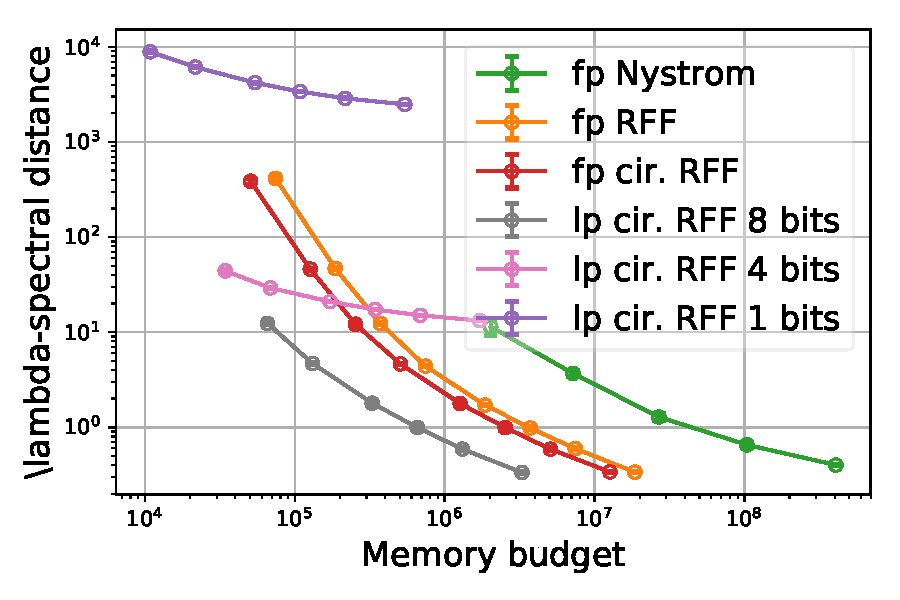
\includegraphics[width=0.33\linewidth]{figures/regression_delta_vs_mem.pdf} &
%		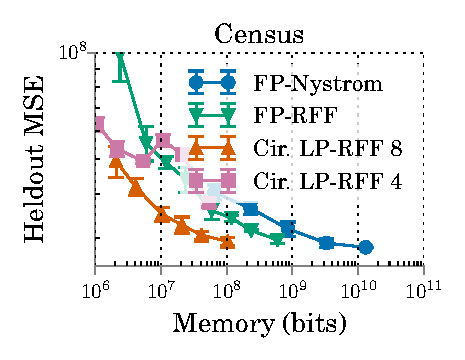
\includegraphics[width=0.33\linewidth]{figures/regression_l2_vs_mem.pdf} &
%		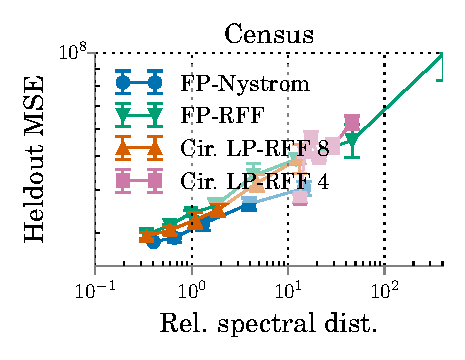
\includegraphics[width=0.33\linewidth]{figures/regression_l2_vs_delta.pdf} \\
%		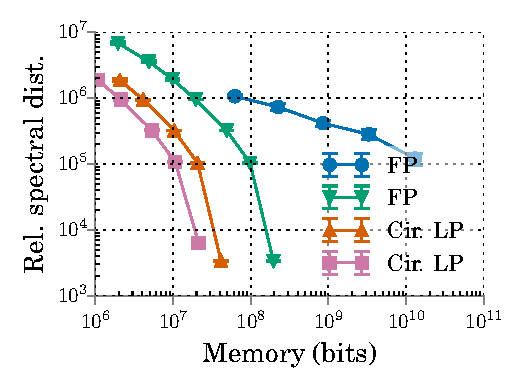
\includegraphics[width=0.33\linewidth]{figures/classification_delta_vs_mem.pdf} &
%		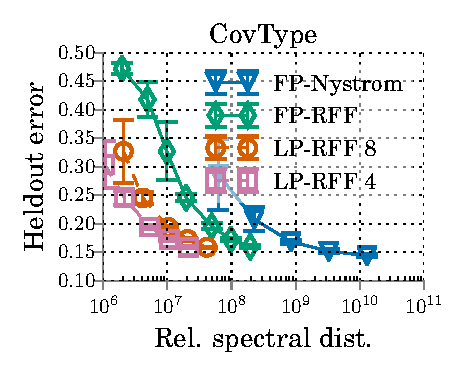
\includegraphics[width=0.33\linewidth]{figures/classification_acc_vs_mem.pdf} &
%		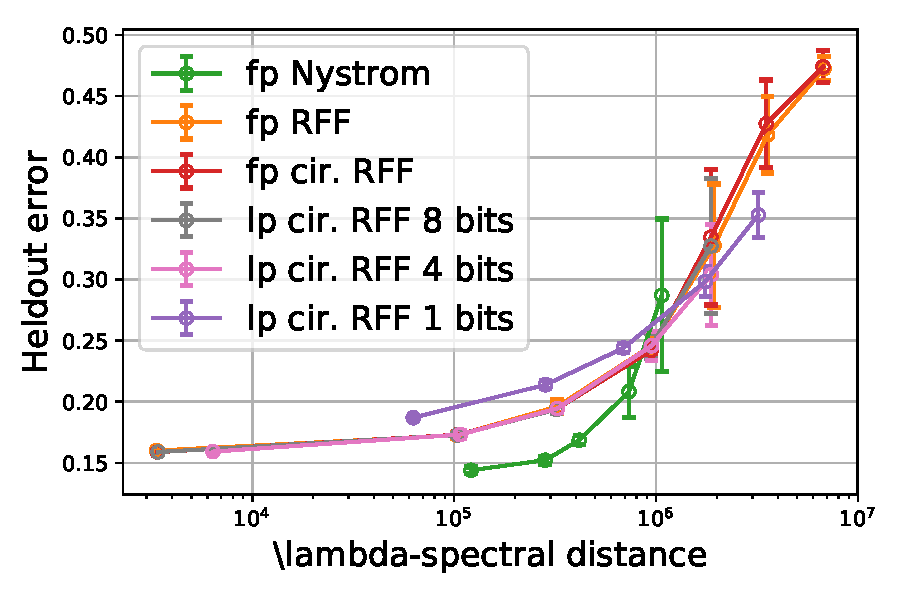
\includegraphics[width=0.33\linewidth]{figures/classification_acc_vs_delta.pdf} \\
%		(a) & (b) & (c)
%	\end{tabular}
%	\caption{The strong correlation between generalization performance and relative spectral distance $D_{\lambda}(K,\tK)$ under memory budgets for the Census dataset (top) and subsampled CovType dataset (bottom). Under different memory budget in (a) and (b), the precision demonstrates smaller $D_{\lambda}(K,\tK)$ tends to have better generalization performance. In (c), different kernel approximation approaches demonstrate similar generalization performance for similar relative spectral distance.}
%	\label{fig:specdist}
%\end{figure}



%(z_x+\teps_x)(z_y+\teps_y)$, where $\teps_x \sim X_{z_x}^{-\sq,\sq}$, and $\teps_y \sim X_{z_y}^{-\sq,\sq}$.
%Then $\var{}{\tS} = 4 - z_x^2 z_y^2$.
\section{References}
\noindent$[1]$ Large Scale Kernel Learning using Block Coordinate Descent.
Stephen Tu, Rebecca Roelofs, Shivaram Venkataraman, Benjamin Recht. \url{https://arxiv.org/pdf/1602.05310.pdf}. \\
$[2]$ CoCoA: A General Framework for Communication-Efficient Distributed Optimization.
Virginia Smith, Simone Forte, Chenxin Ma, Martin Takac, Michael I. Jordan, Martin Jaggi.  \url{https://arxiv.org/abs/1611.02189} \\
$[3]$ On the Error of Random Fourier Features. Dougal J. Sutherland, Jeff Schneider. UAI 2015. \url{https://arxiv.org/abs/1506.02785}\\
$[4]$ Weighted Sums of Random Kitchen Sinks: Replacing minimization with randomization in learning. Ali Rahimi, Ben Recht. NIPS 2008.\\
$[5]$	Random Features for Large-Scale Kernel Machines. Ali Rahimi, Benjamin Recht. NIPS 2007:
\end{document}


\section{Experiments}
\label{sec:experiments}
In this section, we compare the performance of LP-RFFs with full-precision RFFs (FP-RFFs), circulant FP-RFFs, and the \Nystrom method, on the TIMIT, YearPred, CovType, and Census datasets, showing that we can attain compression ratios of at least 2.4x relative to these methods, without hurting generalization performance. We then perform a more careful analysis of these results on the Census dataset and a sub-sampled version of the CovType dataset, where we plot the generalization performance of these approximation methods relative to their relative spectral distances. We observe on both datasets that the relative spectral distance appears much more predictive of generalization performance than more standard metrics like the Frobenius and spectral norms of $K-\tK$.  We note that in our experiments, in order to avoid the risk of numerical precision issues (kernel ridge regression requires matrix inversion), we do all our full-precision experiments in 64 bits.  Nonetheless, we calculate the memory utilization of these experiments as if we used 32 bits, to avoid inflating the relative gains of our method over the full precision approaches.

For all our experiments, we use the Gaussian kernel with the kernel width value recommended by~\citet{may2017}, and compute the memory utilization as described in Section~\ref{subsec:memory_utils}. To evaluate the performance of these kernel models, we measure the classification error for classification tasks, and the mean squared error (MSE) for regression tasks ($\frac{1}{n}\sum_{i=1}^n (f_{\tK}(x_i) - y_i)^2$), on the heldout set. We include more details about our datasets, experimental protocols, and hyperparameter choices in Appendix~\ref{sec:exp_details}.

\subsection{Empirical evaluation of LP-RFFs}
We compare the generalization performance of LP-RFFs to FP-RFFs, circulant FP-RFFs, and \Nystrom features, across four datasets, for various memory budgets.  We sweep the following hyperparameters: For LP-RFFs, we choose the precision $b \in \{1,2,4,8,16\}$. For \NystromNS, we use $m \in \{1250, 2500, 5000, 10000, 20000\}$.  For the RFF-based methods, we use $m\in \{1250, 2500, 5000, 10000, 20000, 50000, 100000, 200000, 400000\}$. We choose these limits differently because $\num[group-separator={,}]{20000}$ \Nystrom features have roughly the same memory footprint as $\num[group-separator={,}]{400000}$ FP-RFFs. For all experiments, we use a mini-batch size of $250$. We avoid the prohibitively large computational expense of performing a grid search to tune the initial learning rate, the regularizer, the learning rate decay, and the number of training epochs, by using the heldout set in order to determine learning rate decay \citep{morgan1990generalization,sainath2013b,sainath2013low}. The scheme works as follows: at the end of each epoch, we decay the learning rate in half if the heldout performance is less than $1\%$ better relative to the previous best model, using MSE for regression and cross entropy for classification. Furthermore, if the model performs \textit{worse} than the previous best, we revert the model. The training terminates after the learning rate has been decayed 10 times. Early stopping can be seen as a form of regularization \citep{zhang2005boosting,wei2017early}.  We use a single initial learning rate per dataset across all experiments, which we tune via grid search using $20\text{k}$ \Nystrom features. We choose to use \Nystrom features to tune the initial learning rate in order to avoid biasing the results in favor of RFF-based approaches. 

In Figure \ref{fig:generalization_col}, we plot the generalization performance for all these experiments, as a function of the amount of memory used, as well as the number of features $m$. We show across all four datasets that LP-RFFs show systematically better generalization performance than the full precision baselines under various memory budgets. Importantly, we see that the \Nystrom method has observably better generalization performance than LP-RFF and FP-RFF-based baselines under the same number of features. However, when we instead consider performance as a function of memory utilization, the opposite it true, with the RFF-based methods demonstrating superior generalization performance. This observation further validates the practical importance of comparing kernel approximation methods under memory budgets.

In Table~\ref{tab:mem_saving} we present the compression ratios we achieve with LP-RFFs, relative to the baselines, while still attaining generalization performance within $10^{-4}$ of the full-precision baseline.  We measure this as follows: For each baseline (FP-RFFs, circulant FP-RFFs, \Nystrom), we find the best performing (as well as median) model. We then find the smallest LP-RFF model, as well as the smallest baseline model, which attains within $10^{-4}$ relative performance to the best performing baseline.  We report the ratio of the memory used by these two models (baseline/LP-RFF), that are both within $10^{-4}$ of the best baseline. We compute this ratio across three independent runs using different random seeds, and report the average.  We can see that LP-RFFs demonstrate significant memory saving over FP-RFFs and circulant FP-RFFs, showing 2.9x-10.3x and 2.4x-15.6x compression ratios respectively. On the TIMIT dataset, there are 147 classes, and thus the full-precision learned parameters occupy a large portion of the total memory across all methods. Nonetheless, even though these LP-RFF experiments only quantize the feature mini-batches, they still attain 5.1x and 2.4x compression ratios relative to FP-RFF and circulant FP-RFF.

\begin{figure}
	\centering
	\begin{small}
	\begin{tabular}{@{\hskip -0.05in}c@{\hskip -0.1in}c@{\hskip -0.1in}c@{\hskip -0.1in}c@{\hskip -0.05in}}
%		\subfigure[YearPred MSE vs. Mem.]{\label{fig:year_pred_mem} 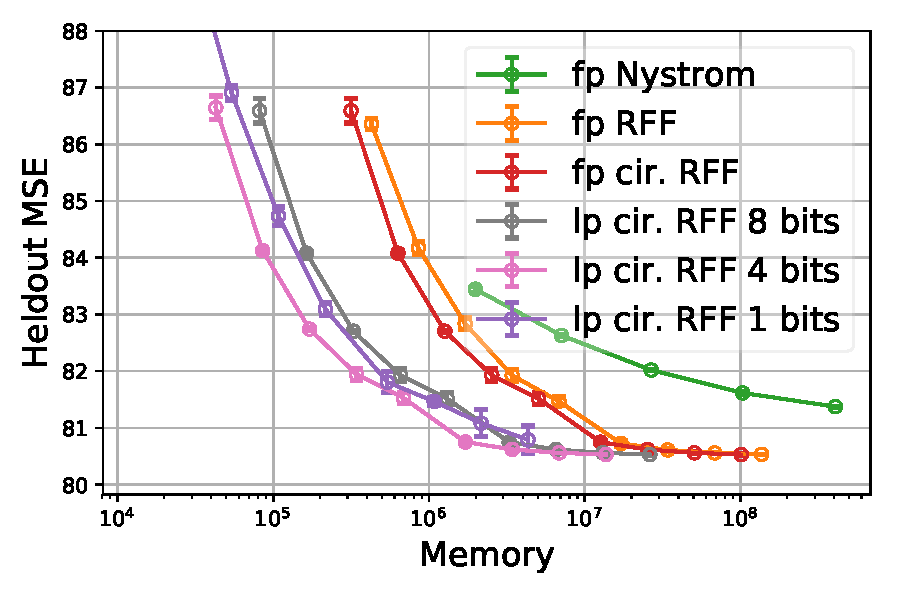
\includegraphics[width=0.27\linewidth]{figures/yearpred_MSE_vs_n_memory.pdf} } \hfill
%		\subfigure[TIMIT Err. vs. Mem.]{\label{fig:year_pred_mem} 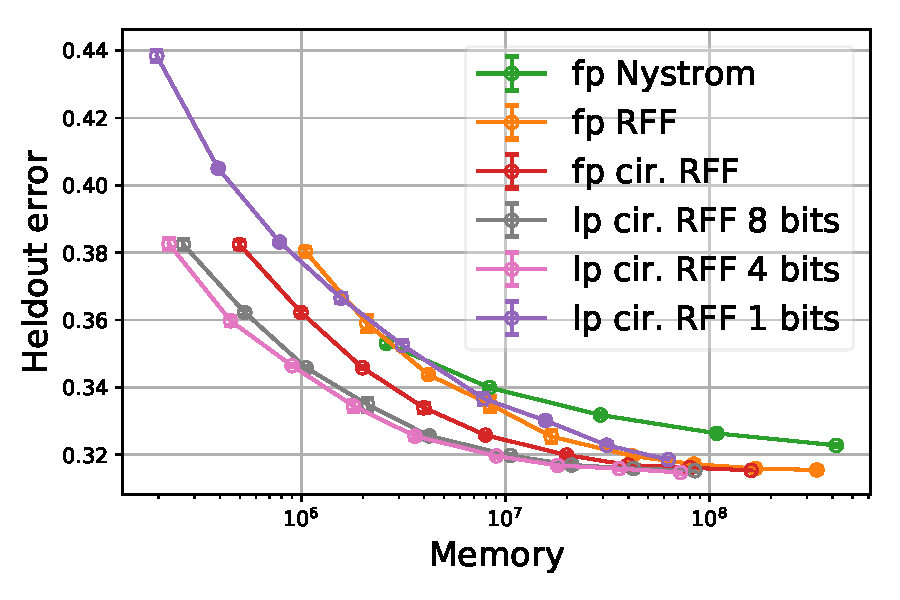
\includegraphics[width=0.27\linewidth]{figures/timit_error_vs_n_memory.pdf} } \hfill
%		\subfigure[YearPred MSE vs. Feat.]{\label{fig:year_pred_feat}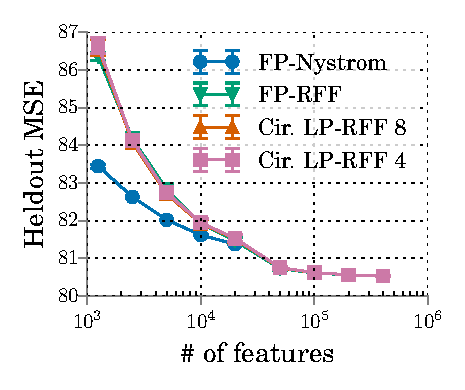
\includegraphics[width=0.27\linewidth]{figures/yearpred_MSE_vs_n_feat.pdf} } \hfill
%		\subfigure[TIMIT Err vs. Feat.]{\label{fig:year_pred_feat}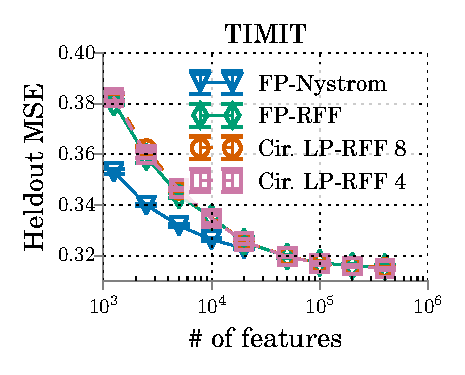
\includegraphics[width=0.27\linewidth]{figures/timit_error_vs_n_feat.pdf} } \hfill
		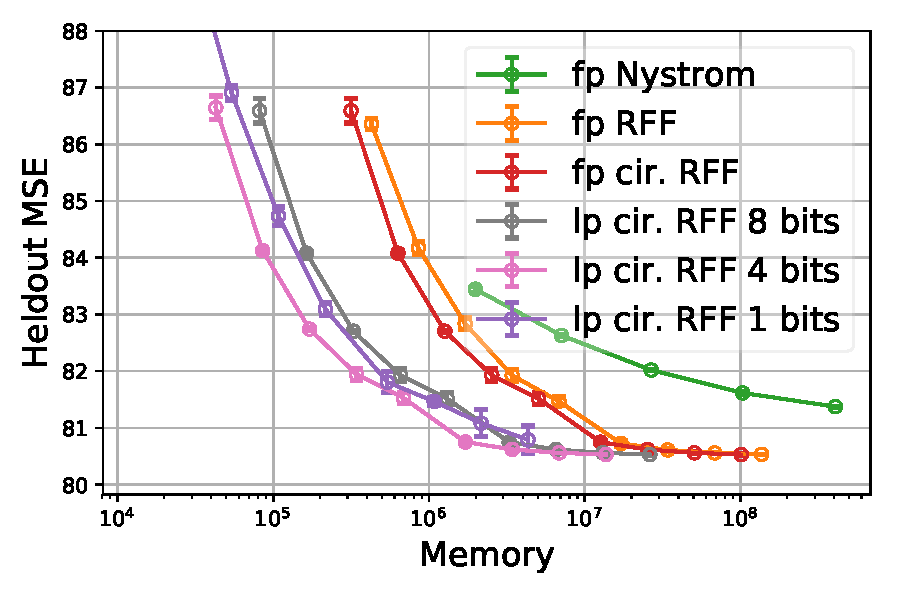
\includegraphics[width=0.27\linewidth]{figures/yearpred_MSE_vs_n_memory.pdf} &
		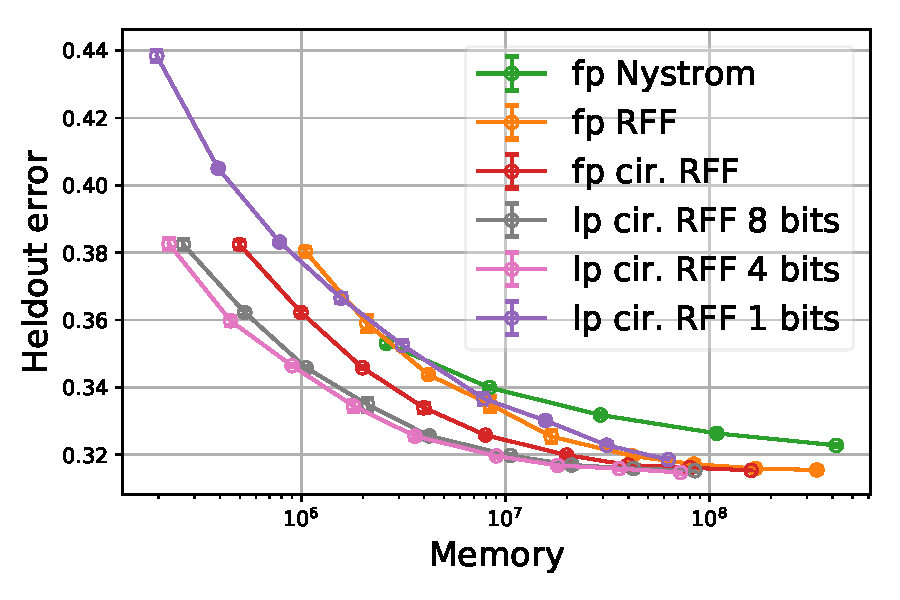
\includegraphics[width=0.27\linewidth]{figures/timit_error_vs_n_memory.pdf} &
		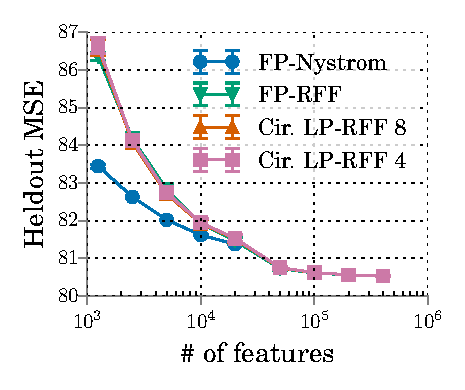
\includegraphics[width=0.27\linewidth]{figures/yearpred_MSE_vs_n_feat.pdf} &
		\includegraphics[width=0.27\linewidth]{figures/timit_error_vs_n_feat.pdf} \\
		(a) YearPred MSE vs. Mem. & (b) TIMIT Err. vs. Mem. & (c) YearPred MSE vs. Feat. & (d) TIMIT Err vs. Feat.\\
%		\includegraphics[width=0.3\linewidth]{figures/yearpred_MSE_vs_n_memory.pdf} &
%		\includegraphics[width=0.3\linewidth]{figures/yearpred_MSE_vs_n_feat.pdf} &
%		\includegraphics[width=0.3\linewidth]{figures/timit_error_vs_n_memory.pdf} &
%		\includegraphics[width=0.3\linewidth]{figures/timit_error_vs_n_feat.pdf} \\
%		(a) Census & (b) YearPred & (c) Covtype & (d) TIMIT \\
%		\includegraphics[width=0.3\linewidth]{figures/census_MSE_vs_n_memory.pdf} &
%		\includegraphics[width=0.3\linewidth]{figures/yearpred_MSE_vs_n_memory.pdf} &
%		\includegraphics[width=0.3\linewidth]{figures/covtype_error_vs_n_memory.pdf} &
%		\includegraphics[width=0.3\linewidth]{figures/timit_error_vs_n_memory.pdf} \\
%		\includegraphics[width=0.3\linewidth]{figures/census_MSE_vs_n_feat.pdf} &
%		\includegraphics[width=0.3\linewidth]{figures/yearpred_MSE_vs_n_feat.pdf} &
%		\includegraphics[width=0.3\linewidth]{figures/covtype_error_vs_n_feat.pdf} &
%		\includegraphics[width=0.3\linewidth]{figures/timit_error_vs_n_feat.pdf} \\
%		(a) Census & (b) YearPred & (c) Covtype & (d) TIMIT \\
	\end{tabular}
	\end{small}
	\caption{Generalization performance of LP-RFFs, FP-RFFs, and \Nystrom with respect to memory budgets (top) and number of features (bottom), on TIMIT and YearPred datasets.  LP-RFFs demonstrate better generalization performance than the full precision methods, under a memory budget. It is also informative to observe that while the \Nystrom method attains the best generalization performance with respect to the number of features, it is the worst performance method as a function of memory.
	For results on the CovType and Census datasets, please see Figure~\ref{fig:generalization_col_app} in Appendix~\ref{sec:exp_details}
}
	\label{fig:generalization_col}
\end{figure}

%% version with out model memory
%\begin{table}
%	\centering
%	\begin{tabular}{c c c c}
%		\hline
%		& FP RFF & FP circulant RFF & \Nystrom \\
%		\hline
%		\hline
%		Census & 5.56x & 30.32x & 122.52x \\
%		YearPred & 19.35x & 14.30x & 829.15x \\ 
%		Covtype & 9.17x & 7.57x & 460.80x \\ 
%		TIMIT & 70.42x & 25.68x & 843.41x \\ 
%		\hline
%	\end{tabular}
%	\caption{The memory savings from LP RFF to achieve within $1e^{-4}$ relative difference from the best generalization performance of baselines. We measure heldout L2 loss and heldout accuracy as the generalization performance respectively for regression and classification problems.}
%	\label{fig:mem_saving}
%\end{table}

% version with model memory
\begin{table}[ht]
\begin{minipage}{.6\linewidth}
\centering
	\begin{tabular}{c c c c}
		\hline
		& FP-RFFs & Cir. FP-RFFs & \Nystrom \\
		\hline
		\hline
%		Census & 2.8x / 1.13x & 30.7x / 7.7x & 62.2x / 4.09x \\
%		YearPred & 10.0x / 7.3x & 14.7x / 10.8x & 436.9x / 78.0x \\ 
%		Covtype & 4.6x / 4.6x & 7.6x / 7.6x & 230.4x / 75.3x \\ 
%		TIMIT & 5.1x / 2.0x & 3.9x / 3.6x & 50.6x / 8.9x \\ 
%		Census & 2.9x / 1.15x & 15.6x / 3.9x & 63.2x / 4.2x \\
%		YearPred & 10.3x / 7.7x & 7.6x / 5.7x & 461.6x / 80.3x \\ 
%		Covtype & 4.7x / 4.7x & 3.9x / 3.9x & 237.2x / 77.5x \\ 
%		TIMIT & 5.1x / 2.0x & 2.4x / 2.2x & 50.9x / 8.9x \\ 
		Census & 2.9x & 15.6x & 63.2x \\
		YearPred & 10.3x & 7.6x & 461.6x \\ 
		Covtype & 4.7x & 3.9x & 237.2x \\ 
		TIMIT & 5.1x & 2.4x & 50.9x \\ 
		\hline
	\end{tabular}
	\caption{The compression ratios achieved by LP-RFF relative to the best performing configurations for each baseline (FP-RFFs, circulant FP-RFFs, \NystromNS). For each baseline method, we find the best performing configuration as the reference performance, then record the memory consumption of the smallest LP-RFF and baseline models that are within $10^{-4}$ relative performance to this reference. The memory saving is reported as the ratio between the two recorded memory consumption.}
	\label{tab:mem_saving}
\end{minipage}
\begin{minipage}{0.05\linewidth}	
\end{minipage}
\begin{minipage}{0.35\linewidth}
	\includegraphics[width=\linewidth]{figures/timit_error_vs_n_feat_lm_halp.pdf}
	\caption{figure}{Low precision training using 8-bit HALP on TIMIT using 8-bit LP RFFs. Low precision training with HALP can demonstrate similar generalization performance as full precision training with SGD.}	
	\label{fig:halp}
\end{minipage}
\end{table}


\subsubsection{Low precision training for LP-RFFs}
\label{sec:halp}
In this section, we demonstrate that LP-RFFs can be trained using 8-bit low precision HALP training algorithm. The generalization performance from 8-bit HALP training can closely match the performance from full-precision SGD training. We use the same learning rate schedule as the one in the SGD-based experiments. We sweep the $\mu$ parameter, which determines the value of the quantization scale in HALP, using grid search over $\{0.001, 0.01, 0.1, 1.0\}$. For each number of LP-RFFs $m$, we choose the value of $\mu$ attaining lowest heldout classification error, and report this as the error. In Figure~\ref{fig:halp}, we can see that for 8-bit LP-RFFs, the generalization performance of the models trained with HALP can closely match the results from full-precision SGD, once the number of features exceed 10k. This shows, in scenarios where large numbers of kernel approximation features are required, we can safely train LP-RFFs with low precision training algorithms to reduce the memory footprint of training.
%\label{sec:lptrain}
%\begin{figure}
%\centering
%	\includegraphics[width=.6\linewidth]{figures/timit_error_vs_n_feat_lm_halp.pdf}
%\label{fig:halp}
%\caption{Low precision training using HALP can demonstrate similar generalization performance as full precision training with SGD.}	
%\end{figure}

\subsection{Heldout performance vs. relative spectral distance}
In this section, our goal is to dig deeper into the strong generalization performance of LP-RFFs, by seeing whether these results can be understood in terms of the theory presented in Sections \ref{sec:genbound} and \ref{sec:lprff}.  In particular, the theory we presented bounds the generalization performance of the kernel approximation models using the relative spectral distance between the kernel approximation matrix, and the exact kernel matrix.  Although the theory as presented only applies to fixed design linear regression, in this section we ask whether relative spectral distance is predictive of generalization performance for non-fixed design kernel ridgre regression, as well as for kernel logistic regression.

We run experiments on the Census dataset, as well as on a sub-sampled version of the CovType dataset, where we select $20k$ training and heldout points at random.  The reason we use these smaller datasets is because computing the relative spectral distance is an expensive operation, which requires instantiating the kernel matrices fully, and performing singular value decompositions, which are expensive operations. For the Census dataset, we use the closed form solution for the kernel ridge regression estimator.  For CovType, because there is no closed form solution for logistic regression, we train the models with SGD using mini-batches of size 250; we pick the best initial learning rate, as well as regularization parameter, by using $20k$ \Nystrom features as a proxy for the exact kernel (note that because there are only $20k$ training points, this \Nystrom approximation is exact). For CovType, we pick the initial learning rate from the set $\{5, 10, 50, 100\}$, and for both tasks we pick the regularization parameter $\lambda \in \{1e^{-5}, 5e^{-5}, 1e^{-4}, 1e^{-3}, 5e^{-3}, 1e^{-2}, 5e^{-2}, 1e^{-1}\}$ which gives the best performance on the heldout set. We report the average $D_{\lambda}(K,\tK)$ and the average generalization performance, along with standard deviations, using 5 different random seeds.

In Figure~\ref{fig:specdist} (leftmost plots), we observe that LP-RFFs can achieve significantly smaller relative spectral distance $D_{\lambda}(K,\tK)$ than FP-RFFs and the \Nystrom method. Specifically, the 8 bit and 4 bit versions of LP-RFF attain the best relative spectral distance for Census and Covtype respectively. In this figure, we also show generalization performance vs. relative spectral distance (middle), as well as vs. the Frobenius norm of $K-\tK$ (right).  We can see that there is a strong correspondence between relative spectral distance and generalization performance across these methods, whereas for the Frobenius norm, the $\Nystrom$ method does not align well with the RFF-based methods. We observe a similar result with the spectral norm, and include these results in Appendix \todo{X}.

\begin{figure}
	\centering
%	\begin{tabular}{c c c}
%		\subfigure[MSE and relative spectral distance]{\label{fig:census_delta} \includegraphics[width=0.33\linewidth]{figures/regression_l2_vs_delta.pdf} } \hfill
%		\subfigure[MSE and Frobenius norm]{\label{fig:census_f_norm} \includegraphics[width=0.33\linewidth]{figures/regression_l2_vs_f_norm.pdf} } \hfill
%		\subfigure[relative spectral distance and memory]{\label{fig:census_s_norm}  \includegraphics[width=0.33\linewidth]{figures/regression_delta_vs_mem.pdf} } \hfill \\
%		\subfigure[MSE and relative spectral distance]{\label{fig:covtype_delta} \includegraphics[width=0.33\linewidth]{figures/classification_acc_vs_delta.pdf} } \hfill
%		\subfigure[Error and Frobenius norm]{\label{fig:covtype_f_norm} \includegraphics[width=0.33\linewidth]{figures/classification_acc_vs_f_norm.pdf} } \hfill
%		\subfigure[relative spectral distance and memory]{\label{fig:covtype_s_norm} \includegraphics[width=0.33\linewidth]{figures/classification_delta_vs_mem.pdf}} \hfill
	\begin{tabular}{@{\hskip -0.1in}c@{\hskip -0.1in}c@{\hskip -0.1in}c@{\hskip -0.1in}}
		\subfigure[Census: $D_{\lambda}(K,\tK)$ vs. memory]{\label{fig:census_s_norm}  \includegraphics[width=0.33\linewidth]{figures/regression_delta_vs_mem.pdf} } \hfill 
		\subfigure[Census: MSE vs. $D_{\lambda}(K,\tK)$]{\label{fig:census_delta} \includegraphics[width=0.33\linewidth]{figures/regression_l2_vs_delta.pdf} } \hfill
		\subfigure[Census: MSE vs. Frob. norm]{\label{fig:census_f_norm} \includegraphics[width=0.33\linewidth]{figures/regression_l2_vs_f_norm.pdf} } \hfill \\
		\subfigure[CovType: $D_{\lambda}(K,\tK)$ vs. mem.]{\label{fig:covtype_s_norm} \includegraphics[width=0.33\linewidth]{figures/classification_delta_vs_mem.pdf}} \hfill
		\subfigure[CovType: MSE vs. $D_{\lambda}(K,\tK)$]{\label{fig:covtype_delta} \includegraphics[width=0.33\linewidth]{figures/classification_acc_vs_delta.pdf} } \hfill
		\subfigure[CovType: Error vs. Frob. norm]{\label{fig:covtype_f_norm} \includegraphics[width=0.33\linewidth]{figures/classification_acc_vs_f_norm.pdf} } \hfill
	\end{tabular}
	\caption{Analysis of generalization performance for Census and sub-sampled CovType. We measure the relative spectral distance $D_{\lambda}(K,\tK)$ for LP-RFFs, FP-RFFs, and \Nystrom, as a function of the memory utilization, and observe that LP-RFFs attain lower relative spectral distance per bit (rightmost plot). We then plot generalization performance as a function of relative spectral distance (middle), and Frobenius norm of $K - \tK$ (right). We observe a tigher correspondance between the generalization performance and relative spectral distance, relative to the Frobenius norm, on both datasets.}
	\label{fig:specdist}
\end{figure}

%\begin{figure}
%	\centering
%	\begin{tabular}{c c c}
%		\includegraphics[width=0.33\linewidth]{figures/regression_delta_vs_mem.pdf} &
%		\includegraphics[width=0.33\linewidth]{figures/regression_l2_vs_mem.pdf} &
%		\includegraphics[width=0.33\linewidth]{figures/regression_l2_vs_delta.pdf} \\
%		\includegraphics[width=0.33\linewidth]{figures/classification_delta_vs_mem.pdf} &
%		\includegraphics[width=0.33\linewidth]{figures/classification_acc_vs_mem.pdf} &
%		\includegraphics[width=0.33\linewidth]{figures/classification_acc_vs_delta.pdf} \\
%		(a) & (b) & (c)
%	\end{tabular}
%	\caption{The strong correlation between generalization performance and relative spectral distance $D_{\lambda}(K,\tK)$ under memory budgets for the Census dataset (top) and subsampled CovType dataset (bottom). Under different memory budget in (a) and (b), the precision demonstrates smaller $D_{\lambda}(K,\tK)$ tends to have better generalization performance. In (c), different kernel approximation approaches demonstrate similar generalization performance for similar relative spectral distance.}
%	\label{fig:specdist}
%\end{figure}



\section{Related Work}
\label{sec:relwork}
For an extended discussion of the related work, see Appendix \ref{sec:appendix_blob}. We provide a brief overview here.

%\paragraph{Low-memory kernel approximation}
\textbf{Low-memory kernel approximation}: For RFFs, there has been work on using structured random projections \citep{fastfood,yu15,sphereRKS}, and feature selection \citep{sparseRKS, may2016} to reduce memory utilization. Our work is orthogonal to these, because LP-RFFs can be used in conjunctions with both. For \NystromNS, there has been extensive work on improving the choice of landmark points, and reducing the memory footprint in other ways \cite{ensemble09,fastpred14,meka14}. In our work, we specifically focus on the effect of \textit{quantization} on kernel approximation performance per bit, and note that RFFs are much more amenable to quantization. 
%For a more extended discussion on quantization and \NystromNS, see Appendix~\ref{sec:appendix_blob}.

%\paragraph{Low-precision} 
\textbf{Low-precision}: There has been much recent interest in the topic of low-precision for accelerating training and/or inference of machine learning models, as well as for model compression \citep{gupta15,hogwild15,hubara16,halp18,desa17,han15}.  There have been many advances in hardware support for low-precision as well\citep{tpu17,brainwave17}.

%\paragraph{\Nystrom vs. RFF} 
\textbf{\Nystrom vs. RFF}: Our work responds to the claim in \citet{nysvsrff12} that \Nystrom is categorically better than RFFs by showing that when memory is considered, the opposite is true.

%
%\begin{itemize}
%	\item \textbf{Low-memory kernel approximation}: There are several related lines of work.  (1) Structured matrices for RFF computation\citep{fastfood,yu15,sphereRKS}, (2) Feature selection for RFFs\citep{sparseRKS, may2016}, (3) improved landmark point selection for \Nystrom \citep{kmeans08,kumar12,gittens13}, (4) Low-memory footprint \Nystrom approximation \cite{ensemble09,fastpred14,meka14}. Our work is orthogonal to 1 and 2 because LP-RFFs can be used in conjunction with these methods. Our work focus on RFFs, and is thus separate from the \Nystrom work. 
%	\item \textbf{Large-scale kernel methods}: The most relevant works are \citet{block16,may2017}, and we believe both of these directions could benefit from lower footprint training.
%	\item \textbf{Low-precision}:  There has been much recent interest in the topic of low-precision for accelerating training and/or inference, as well as for compressing models \citep{gupta15,hogwild15,hubara16,halp18,desa17,han15}.  There have been many advances in hardware support for low-precision as well\citep{tpu17,brainwave17}.
%	\item \textbf{\Nystrom vs. RFF}: Our work responds to the claim in \citet{nysvsrff12} that \Nystrom is categorically better than RFFs by showing that when memory is considered, the opposite is true.
%\end{itemize}
%


\section{Conclusion}
\label{sec:conclusion}
We have proposed using low-precision as a way of reducing the memory footprint for mini-batch training of kernel approximation models. We showed that in both theory and empirically, LP-RFFs can be used to attain improved performance per bit. We believe these contributions provide fundamental insight into the field of kernel approximation, and open the door to scaling kernel approximation methods to much larger numbers of features, and thus improved generalization performance. We hope to use these advances to further study the limits of kernel approximation methods, and compare their performance with DNNs, across various domains, such as speech recognition \citep{may2017}.

%This will require implementing LP-RFFs on fast hardware (\eg, GPUs, TPUs, FPGAs) that leverages low-precision for faster and more energy efficient computation.  We hope to use these advances to further study the limits of kernel approximation methods, and compare their performance with DNNs, across various domains, such as speech recognition \citep{may2017}.


\bibliography{ref,crossref}
%\bibliographystyle{usrnat}
\bibliographystyle{plainnat}
%\bibliographystyle{abbrv}

\clearpage

\appendix

\section{Theoretical guarantee for low precision features}
\label{sec:lprff_theory_appendix}
Let $K \in \mathbb{R}^{n \times n}$ be the kernel matrix.
Let $Z \in \mathbb{R}^{n \times m}$ be the random Fourier feature matrix, where $n$ is
the number of data points and $m$ is the number of features.
We can write $Z = \frac{1}{\sqrt{m}} \begin{bmatrix} z_1, \dots,
  z_m \end{bmatrix}$ where $z_i$ are the (scaled) columns of $Z$.
Each entry of $Z$ has the form $\sqrt{2} \cos(w^T x + b)$ for some $w, x \in
\mathbb{R}^{d}$ and $b \in \mathbb{R}^{m}$, where $d$ is the dimension of the
original dataset.
Then $\E[z_i z_i^\top] = K$, so $\E [Z Z^\top] = K$ as we have discussed.

Now suppose we quantize $Z$ to $b$ bits, for some fixed $b \geq 1$.
Then the quantized feature matrix is $Z + C$ for some random $C \in \mathbb{R}^{n
  \times m}$ whose entries are independent conditioned on $Z$ (but not identically
distributed) with $\E[C \mid Z] = 0$.
We can write $C = \frac{1}{\sqrt{m}} \begin{bmatrix} c_1, \dots,
  c_m \end{bmatrix}$ where $c_i$ are the (scaled) columns of $C$.
Moreover, the $c_i$ are independent conditioned on $Z$.
We also showed that the entries $C_{ij}$ have variance $\E[C_{ij}^2 \mid Z] \leq \frac{2}{(2^b - 1)^2}$.
Call this variance $\delta^2_b \defeq \frac{2}{(2^b - 1)^2}$.

We first analyze the expectation of $(Z + C) (Z + C)^\top$ (over both the
randomness of $Z$ and of $C$).
\begin{proposition}
  $\E[(Z + C)(Z + C)^\top] = K + D$, where $D \defeq \E[C C^\top]$ is a
  diagonal matrix satisfying $0 \preceq D \preceq \delta^2_b I_n$.
  \label{prop:expectation_CCstar}
\end{proposition}

\begin{proof}
  Since $\E[C \mid Z] = 0$,
  \begin{equation*}
    \E[(Z + C) (Z + C)^\top \mid Z] = Z Z^\top + \E[C C^\top \mid Z].
  \end{equation*}
  We see that $\E[C C^\top \mid Z] = \frac{1}{m} \sum_{i=1}^{m} \E[c_i c_i^\top \mid Z]$.
  For each $i$, $\E[c_i c_i^\top \mid Z] = \diag(\E[(c_i)_1^2 \mid Z], \dots,
  \E[(c_i)_n^2 \mid Z])$.
  We already showed that $\E[(c_i)_j^2 \mid Z] \leq \delta^2_b$, so $\E[C C^\top \mid Z] \preceq \delta^2_b I_n$.
  Taking expectation wrt $Z$ yields
  \begin{equation*}
    \E[(Z + C)(Z + C)^\top] = \E[Z Z^\top] + \E[\E[C C^\top \mid Z]] = K + D,
  \end{equation*}
  where $D \defeq \E[C C^\top]$ is diagonal and $0 \preceq D \preceq \delta^2_b I_n$.
\end{proof}

With $D \defeq \E[C C^\top]$, we can use matrix concentration to show that the
quantized kernel matrix $K_\mathrm{lp} \defeq (Z + C)(Z + C)^\top$ is close to its
expectation $K + D$.
There are a couple of ways to state this, depending on which basis we want the
bound to hold.
To change the basis, we conjugate by a matrix $B \in \mathbb{R}^{n \times n}$.
Our goal is to show that $\norm{B (Z + C)(Z + C)^\top B^\top - B(K + D)B^\top}$ is small
with high probability.
The matrices we will use to conjugate will be $B = (K + \lambda I_n)^{-1/2}$, but the
following proposition holds for any $B$.

\begin{proposition}
  Let $L \defeq 2n \norm{B}^2$ and $M \defeq B(K + \delta^2_b I_n) B^\top$,
  then for any $t \geq \sqrt{\norm{M} / m} + 2L/3m$,
  \begin{equation*}
    P(\norm{B(Z + C)(Z + C)^\top B - B(K + D)B} \geq t) \leq \frac{8\tr(M)}{\norm{M}}
    \exp \left( \frac{-mt^2}{2L(\norm{M} + 2t/3)} \right).
  \end{equation*}
  \label{prop:quantized_concentration}
\end{proposition}
Concentration is exponential in the number of features $m$, as expected.

\begin{proof}
  Let $S_i = \frac{1}{m} \left( B (z_i + c_i) (z_i + c_i)^\top B^\top - B (K + D)B^\top
  \right)$ and $S = \sum_{i=1}^{m} S_i$.
  We see that $\E[S_i] = 0$.
  We will bound $\norm{S}$ by applying the matrix Bernstein inequality.
  Thus we need to bound $\norm{S_i}$ and $\norm{\sum_{i=1}^{m} \E[S_i^2]}$.

  Let $v_i = B(z_i + c_i) \in \mathbb{R}^{n}$, then $S_i = \frac{1}{m} (v_i
  v_i^\top  - \E[v_i v_i^\top])$.
  We first bound $\norm{v_i v_i^\top}$.
  Since this is a rank 1 matrix,
  \begin{equation*}
    \norm{v_i v_i^\top} = \norm{v_i}^2 = \norm{B(z_i + c_i)}^2 \leq \norm{B}^2
    \norm{z_i + c_i}^2 \leq 2n \norm{B}^2,
  \end{equation*}
  where we have used the fact that $z_i + c_i$ is a vector of length $n$ whose
  entries are in $[-\sqrt{2}, \sqrt{2}]$.
  This gives a bound on $\norm{S_i}$:
  \begin{equation*}
    \norm{S_i} = \frac{1}{m} \norm{v_i v_i^\top - \E[v_i v_i^\top]}
    \leq \frac{1}{m} \norm{v_i v_i^\top} + \frac{1}{m} \E \norm{v_i v_i^\top}
    \leq \frac{4n \norm{B}^2}{m} = 2L/m.
  \end{equation*}

  Now it's time to bound $\E[S_i^2]$.
  \begin{equation*}
    \E[S_i^2] = \frac{1}{m^2} \var[v_i v_i^\top] \preceq \frac{1}{m^2} \E[(v_i v_i^\top)^2]
    = \frac{1}{m^2} \E[v_i v_i^\top v_i v_i^\top] = \frac{1}{m^2} \E[\norm{v_i}^2 v_i
    v_i^\top] \preceq \frac{2n \norm{B}^2}{m^2} \E[v_i v_i^\top].
  \end{equation*}
  Thus
  \begin{equation*}
    \sum_{i=1}^{m} \E[S_i^2] \preceq \frac{2n \norm{B}^2}{m} \E[v_i v_i^\top] = \frac{2n
      \norm{B}^2}{m} B(K + D) B^\top \preceq \frac{2n \norm{B}^2}{m} B(K + \delta^2_b I_n)B^\top
    = LM/m.
  \end{equation*}

  Applying the matrix Bernstein inequality (with intrinsic dimension) (Theorem
  7.3.1 in \cite{tropp2015introduction}), for $t \geq \sqrt{L \norm{M}/m} + 2L/3m$,
  \begin{equation*}
    P(\norm{B(Z + C)(Z + C)^\top B - B(K + D)B} \geq t) \leq \frac{8\tr(M)}{\norm{M}}
    \exp \left( \frac{-t^2/2}{L \norm{M}/m + 2Lt/3m} \right).
  \end{equation*}
\end{proof}

Now we are ready to show that low precision features yield close spectral
approximation to the kernel matrix.

\begin{theorem}
  Suppose that $\tK = (Z+C)(Z+C)^\top$, $\norm{K} \geq \lambda$ and $\delta^2_b \leq \lambda$.
  Then for any $\Delta_0 \in \Big[\sqrt{\frac{2n/\lambda}{m}} + \frac{4n/\lambda}{3m}, \frac{1}{2}\Big]$, $\Delta \in [0,1/2]$, with $\frac{2}{3}\Delta = \Delta_0 + \delta^2_b / \lambda$,
  \begin{equation*}
  %(1 + \Delta)^{-1}(K + \lambda I_n) \preceq (Z + C) (Z + C)^\top + \lambda I_n \preceq (1 + \Delta)(K + \lambda I_n)
    \Prob\Big[D_{\lambda}(K,\tK) \leq \Delta\Big] \geq 1 - 16 \tr((K +
    \lambda I_n)^{-1} (K + \delta^2_b I_n)) \exp \left( -\frac{3m \Delta_0^2}{16n/\lambda} \right).
  \end{equation*}
  Thus if we use $m \geq \frac{16}{3 \Delta_0^2} n/\lambda \log (16 \tr((K + \lambda I_n)^{-1} (K +
  \delta^2_b I_n)) / \rho)$
  features, then $D_\lambda(K,\tK)\leq \Delta$  with probability at least $1 - \rho$.
\end{theorem}

\begin{proof}
First, we use the fact that for $\Delta\in[0,1/2]$, $(1+\Delta)^{-1} \leq 1-\frac{2}{3}\Delta$, and note the following:
\begin{eqnarray*}
\Prob\Big[D_{\lambda}(K,\tK) \leq \Delta\Big] &=& \Prob\Big[(1 + \Delta)^{-1}(K + \lambda I_n) \preceq (Z + C) (Z + C)^\top + \lambda I_n \preceq (1 + \Delta)(K + \lambda I_n)\Big] \\
&\geq& \Prob\Big[(1 - \frac{2}{3}\Delta)(K + \lambda I_n) \preceq (Z + C) (Z + C)^\top + \lambda I_n \preceq (1 + \frac{2}{3}\Delta)(K + \lambda I_n)\Big]\\
&=& \Prob\Big[(1 - \Delta')(K + \lambda I_n) \preceq (Z + C) (Z + C)^\top + \lambda I_n \preceq (1 + \Delta')(K + \lambda I_n)\Big],
\end{eqnarray*}
where we let $\Delta' \defeq \frac{2}{3}\Delta$.  We now focus on lower bounding this final expression.

Consider the condition $(1 - \Delta')(K + \lambda I_n) \preceq (Z + C) (Z + C)^\top + \lambda I_n \preceq (1 +
\Delta')(K + \lambda I_n)$.
Let $B \defeq (K + \lambda I_n)^{-1/2}$, which is symmetric, then $\norm{B}^2 =
\norm{K + \lambda I_n}^{-1} \leq 1/\lambda$.
Conjugating by $B \defeq (K + \lambda I_n)^{-1/2}$ (i.e.\ multiplying by $B$ on the
left and right) yields an equivalent condition (as $B$ is
invertible):
\begin{equation*}
(1 - \Delta') I_n \preceq (K + \lambda I_n)^{-1/2} ((Z + C) (Z + C)^\top + \lambda I_n) (K + \lambda I_n)^{-1/2} \preceq (1 + \Delta') I_n.
\end{equation*}
Subtracting $I_n$ from both sides:
\begin{equation*}
-\Delta' I_n \preceq (K + \lambda I_n)^{-1/2} ((Z + C) (Z + C)^\top + \lambda I_n - (K + \lambda I_n)) (K + \lambda I_n)^{-1/2} \preceq \Delta' I_n.
\end{equation*}
This is equivalent to
\begin{equation*}
\norm{(K + \lambda I_n)^{-1/2} ((Z + C) (Z + C)^\top - K) (K + \lambda I_n)^{-1/2}} \leq \Delta'.
\end{equation*}
Suppose that $\norm{B((Z + C)(Z + C)^\top - (K + D))B} \leq \Delta_0$.
Then since $0 \preceq D \preceq \delta^2_b I_n$, $\norm{B(K + D - K) B} = \norm{B D B} \leq \delta^2_b
\norm{B}^2$, and the triangle inequality yields
\begin{align*}
\norm{B((Z + C)(Z + C)^\top - K)B}
&\leq \norm{B((Z + C)(Z + C)^\top - (K + D))B} + \norm{B (K + D - K)B} \\
&\leq \Delta_0 + \delta^2_b \norm{B}^2 \\
&\leq \Delta_0 + \delta^2_b/\lambda \\
&= \Delta'.
\end{align*}
Thus it suffices to show that
\begin{equation*}
P(\norm{B((Z + C)(Z + C)^\top - (K + D))B} \geq \Delta_0) \leq 8 \tr((K + \lambda I_n)^{-1} (K +
\delta^2_b I)) \exp \left( -\frac{3m \Delta_0^2}{16n/\lambda} \right).
\end{equation*}

We have $L \defeq 2n \norm{B}^2 \leq 2n/\lambda$.
Let $\lambda_1, \dots, \lambda_n$ be the eigenvalues of $K$.
We have
\begin{equation*}
M \defeq B(K + \delta^2_b I_n) B =  (K + \lambda I_n)^{-1/2} (K + \delta^2_b I_n) (K + \lambda
I_n)^{-1/2} = \diag((\lambda_1 + \delta^2_b)/(\lambda_1 + \lambda), \dots,
(\lambda_n + \delta^2_b) / (\lambda_n + \lambda)).
\end{equation*}
By assumption, $\norm{K} \geq \lambda$, so $\norm{M} = \frac{\lambda_1 + \delta^2_b}{\lambda_1 + \lambda} \geq
1/2$.
We also assume that $\delta^2_b \leq \lambda$, so $\norm{M} \leq 1$.
Moreover, $\tr(M) = \tr((K + \lambda I_n)^{-1/2} (K + \delta^2_b I) (K + \lambda I_n)^{-1/2}) =
\tr((K + \lambda I_n)^{-1} (K + \delta^2_b I_n))$.
The condition of $\Delta_0 \geq \sqrt{L \norm{M} / m} + 2L/3m$ becomes $\Delta_0 \geq \sqrt{\frac{2n/\lambda}{m}} + \frac{2n/\lambda}{3m}$.
The bound of Proposition~\ref{prop:quantized_concentration} becomes:
\begin{align*}
&P(\norm{(K + \lambda I_n)^{-1/2} ((Z + C) (Z + C)^\top - (K + D)) (K + \lambda
  I_n)^{-1/2}} \geq \Delta_0) \\
\leq&\ \frac{8 \tr((K + \lambda I_n)^{-1} (K + \delta^2_b I_n))}{1/2} \exp \left( -\frac{m
  \Delta_0^2}{4\frac{n}{\lambda} (1 + 2\Delta_0/3)} \right) \\
\leq&\ 16 \tr((K + \lambda I_n)^{-1} (K + \delta^2_b I_n)) \exp \left( -\frac{3m\Delta_0^2}{16n/\lambda} \right)
\end{align*}
where we get the last inequality from the assumption that $\Delta_0 \leq 1/2$.

Letting this probability be $\rho$ and solving for $m$ yields
\begin{eqnarray*}
m &\geq& \frac{16}{3 \Delta_0^2} n/\lambda \log (16 \tr((K + \lambda I_n)^{-1} (K + \delta^2_b I_n)) / \rho) \\
&=& \frac{16}{3 \Big((2/3)\Delta - \delta_b^2/\lambda\Big)^2} n/\lambda \log (16 \tr((K + \lambda I_n)^{-1} (K + \delta^2_b I_n)) / \rho).
\end{eqnarray*}

\end{proof}

There is a bias--variance trade-off: as we decrease the number of bits $b$, under
a fixed memory budget, we can use more features, and $(Z + C)(Z + C)^\top$
concentrates more strongly (lower variance) around the expectation $K + D$ with
$0 \preceq D \preceq \delta^2_b I_n$, but this expectation is further away from the true kernel
matrix $K$ (larger bias).
Thus there should be an optimal number of bits $b^*$ that balances the bias and
the variance.

As a sanity check, if we let the number of bits $b$ goes to $\infty$, we recover the
result of \citet{avron17}.
\begin{corollary}
  Suppose that $\norm{K} \geq \lambda$.
  Then for any $1/2 \geq \Delta \geq \sqrt{\frac{2n/\lambda}{m}} + \frac{4n/\lambda}{3m}$,
  \begin{equation*}
    P((1 - \Delta)(K + \lambda I_n) \preceq Z Z^\top + \lambda I_n \preceq (1 + \Delta)(K + \lambda I_n)) \geq 1 - 16 \tr((K +
    \lambda I_n)^{-1} K) \exp \left( -\frac{3m \Delta^2}{16n/\lambda} \right).
  \end{equation*}
  Thus if we use $m \geq \frac{16}{3 \Delta^2} n/\lambda \log (16 \tr((K + \lambda I_n)^{-1} K) / \rho)$
  features, then $Z Z^\top + \lambda I_n$ is a $\Delta$-spectral approximation of $K + \lambda I_n$,
  with probability at least $1 - \rho$.
\end{corollary}
The constants are slightly different from that of \citet{avron17} as we use the
real features $\sqrt{2} \cos(w^T x + b)$ instead of the complex features $\exp(i
w^T x)$.

The number of features depend linearly on $n/ \lambda$.
\citet{avron17} provided a lower bound, showing that the number of random Fourier features
must depend linearly on $n / \lambda$.
For optimal minimax rate, the value of $\lambda$ is of order $\sqrt{n}$ (\todo{check
  this}), so the number of features is still sublinear in $n$.

%%% Local Variables:
%%% mode: latex
%%% TeX-master: "nips_2018"
%%% End:


\section{Experiment details}
\label{sec:exp_details}
Number of features for \Nystrom: $1250, 2500, 5000, 10000, 20000$

Number of features for RFF related approach: $1250, 2500, 5000, 10000, 20000, 50000, 100000, 200000, 400000$


Learning rate search grid for different dataset: 

\begin{table}
	\caption{The configuration for Gaussian kernel and the search grid for initial learning rate on the Census, YearPred, Covtype and TIMIT datasets.}
	\label{tab:hyperparam}
	\begin{center}
	\begin{tabular}{lll}
	\toprule
	Dataset & $1/2\sigma^2$ & Learning rate grid \\
	\midrule
Census & 0.0006 & {0.01, 0.05, 0.1, \textbf{0.5}, 1.0} \\
YearPred & 0.01 & {0.05, 0.1, \textbf{0.5}, 1.0, 5.0} \\
Covtype & 0.6 & {1.0, 5.0, 10.0, \textbf{50.0}, 100.0} \\
TIMIT & 0.0015 & {5.0, 10.0, 50.0, \textbf{100.0}, 500.0} \\
	\bottomrule
	\end{tabular}
	\end{center}
\end{table}

\begin{table}
	\caption{Dataset details.  For classification tasks, we write the number
		of classes in parentheses in the ``task'' column.}
	\label{tab:datasets}
%	\small
	\begin{center}
		\begin{tabular}{llllll} 
			\toprule
			\textbf{Dataset}  & \textbf{Task} & \textbf{Train} & \textbf{Heldout} & \textbf{Test} & \textbf{\#Attr.} \\ 
			\midrule
			COVTYPE  & Class. (2) & 418k  & 46k     & 116k & 54  \\ 
			TIMIT    & Class. (147) & 2.3M  & 245k    & 116k & 440 \\
			CENSUS   & Reg.   & 16k   & 2k      & 2k   & 119 \\ 
			YEARPRED & Reg.   & 417k  & 46k     & 52k  & 90  \\ 
			\bottomrule
		\end{tabular}

	\end{center}
\end{table}


\begin{figure}
	\centering
	\begin{tabular}{c@{\hskip 0in}c@{\hskip 0in}c@{\hskip 0in}c}
%		\subfigure[Census heldout MSE]{\label{fig:census_mem} \includegraphics[width=0.3\linewidth]{figures/census_MSE_vs_n_memory.pdf} } \hfill
%		\subfigure[Census heldout MSE]{\label{fig:census_feat}\includegraphics[width=0.3\linewidth]{figures/census_MSE_vs_n_feat.pdf} } \hfill
%		\subfigure[CovType heldout error]{\label{fig:covtype_mem} \includegraphics[width=0.3\linewidth]{figures/covtype_error_vs_n_memory.pdf} } \hfill
%		\subfigure[CovType heldout error]{\label{fig:covtype_feat}\includegraphics[width=0.3\linewidth]{figures/covtype_error_vs_n_feat.pdf} } \hfill
%		\includegraphics[width=0.3\linewidth]{figures/yearpred_MSE_vs_n_memory_all_line.pdf} &
%		\includegraphics[width=0.3\linewidth]{figures/yearpred_MSE_vs_n_feat_all_line.pdf} &
%		\includegraphics[width=0.3\linewidth]{figures/timit_error_vs_n_memory_all_line.pdf} &
%		\includegraphics[width=0.3\linewidth]{figures/timit_error_vs_n_feat_all_line.pdf} \\
%		(a) Census & (b) YearPred & (c) Covtype & (d) TIMIT \\
		\includegraphics[width=0.3\linewidth]{figures/census_MSE_vs_n_memory_all_line.pdf} &
		\includegraphics[width=0.3\linewidth]{figures/yearpred_MSE_vs_n_memory_all_line.pdf} &
		\includegraphics[width=0.3\linewidth]{figures/covtype_error_vs_n_memory_all_line.pdf} &
		\includegraphics[width=0.3\linewidth]{figures/timit_error_vs_n_memory_all_line.pdf} \\
		\includegraphics[width=0.3\linewidth]{figures/census_MSE_vs_n_feat_all_line.pdf} &
		\includegraphics[width=0.3\linewidth]{figures/yearpred_MSE_vs_n_feat_all_line.pdf} &
		\includegraphics[width=0.3\linewidth]{figures/covtype_error_vs_n_feat_all_line.pdf} &
		\includegraphics[width=0.3\linewidth]{figures/timit_error_vs_n_feat_all_line.pdf} \\
		(a) Census & (b) YearPred & (c) Covtype & (d) TIMIT \\
	\end{tabular}
	\caption{Generalization performance of LP RFF, full precision RFF and \Nystrom with respect to number of features and memory budgets. We can observe that LP RFFs demonstrate better generalization performance than full precision baselines under memory budget. Noticeably, the comparison of different methods on generalization performance behaves differently under memory budget and under number off features. E.g., \Nystrom shows better generalization performance than RFF based approach with the same number of features. However, \Nystrom can be significantly worse under memory budgets.}
	\label{fig:generalization_col_app}
\end{figure}

\begin{figure}
	\centering
	\begin{tabular}{c c}
		\subfigure[MSE and Rel. spectral distance distance]{\label{fig:census_delta_all_line} \includegraphics[width=0.33\linewidth]{figures/regression_l2_vs_delta_all_line.pdf} } \hfill
		\subfigure[MSE and Frobenius norm]{\label{fig:census_f_norm_all_line} \includegraphics[width=0.33\linewidth]{figures/regression_l2_vs_f_norm_all_line.pdf} } \hfill
		\subfigure[Rel. spectral distance distance and memory]{\label{fig:census_s_norm_all_line}  \includegraphics[width=0.33\linewidth]{figures/regression_l2_vs_s_norm_all_line.pdf} } \hfill \\
		\subfigure[MSE and Frobenius norm]{\label{fig:covtype_delta_all_line} \includegraphics[width=0.33\linewidth]{figures/classification_acc_vs_delta_all_line.pdf} } \hfill
		\subfigure[Error and Frobenius norm]{\label{fig:covtype_f_norm_all_line} \includegraphics[width=0.33\linewidth]{figures/classification_acc_vs_f_norm_all_line.pdf} } \hfill
		\subfigure[Error and spectral norm]{\label{fig:covtype_s_norm_all_line} \includegraphics[width=0.33\linewidth]{figures/classification_acc_vs_s_norm_all_line.pdf}} \hfill
	\end{tabular}
	\caption{Generalization performance vs. relative spectral distance $D_{\lambda}(K,\tK)$, and that Frobenius and spectral norms of $K - \tK$. We observe that $D_{\lambda}(K,\tK)$ aligns much better with generalization performance than the Frobenius and spectral norms, for both the Census and sub-sampled CovType datasets.}
	\label{fig:specdist_app}	
%	\begin{tabular}{c c c}
%		\includegraphics[width=0.33\linewidth]{figures/regression_delta_vs_mem_all_line.pdf} &
%		\includegraphics[width=0.33\linewidth]{figures/regression_l2_vs_mem_all_line.pdf} &
%		\includegraphics[width=0.33\linewidth]{figures/regression_l2_vs_delta_all_line.pdf} \\
%		\includegraphics[width=0.33\linewidth]{figures/classification_delta_vs_mem_all_line.pdf} &
%		\includegraphics[width=0.33\linewidth]{figures/classification_acc_vs_mem_all_line.pdf} &
%		\includegraphics[width=0.33\linewidth]{figures/classification_acc_vs_delta_all_line.pdf} \\
%		(a) & (b) & (c)
%	\end{tabular}
%	\caption{The strong correlation between generalization performance and $\lambda$-spectral distance $D_{\lambda}(K,\tK)$ under memory budgets for the Census dataset (top) and subsampled CovType dataset (bottom). Under different memory budget in (a) and (b), the precision demonstrates smaller $D_{\lambda}(K,\tK)$ tends to have better generalization performance. In (c), different kernel approximation approaches demonstrate similar generalization performance for similar $\lambda$-spectral distance.}
%	\label{fig:specdist_app}
\end{figure}




\section{Nice to have}
\label{sec:nicetohave}
\begin{itemize}
	\item Bound on new definition of $\Delta$ which holds for $\Delta > 1/2$.
	\item ``Matrix Log'': Thinking about why taking log of matrix is a good idea, and measuring $\|\log(\tK + \lambda * I) - \log(K + \lambda * I)\|$.
	\item $w,x,b$ low precision (from $cos(w'x + b)$)
	\item Laplacian kernel.
	\item An understanding of $\Delta$ for the \Nystrom method.
\end{itemize}

\end{document}
